\documentclass[type=master]{fduthesis}
\usepackage{subfigure}
\usepackage{graphics}
\usepackage{multirow}
\usepackage{booktabs}
\usepackage{float}
\usepackage{enumerate}
\usepackage{ctex}
\usepackage{xcolor}
\usepackage{listings}
% \usepackage[AutoFakeBold=true, AutoFakeSlant=true]{xeCJK}

% 引用
\newcommand\myfont[1]{
    \textit{“#1”}
}

% \usepackage{cite}

% 模板选项:
%   type = doctor|master|bachelor  论文类型,默认为本科论文
%   oneside|twoside                论文的单双面模式,默认为 twoside
%   draft = true|false             是否开启草稿模式,默认关闭
% 带选项的用法示例:
%   \documentclass[oneside]{fduthesis}
%   \documentclass[twoside, draft=true]{fduthesis}
%   \documentclass[type=bachelor, twoside, draft=true]{fduthesis}

\fdusetup{
  % 参数设置
  % 允许采用两种方式设置选项:
  %   1. style/... = ...
  %   2. style = { ... = ... }
  % 注意事项:
  %   1. 不要出现空行
  %   2. “=” 两侧的空格会被忽略
  %   3. “/” 两侧的空格不会被忽略
  %   4. 请使用英文逗号 “,” 分隔选项
  %
  % style 类用于设置论文格式
  style = {
    font = lm,
    % 西文字体(包括数学字体)
    % 允许选项:
    %   font = garamond|libertinus|lm|palatino|times|times*|none
    %
    % cjk-font = fandol,
    % 中文字体
    % 允许选项:
    %   cjk-font = adobe|fandol|founder|mac|sinotype|sourcehan|windows|none
    %
    % 注意:
    %   1. 中文字体设置高度依赖于系统。各系统建议方案:
    %        windows:cjk-font = windows
    %        mac:    cjk-font = mac
    %        linux:  cjk-font = fandol(默认值)
    %   2. 除 fandol 和 sourcehan 外,其余字体均为商用字体,请注意版权问题
    %   3. 但 fandol 字体缺字比较严重,而 sourcehan 没有配备楷体和仿宋体
    %   4. 这里中西文字体设置均注释掉了,即使用默认设置:
    %        font     = times
    %        cjk-font = fandol
    %   5. 使用 font = none / cjk-font = none 关闭默认字体设置,需手动进行配置
    %
    font-size = 5,
    % 字号
    % 允许选项:
    %   font-size = -4|5
    %
    fullwidth-stop = false,
    % 是否把全角实心句点 “.” 作为默认的句号形状
    % 允许选项:
    %   fullwidth-stop = catcode|mapping|false
    % 说明:
    %   catcode   显式的 “。” 会被替换为 “.”(e.g. 不包括用宏定义保存的 “。”)
    %   mapping   所有的 “。” 会被替换为 “.”(使用 LuaLaTeX 编译则无效)
    %   false     不进行替换
    %
    % footnote-style = pifont,
    % 脚注编号样式
    % 允许选项:
    %   footnote-style = plain|libertinus|libertinus*|libertinus-sans|
    %                    pifont|pifont*|pifont-sans|pifont-sans*|
    %                    xits|xits-sans|xits-sans*
    %
    % hyperlink = none,
    % 超链接样式
    % 允许选项:
    %   hyperlink = border|color|none
    %
    hyperlink-color = default,
    % 超链接颜色
    % 允许选项:
    %   hyperlink-color = default|classic|elegant|fantasy|material|
    %                     business|science|summer|autumn|graylevel|prl
    % 默认与西文字体保持一致
    %
    bib-backend = bibtex,
    % 参考文献支持方式
    % 允许选项:
    %   bib-backend = bibtex|biblatex
    %
    % bib-style = numerical,
    % 参考文献样式
    % 允许选项:
    %   bib-style = author-year|numerical|<其他样式>
    % 说明:
    %   author-year  著者—出版年制
    %   numerical    顺序编码制
    %   <其他样式>   使用其他 .bst(bibtex)或 .bbx(biblatex)格式文件
    %
    % cite-style = {},
    % 引用样式
    % 默认为空,即与参考文献样式保持一致
    % 仅适用于 biblatex;如要填写,需保证相应的 .cbx 格式文件能被调用
    %
    bib-resource = {bibliography.bib},
    % 参考文献数据源
    % 可以是单个文件,也可以是用英文逗号 “,” 隔开的一组文件
    % 如果使用 biblatex,则必须明确给出 .bib 后缀名
    %
    % logo = {fudan-name.pdf},
    % 封面中的校名图片
    % 模版已自带,通常不需要额外配置
    %
    % logo-size = {0.5\textwidth},      % 只设置宽度
    % logo-size = {{}, 3cm},            % 只设置高度
    % logo-size = {8cm, 3cm},           % 设置宽度和高度
    % 设置校名图片的大小
    % 通常不需要调整
    %
    % auto-make-cover = true
    % 是否自动生成论文封面(封一)、指导小组成员名单(封二)和声明页(封三)
    % 除非特殊需要(e.g. 不要封面),否则不建议设为 false
  },
  %
  % info 类用于录入论文信息
  info = {
    title = {日常健康中面诊交互技术的研究},
    % 中文标题
    % 长标题建议使用 “\\” 命令手动换行(不是指在源文件里输入回车符,当然
    % 源文件里适当的换行可以有助于代码清晰):
    %   title = {最高人民法院、最高人民检察院关于适用\\
    %            犯罪嫌疑人、被告人逃匿、死亡案件违法所得\\
    %            没收程序若干问题的规定},
    %
    title* = {Face Reading Technologies for everyday Health},
    % 英文标题
    %
    author = {秦贤康},
    % 作者姓名
    %
    % author* = {Your name},
    % 作者姓名(英文 / 拼音)
    % 目前不需要填写
    %
    supervisor = {丁向华\quad 副教授},
    % 导师
    % 姓名与职称之间可以用 \quad 打印一个空格
    %
    major = {计算机应用技术},
    % 专业
    %
    department = {计算机科学与技术},
    % 院系
    %
    student-id = {17210240182},
    % 专硕
    %
    degree = professional,
    % 作者学号
    %
    % date = {2019 年 1 月 1 日},
    % 日期
    % 注释掉表示使用编译日期
    %
    % secret-level = ii,
    % 密级
    % 允许选项:
    %   secret-level = none|i|ii|iii
    % 说明:
	%   none  不显示密级与保密年限
    %   i     秘密
    %   ii    机密
    %   iii   绝密
    %
    % secret-year = {五年},
    % 保密年限
    % secret-level = none 时该选项无效
    %
    instructors = {
      {顾\quad 宁 \quad 教\quad 授},
      {丁向华 \quad 副教授}
    },
    % 指导小组成员
    % 使用英文逗号 “,” 分隔
    % 如有需要,可以用 \quad 手工对齐
    %
    keywords = {人机交互, 面诊系统, 日常健康},
    % 中文关键字
    % 使用英文逗号 “,” 分隔
    %
    keywords* = {HCI, face diagnosis system, everyday health},
    % 英文关键字
    % 使用英文逗号 “,” 分隔
    %
    clc = {TP391}
    % 中图分类号
  }
}

\lstset{
  numbers=left, %设置行号位置
  numberstyle=\tiny, %设置行号大小
  keywordstyle=\color{blue}, %设置关键字颜色
  commentstyle=\color[cmyk]{1,0,1,0}, %设置注释颜色
  frame=shadowbox, %设置边框格式
  escapeinside=``, %逃逸字符(1左面的键),用于显示中文
  %breaklines, %自动折行
  extendedchars=false, %解决代码跨页时,章节标题,页眉等汉字不显示的问题
  xleftmargin=2em,xrightmargin=2em, aboveskip=1em, %设置边距
  tabsize=4, %设置tab空格数
  showspaces=false %不显示空格
}


\begin{document}

% \raggedbottom
% 这个命令用来关闭版心底部强制对齐,可以减少不必要的 underfull \vbox 提示,但会影响排版效果

\frontmatter
% 前置部分包含目录、中英文摘要以及符号表等

\tableofcontents
% 目录

\begin{abstract}



随着经济的发展、人们生活节奏的加快以及养生意识的逐步提高,越来越多的人开始关注自己的健康问题,与之矛盾的是紧凑的工作时间让绝大多数人无法单独抽出时间去医院定期检查自己的健康状况。
近些年移动设备日渐普及和快速发展,移动设备的性能也得到大大地提高,大量关于日常场景下健康技术的研究也在不断深入。
同时人工智能技术的快速发展,健康诊断算法的能力也在不断地提高,特别是基于面部信息诊断技术也在不断突破,在移动设备上基于面部信息进行日常健康诊断已经成为可能。

目前已有的面诊信息化技术主要应用场景还是诊所环境下,而人机交互(HCI)领域虽然有大量关于日常场景下的健康管理技术,但主要集中在用户健康行为引导和如何帮助用户更好地进行慢性病管理等方面。
在这个背景下,本文对日常环境下的面诊交互技术应该如何设计的问题进行了探索,提出了对应的设计方案并通过实验平台进行了验证。
本文的主要工作如下:

\begin{enumerate}

	\item 利用技术探针进行日常场景下面诊应用的定性研究。
通过对参与者进行深度访谈,分析转录成文字后的访谈资料,探索了日常场景下面诊应用会遇到的问题并提出了设计方案:增加可变性、系统透明性和日常可用性。

	\item 设计并实现了可拓展的面诊应用实验平台。
在开展交互实验之前,为了提高后续实验的效率,同时解决用户设备多样性带来的稳定性的问题,设计并实现了用于快速开展面诊应用相关实验的实验平台:系统实现了系统高可用,快速迭代,模型任务与客户端分离,用户操作记录管理,问卷关联等功能,提高了系统的稳定性,能够应对后面大规模的用户实验场景,并且快速地开展新的实验。

% 通过调用实验平台接口对跨平台客户端进行实现并通过实验验证设计方案的有效性。模型运行在服务器,解决了用户设备的差异性带来的稳定性和性能的问题。

	\item 利用实验平台,分别验证并分析了增加系统透明性和增加日常可用性的设计方案。
为了验证设计方案,本文分别探索了解决可用性问题和添加解释的设计,并通过实地调研的方式验证了设计方案的有效性。
在实现可解释的设计过程中,探索了如何对系统的背后原理以及影响权重进行解释。
实验的结果和分析表明,本文提出的提高可用性的设计方案的确能够提高系统使用的便利性,能够方便用户在日常健康的场景下使用;
而本文提出的增加系统透明性的设计方案,的确能够在目前算法的结果不完美的情况下,提高用户对系统的信赖程度和对结果的接受程度。



\end{enumerate}

\end{abstract}

\begin{abstract*}

With the rapid development of economy, people nowadays have a faster life and Increasing focus on health issues, however the tight working hours prevent most people from taking the time to go to the hospital to check their health regularly.

In recent years, mobile devices are becoming more and more popular, and the performance of mobile devices has been greatly improved. A large number of tracking technologies in everyday health are under study.
  
At the same time, with the rapid development of artificial intelligence technology, the ability of health diagnosis algorithm is also constantly improving, especially face reading technologies made a breakthrough, everyday health diagnosis based on face reading technologies on mobile devices has become possible.
  
  
On one hand, the main application scenario of the existing face diagnosis technologies are in the clinic setting. On the other hand, there are a lot of everyday health management technologies in human-computer interaction (HCI), but these technologies are mainly focus on user health behavior guidance and how to help users better manage chronic diseases.
  
In this context, this paper explores how to design the interaction technology of face-to-face diagnosis in the daily environment, puts forward the corresponding design scheme and verifies it through the experimental platform.
  
In the view of above, the major work of this paper is as follows:
  
  \begin{enumerate}
  
  \item Qualitative research on face reading technologies in everyday health using technology probes.
We conducted a qualitative research to explore the issues of face reading technologies in everyday health and proposed our design implications: Sustainable Everyday Use of Health Technologies, Transparency for Reliability Assessment and Striking a Balance for Everyday Use.
  
  \item a platform is designed and implemented for interactive experiment of face reading technologies.
To improve the efficiency of subsequent experiments and simultaneously solve the stability problems caused by the diversity of user equipment, an experimental platform was designed and implemented for rapid experiments of face reading technologies.
  
    \item verify and analyze the design implications of Transparency for Reliability Assessment and Striking a Balance for Everyday Use using the platform.
  % TODO
   In order to verify the design scheme, this paper implements the prototype to solve the usability problem and the prototype to add interpretation, and verifies the effectiveness of the design scheme through field research. In the process of realizing the interpretable design, it explores how to explain the back principle and influence weight of the system.
  The experimental results and analysis show that the design scheme proposed in this paper can indeed improve the convenience of the system, and can facilitate the user to use in the daily healthy scenarios;
  The design scheme of increasing the transparency of the system proposed in this paper can indeed improve the user's trust and acceptan ce of the results when the current algorithm results are not perfect.

  \end{enumerate}
\end{abstract*}

% \begin{notation}
%   $x$                          & 坐标        \\
%   $p$                          & 动量        \\
%   $\psi(x)$                    & 波函数      \\
%   $\langle x |$                & 左矢(bra) \\
%   $| x \rangle$                & 右矢(ket) \\
%   $\langle\alpha|\beta\rangle$ & 内积        \\
% \end{notation}
% 符号表
% 语法与 LaTeX 表格一致:列用 & 区分,行用 \\ 区分
% 如需修改格式,可以使用可选参数:
%   \begin{notation}[ll]
%     $x$ & 坐标 \\
%     $p$ & 动量
%   \end{notation}
% 可选参数与 LaTeX 标准表格的列格式说明语法一致
% 这里的 “ll” 表示两列均为自动宽度,并且左对齐

\mainmatter
% 1.背景介绍
\chapter{绪论}

% 移动技术人工智能技术的快速发展也为支持日常健康诊断和管理提供了有利的技术支持。

% 从一般的技术,提出本文主要关注面诊技术?

社会的发展和经济的进步,导致人们的生活节奏越来越快。高强度的工作让处于亚健康状态的人们越来越多,健康养生也愈发成为当前热门的话题。同时,有限及分配不平衡的医疗资源经常不能及时地满足广大群众健康管理的需求,大部分用户去见专业医生时需要提前预约或者经历长时间的排队\cite{雷鹏中国医疗资源配置与服务利用现状评价}。
日常健康管理技术是解决这一问题的重要途径。传统的健康管理技术可通过采集用户的心率,体重,血压等信息\cite{Liu2014Computerized, Wang2004An, Shu2007Developing}(通常需要借助额外的传感器等设备完成数据的采集),帮助用户进行完成日常管理。
在这些可获取的信息中,面部信息除了用于识别身份,表达情绪之外,也包含大量和健康相关的特征,通过面部信息大致判断个人身体状况的研究也有充足的理论基础\cite{杨淑芳2002伤寒六经辨证初探, Clifford2006Shortliffe}。
随着读脸技术的不断深入,利用面部信息进行帮助用户健康管理即面诊技术也在探索中。

% 近些年来随着移动设备的普及和性能的提升,移动设备能方面地获取用户健康信息相关信息,也有大量工作研究如何利用移动设备作为健康管理平台。

然而,现有的面诊技术与研究大多局限于医疗环境、而日常场景下中的交互研究缺乏利用面部信息进行健康管理深入探索。那么日常场景下的面诊技术的应用在交互设计层面会遇到哪些问题?面诊应用在日常使用场景下会有哪些特点?研究这一系列问题,将有助于面诊技术应用到日常场景中,满足用户日常健康管理的需要。

% 随着计算机技术的进步和移动设备的发展,越来越多的日常健康技术也如雨后春笋般出现来满足用户的这一需求,如何设计日常健康技术也成为了研究者关注的重点。
% 本文的关注点是面诊技术在日常健康场景下的问题。面诊技术的发展和读脸技术和医疗信息化密切相关,因此本章介绍了读脸技术和诊断技术的发展,引出了本文的主要工作,最后介绍了论文的组织结构。

\section{研究背景及意义}

% 经济发展,关注健康问题
% 
随着人工智能特别是基于深度学习的计算机视觉技术的发展,智能读脸技术变得日益成熟和广泛。
% 长期以来,人的面部在人与人之间相互识别,情感交流等方面起着重要作用。
% 随着人工智能特别是基于深度学习的计算机视觉技术的发展,深度神经网络能力越来越强,在有些领域中人工智能甚至已经超越了人类水平\cite{he2015delving}。
读脸技术指的是通过读取人的面部图片获取相关的信息,主要应用有人脸检测、人脸识别、情绪识别、性别识别、年龄识别等,基于面部图像分析的读脸技术在日常生活中的应用也越来越广泛。
例如,通过将人脸图像与人脸库中图像进行比较来识别人脸的身份的人脸识别技术\cite{Zhang2016Joint, Schroff2015FaceNet},已广泛应用于考勤管理\cite{surekha2017attendance},访问控制\cite{atick2000continuous}和安防领域\cite{liu2005ibotguard}。
此外,还有相关研究探索了使用读脸技术进行情感识别\cite{corneanu2016survey},识别面相\cite{Li2007Online, Tempark2012Chinese},甚至可以用于智商检测\cite{Kleisner2014Perceived}。
随着读脸技术的不断进步,其在人们日常生活场景下的实际应用也越来越普遍。
% 面诊背景及日常工具化

读脸技术在健康诊断方面有深厚文化基础和理论基础。
中国文化历史悠久,观察人的面部在中国也有深厚的文化基础。在长期的积累中,面部除了在人与人之间相互识别,情感交流等方面起着重要作用,还可以指示一个人的整体心理和情感健康状况,如显示出疲劳、抑郁的状态等,甚至有一系列专门研究面相的理论。面诊作为传统中医四诊(望闻问切)中重要的一步,在中国有深远的影响,大部分人都接受或理解通过观察面部进行健康诊断的方式。
大量研究表明,面部是反映一个人身体健康和精神面貌的重要部位,能够透露出各种健康状况甚至体内疾病的迹象。
在现代医学领域,当医生评估患者的总体体质并得出可能疾病的初步假设时,直接观察面部是医学诊断的一部分\cite{Clifford2006Shortliffe}。
内部器官的病变会导致面部出现对应的症状,通过观察面部对应的症状,如面部的颜色、形状、斑点等,可以大致推测内部器官的情况\cite{杨淑芳2002伤寒六经辨证初探}。
此外,医疗领域不仅有经验充足的面诊理论基础,大量学者也为面诊信息化做了实证研究,如面色和乙肝关系的研究\cite{杨宏志2007慢性乙型肝炎肝硬化中医面部五色诊断与临床病理的相关性研究, Li2008Therapeutic}、基于面部诊断黄疸\cite{艾英1998黄疸病人面部色泽定量实验研究}等。

% 特别的是,面诊是中医四诊(望闻问切)的重要组成部分。

% 

% 近些年来,随着社会的发展,人们的生活节奏不断加快,各种亚健康问题随之出现,越来越多的人注重自己的健康,人们对健康管理技术的需求也越发强烈。
% 当前已开发出多种用于临床目的的健康应用,包括专业的仪器如面诊仪\cite{Liu2014Computerized}以及各类辅助医护人员的医疗系统。
% 直到最近,信息技术的进步和移动设备的便携性增强才将其中一些工具变成了日常用户可使用的设备,健康管理的相关应用正从诊所环境转移到日常场景下。各类可穿戴和便携式的脉冲读取设备,如金姆健康推出的指尖脉搏血氧仪———金姆脉诊仪\footnote{http://www.jinmuhealth.com},已商业化用于日常健康监测。相比当前的基于穿戴式和便携式设备的日常健康诊断方法,基于面诊技术的日常健康管理有明显的优势:(1)不需要额外的设备。当前的移动设备可以方便地获取用户的面部信息,基于面诊技术的日常健康管理应用成本更低,日常使用也更加方便。(2)大部分人在使用手机的过程中都有拍照的习惯,面诊也有悠久的文化基础和扎实的理论基础,基于面诊技术的日常健康管理可以融入到日常场景中。

% 当前基于读脸技术已开发出多种用于临床目的的健康应用,包括专业的仪器如面诊仪\cite{Liu2014Computerized}以及各类辅助医护人员的医疗系统。
% 直到最近,信息技术的进步和移动设备的便携性增强才将其中一些工具变成了日常用户可使用的设备,健康管理的相关应用正从诊所环境转移到日常场景下。各类可穿戴和便携式的脉冲读取设备,如金姆健康推出的指尖脉搏血氧仪———金姆脉诊仪\footnote{http://www.jinmuhealth.com},已商业化用于日常健康监测。


随着技术的发展,将基于读脸技术的计算机面诊技术引入到日常健康场景下在技术上是可行的。相比当前的基于穿戴式和便携式设备的日常健康诊断方法,基于面诊技术的日常健康管理有明显的优势:

\begin{itemize}
    \item 不需要额外的设备。当前的移动设备可以方便地获取用户的面部信息,基于面诊技术的日常健康管理应用成本更低,日常使用也更加方便。
    
    \item 大部分人在日常生活中有使用手机自拍的习惯,面诊也有悠久的文化基础和扎实的理论基础,基于面诊技术的日常健康管理可以融入到日常场景中。
\end{itemize}

在如何设计系统,将读脸技术集成到日常健康场景中,相关的应用与交互研究还远远不够。研究读脸技术在日常场景下的交互问题,了解系统应该如何设计,需要通过实地调研,分析读脸技术在日常场景下的特点,了解用户的需要以及遇到的问题,帮助用户更好地使用基于读脸技术的日常健康管理应用。
深入研究读脸技术在日常健康场景下的交互问题,将有助于将读脸技术从专业的诊所环境应用到日常健康场景,从而在一定程度上缓解当前整体公共医疗资源不足的压力,改善用户的生活品质。


% 由此看来,在医疗资源不足,不同地区资源分配不均匀\cite{雷鹏中国医疗资源配置与服务利用现状评价}的社会背景下,如何设计系统,将面诊技术整合到日常健康实践中有重大的研究意义和挑战。

\section{研究现状与存在的问题}

% 读脸技术和面诊理论的发展使得将计算机面诊技术引入到日常健康场景下在技术上是可行的,然而在如何设计系统,将读脸技术集成到日常健康场景中,相关的人机交互研究还远远不够。
% 简单概括相关工作

\subsection{读脸技术的应用}
% 读脸技术发展背景
读脸技术的应用非常广泛,与本文相关领域主要可分为医疗健康与日常场景的应用。

在医疗健康领域,读脸技术主要帮助提高医护人员工作效率,如快速获取病人信息\cite{nwosu2016mobile}、远程监控\cite{Hossain2015Cloud}、辅助采集面部特征\cite{张红凯2015中医面诊信息采集与识别方法研究进展}等。这类技术特点主要有两点:(1)为专业的医护人员设计。医护人员有丰富的专业知识,有足够的时间学习系统如何使用。(2)在诊所的标准环境下使用。与日常场景相比,通常诊所环境使用的都是价格昂贵的标准的设备来保证系统的可靠性。
那么在日常场景下,这类技术是否能够满足用户使用的需要以及会出现什么问题仍亟待进一步的研究。

在日常场景下,许多研究致力于如何将读脸技术融入到用户的日常生活中,如将读脸技术与冰箱结合起来,提醒用户在日常生活中保持微笑\cite{Tsujita2011Smiling};将读脸技术与镜子结合起来,在用户照镜子的时候检测用户的健康状况\cite{andreu2015mirror}等。这类技术能够将读脸技术融入到用户的日常生活中,但缺点是不够便携而且需要结合额外的硬件设备成本。
% 存在问题

\subsection{日常健康场景的交互研究}
关于日常场景下与健康相关的交互技术,人机交互领域长期以来有大量的相关研究,主要可以分为慢性病管理和健康行为引导两个方面。

以慢性病管理为例,慢性病作为一种无法治愈的疾病,病人通过日常的健康管理能够增加对病情的控制从而提高生活的品质,例如研究如何帮助糖尿病\cite{mamykina2008mahi}、痴呆\cite{yasuda2009remote}以及多发性硬化\cite{ayobi2017quantifying}等病人在日常场景下更好地进行检测以及提高控制意识等。在健康行工作为引导方面,相关研究则关注于通过监控日常行为\cite{purpura2011fit4life,Inagawa2013A,bravata2007using,cordeiro2015barriers,lin2006fish, miller2014stepstream}以及健康指标\cite{kay2012lullaby,gronvall2013beyond,logan2007mobile,walters2010a}、用户行为劝导、吸引用户持续使用等技术,指导处于亚健康状态的用户更加健康地生活。

这类技术对日常场景下的健康管理有非常深入的交互研究,包括各类慢性病以及各类用户行为以及健康指标的监控等,关于如何利用面部信息来支持日常健康管理的研究还非常缺乏。
% 存在问题

\section{本文研究内容与创新}

本文以日常场景下基于读脸技术的面诊应用的交互问题展开研究,通过技术探针的用户设计研究,搭建实验平台,利用平台探索交互设计思路。

本文主要对以下几个方面进行了探索:

\subsection{基于技术探针的用户设计研究}

目前大部分的面诊技术主要应用场景在诊所环境下,我们对基于读脸技术的面诊应用在日常场景下的使用进行了交互研究,选用云中医作为技术探针设计并开展实验,探索了日常健康场景下面诊技术的特点以及待解决的问题,并提出了对应的日常场景下如何设计面诊应用的解决方案。

通过用户调研和数据分析我们发现,和诊所环境相比,日常健康场景下基于面诊技术的健康管理应用主要有以下几点问题亟待解决: 

\begin{itemize}
    
    \item 长期使用。诊所环境下,面诊技术只考虑用户在就诊时的本次使用。日常健康场景中的面诊技术的使用需要系统能够和用户的生活融合起来,是一个长期的过程。在日常场景下,如何吸引用户继续使用、如果提高日常使用场景下交互的便捷性、如何引导用户改变自己的生活方式,提高生活质量等也是需要考虑的问题。

    \item 设备的多样性。在诊所环境下,用户是在专门的设备下进行健康诊断。而在日常场景下,所有操作都在用户的移动设备上完成。用户的移动设备差异性比较大,特别是安卓系统的碎片化问题非常严重。不同用户的设备从移动操作系统到硬件计算能力和存储空间的都存在很大的差异性。
    
    \item 用户的多样性。各类用户的受教育程度,日常空余时间,职业、工作场合是需要考虑的因素。比如在日常使用的时候,与诊所环境下不同,用户在使用过程中可询问的专业技术人员,大部分用户没有医疗相关的专业知识,使用起来会比较困难,在日常场景下帮助用户理解诊断过程和诊断结果难度更大。

\end{itemize}

对于以上的问题,我们提出了支持可持续使用,系统可解释性,日常可用性的三个设计思路(详细的设计思路在第二章中展开)。

\subsection{实验平台设计与实现}

为了支持后续的深入研究以及解决设备多样性的问题,设计并开发了一套支持后续面诊交互研究的实验平台。该实验平台实现了以下几个方面的功能。

\begin{itemize}

    \item 跨平台实现与模型服务化。本文采用了mui跨平台方案与容器化技术,让模型在服务端运行,屏蔽了用户的设备差异。通过容器化技术将算法模型打包成独立的服务,提高了系统的整体服务并发度和稳定性。

    \item 用户操作记录管理。通过记录并上传用户的所有操作,为后续的实验提供数据分析的基础。

    \item 第三方问卷系统支持。通过关联第三方的问卷系统,每次进行交互实验时能够灵活地设计新的用户调研问卷,同时能方便地使用第三方问卷系统提供的数据分析、质量控制等功能。

\end{itemize}

通过这些功能设计,该平台能够方便接入其他新的人脸模型,快速开展人机交互的实验,并降低了系统对用户设备类型和性能的要求。


\subsection{设计思路实现与验证实验}

% (多加一点)

在第二个工作点的基础上,利用实验平台,具体实现了第一个工作点提出的设计思路,并在实验平台上分别实现了原型系统并进行了验证实验。
在交互设计实现方面,本文探索了如何实现高可用性设计以及如何对面诊的过程、体质倾向的影响权重进行解释。
结果表明,本文提出的提高可用性的设计思路能提高系统使用的便利性,方便用户在日常场景下使用;
而本文提出的增加系统解释性的设计思路,能在目前系统算法结果不完美的情况下,提高用户对系统的信赖程度和对结果的接受程度。


\section{论文结构}
本文按照一共组织了六个章节,具体的论文结构如下:

第一章,绪论。介绍了本文工作的研究背景和研究意义,概括了当前的研究现状和存在的问题,最后介绍了本文的主要工作和创新点。

第二章,相关工作。介绍了和本文工作相关的研究情况,分读脸技术的应用和日常健康场景的交互研究两个方面分别进行了相关的介绍。

第三章,基于技术探针的交互研究。就本文的研究问题,采用技术探针的方法进行了交互研究,设计了调研问卷和深度访谈。通过对访谈数据的仔细分析,总结出了日常场景下面诊技术的特点,发现了其中存在的问题,并给出日常场景下面诊技术的设计思路。

第四章,实验平台设计与实现。介绍了本文设计并实现的用于面诊交互实验的实验平台,该平台提供了用户操作记录管理,问卷关联,模型管理,任务管理等功能。该系统设计提高了后续交互实验的效率,解决了第三章提到的影响用户使用的设备多样性问题。

第五章,设计思路实现及验证实验。在实验平台的基础上,探索如何具体实现可解释性和日常可用性设计,并通过两个验证实验,验证了工作的有效性。

第六章,总结与展望。总结了本文的三个主要工作内容和不足之处,并对后续工作进行了展望。
% 2.相关工作
\chapter{相关技术和方法}
本文已在绪论中介绍了当前面诊系统和日常交互研究的国内外研究现状,本章则关注于介绍本文用到的相关技术和方法。

在本文研究内容中,首次将技术探针的方法用于研究日常场景中的面诊系统设计问题,因此第一部分介绍技术探针相关知识及数据获取方法;
其次本文提出了通用可拓展的面诊系统设计并进行了实现,因此第二部分将介绍面诊系统相关技术,最后部分介绍系统设计中用到的方法和概念。

\section{技术探针}
% 为什么要用技术探针
日常健康场景下的面诊系统设计,涉及到用户行为模式分析,而日常场景存在环境复杂,难以获取用户真实想法等挑战。
技术探针有一套激发用户参与设计,获取复杂日常场景下用户数据的方法论,本小节将简单介绍本文使用的技术探针及数据获取方法。
\subsection{技术探针简介}


通常,典型的人机交互研究中研究系统设计是访问用户的家庭,然后设计并实现一个系统让用户评价。在日常健康场景中,用户的个人爱好、性格,家庭环境都不尽相同,特别是考虑到日常长期使用场景,
传统的研究方法并不能激发用户内心真正的需求和积极参与性。
在复杂的日常和私人环境下,了解用户对于面诊交互技术的需求和态度更加具有挑战性。
在日常健康场景下,这种设计方法缺点比较明显\cite{Hutchinson2003Technology}:(1) 没有激发用户的思考,可能无法反映用户的实际需求和掩盖在家庭内部之间更加有趣的设计。(2) 在设计和实现系统过程中,没有提供真实的长期使用场景,用户缺乏参与性。

% 介绍什么是技术探针
为了避免上述的问题,Hutchinson等\cite{Hutchinson2003Technology}提出了一种名为技术探针的研究方法:利用快速开发出来的、功能并不完善的简单系统,让用户在实际使用探针的过程中,鼓励用户大声表达自己真实的想法,在草稿上画出自己心中的系统,参与设计过程。
在人机交互中,技术探针是一种探索未知事物的工具。基于技术探针的方法主要用于系统设计的早期阶段\cite{turmo2020training},也经常被用来为日常使用的健康技术的设计提供信息。
目前已有不少成功使用案例,例如通过技术探针的设计方法,Papi等人\cite{papi2015knee}利用可穿戴式膝关节原型,探索了在家庭环境下如何设计用于骨关节炎患者的康复工具;同样,Singh等人\cite{singh2017supporting}通过1-2周的用户研究,利用技术探针,研究了如何设计慢性疼痛患者使用的日常可穿戴设备。

% 技术探针与原型的不同点
\subsection{技术探针特点}
% 目前已有工作的不足之处

原型系统是在软件工程中,为了方便所有参与项目的成员如客户、开发者对系统功能达成共识,从而构建的最小化的系统模型。
而技术探针通过一个功能简单的系统,让用户在真实的场景中使用,鼓励用户大声说出自己的想法,并在纸上纪录下来,从而收集用户真实反馈,同时引导用户参与设计的过程。

为了帮助更好地理解技术探针,此处通过对比一下技术探针和计算机领域中原型系统,以此说明为何以往的面诊系统研究会在系统设计层面存在不足之处,同时体现技术探针的特点和要求。
与原型系统相比,技术探针的不同之处在于:
\begin{itemize}
    \item 系统定位。原型系统的目的是实现系统的几个基本功能,给用户介绍系统目前的能力,让用户体验系统。
    技术探针的定位是一个采集信息的工具,用来帮助确定未来的设计方案。
    因此对于技术探针来说,研究者可能一开始并不知道该系统应该如何设计,所以在实现一个技术探针时,功能应该尽可能简单,减少模块分层,把设计过程让用户自由发挥,不限制用户的使用方式。
    \item 功能可用性。对于原型系统来说,系统中的几个功能需要保证正常可用,才能算是一个合格的原型系统。但是对于技术探针说来,技术探针在设计的时候,是允许特意出现非常反人类的设计或者功能不符合预期的情况,以提前激发用户发表自己的设计意见。
    \item 与设计方案的关系。
    原型系统和技术探针,与设计方案的关系不同。技术探针出现在设计阶段之前,用于获取信息指导如何设计。
    原型系统在设计阶段之后,原型系统根据设计方案进行实现。
\end{itemize}

此外,技术探针通常需要记录用户的操作日志,用于分析用户的行为,帮助产生新的设计;而原型系统虽然也会记录日志,但用户操作日志通常用于记录信息与排查错误。

\subsection{数据获取方法}
在计算机领域,常见的用户数据获取是通过大量统计数据,如大批量结构化的问卷、用户行为日志等,然后在分析过程中,通过提取自变量、因变量做变量的相关性分析得到最终的结论。
在人机交互研究中,通常采用获取数据的方法是通过资料分析、案例分析、直接观察、用户访谈等方式获取研究数据。
其中,深度访谈是交互研究领域中收集数据最常用的一种方式,通过开放式、半结构化的面对面访谈,能够深度了解调查者内心的客观想法,避免研究者的主观判断。
该方法在心理学与社会学领域被广泛应用,能够发掘出用户更细节的需求和想法。
同时,在挑选了足够的代表性采访对象的前提下,该方法相对地对数据量的要求不高,在连续访谈得到的结果比较稳定后就可以停止访谈\cite{cleary2014data}。
本文使用两者相结合的方式:在使用技术探针进行实验之后,首先通过分析日志和问卷,得到大致的结论,然后通过面对面深度访谈发掘更深层次的原因,得到最终的结论。

\section{面诊技术}
面诊技术通过用户的面部信息,同时也可能包括舌部信息,或者其他相关特征,得出用户的健康相关信息,如健康程度、体质分类、疾病倾向等,
涉及到的技术有面部信息采集、人脸检测、面部区域分割、图像标准化、色彩矫正、面部特征提取以及SVM分类器和深度学习模型等诊断模型\cite{宋海贝2018中医面诊信息自动识别方法研究进展, 林锋2019中医面诊系统调研报告}。

由于面诊技术设计的算法和方法非常多,本小节不会全部一一列举。本小节将从人脸检测、面部兴趣区域提取、诊断模型等方面进行简单概括,
其中主要以本文用到的相关方法作为重点。

\subsection{人脸检测}
人脸检测是面诊技术中预处理的基本技术之一,用于在图像中标定人脸的位置和大小。

\begin{figure}[h]
    \centering
    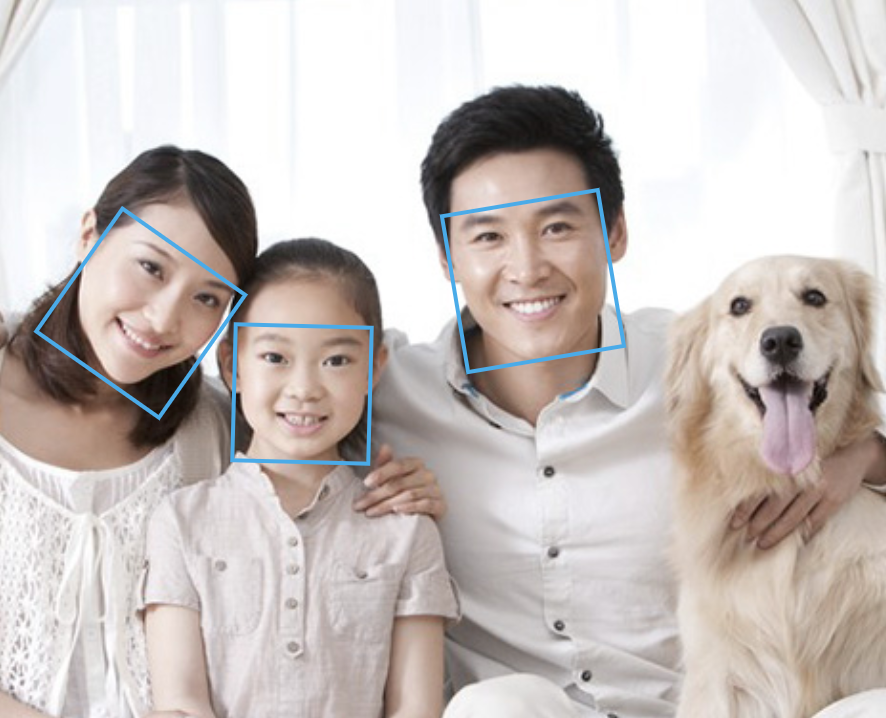
\includegraphics[width=8cm]{images/face_detcetion.png}
    \caption{人脸检测 \protect\footnotemark}
    \label{fig:face_plus }
\end{figure}
\footnotetext{https://www.faceplusplus.com.cn/}

人脸检测可能会遇到人脸过多、奇怪表情、面部朝向姿态、光照、分辨率、肤色等问题,特别是在非标准环境下,从复杂的图象中精确定位到人脸是非常有挑战的事情。

总的来说,人脸检测可以分为基于特征和基于图像两类,下文将分别介绍。

\subsubsection{基于特征的人脸检测方法}
基于特征的方法通过提取图像的特征,然后将特征与人脸特征信息进行匹配,这类方法主要代表有基于颜色模型的人脸检测\cite{dhivakar2015face}、ASM&PDM\cite{kumar2019face}、基于Gabor滤波器的人脸检测\cite{sharif2011face}等。

基于颜色模型的人脸检测通过将人脸图像映射到三位颜色空间进行简单判断。人的肤色是人脸中的一个非常重要的特征,使用人脸的肤色作为特征处理虽然准确率不高,但是速度快,计算简单。
当前主要使用的颜色模型有RGB、HSV、YCbCr等,以HSV颜色模型为例,HSV颜色模型中颜色由色相(H)、饱和度(S)、强度值(V)三个维度组成。
通过HSV颜色模型,使用简单的规则就可以过滤出肤色需要满足的条件:
$$
\left\{ 
\begin{array}{c}
    0 <= H <= 0.25 \\ 
    0.15 <= S <= 0.9
\end{array}
\right. 
$$

基于Gabor滤波器的人脸检测则通过将人脸图像映射到特征图像进行对比。在图像处理中,Gabor滤波器常用于作为算子获取图像的边缘和纹理特征\cite{sahib2020hybrid}。
由于人脸有着独特的轮廓特征,因此Sharif等 \cite{sharif2011face}提出了一个使用Gabor滤波器进行人脸检测的方法,
该方法使用40个Gabor滤波器为每个输入提供了40个特征图片,然后根据每个特征图片中强度最大的点与人脸库中对应的点进行距离比较,从而判断是否检测到人脸。

由上面两个例子可以看出,基于特征的人脸检测方法思想是尝试将人脸映射到另一个特征维度的以获取人脸的不变特征如眼睛、眉毛、嘴巴等,对特征脸的数据要求也比较小,实现起来简单。
但当人脸图像受到光线影响、被部分遮挡时,基于特征的方法准确率将大幅度下降。

\subsubsection{基于图像的方法人脸检测方法}
基于图像的方法人脸检测方法直接将输入图像与训练人脸图像进行匹配,这类方法主要代表有特征脸方法(EigenFace)、SVM、Haar分类器、基于人工神经网络\cite{farfade2015multi}的方法等。
这类方法不事先定义人脸的特征,而是采用训练数据的方式从数据中学习人脸的特征分布,在提供足够训练数据的情况下准确率相对基于特征的方法有了很大的提高。

Labeled Faces in the Wild (LFW)是著名的人脸识别测试集,一共有6000组人脸图像,其中包含一半的正样本和一半的负样本。
其中传统基于特征的检测方法,在LFW数据集准确率大概是60\%, 基于深度学习的检测方法普遍可以达到99\%以上的准确率,超过了人眼判断的97\%的准确率\cite{sun2015deeply}。

总的来说,目前人脸检测算法的准确率非常高,完全可以满足在面诊系统的预处理获取面部区域的需要。

\subsection{面部兴趣区域提取}
兴趣区域提取在面诊技术中主要指的是从人脸图象中切分并提取出面部(去除五官)、舌部、唇部等不规则形状区域的技术,
常见的方法有基于混合高斯模型(GMM)\cite{Hu2016Robust}、SegNet\cite{Badrinarayanan2017SegNet}、TCMINet\cite{li2020tcminet}等。
\begin{figure}[h]
    \centering
    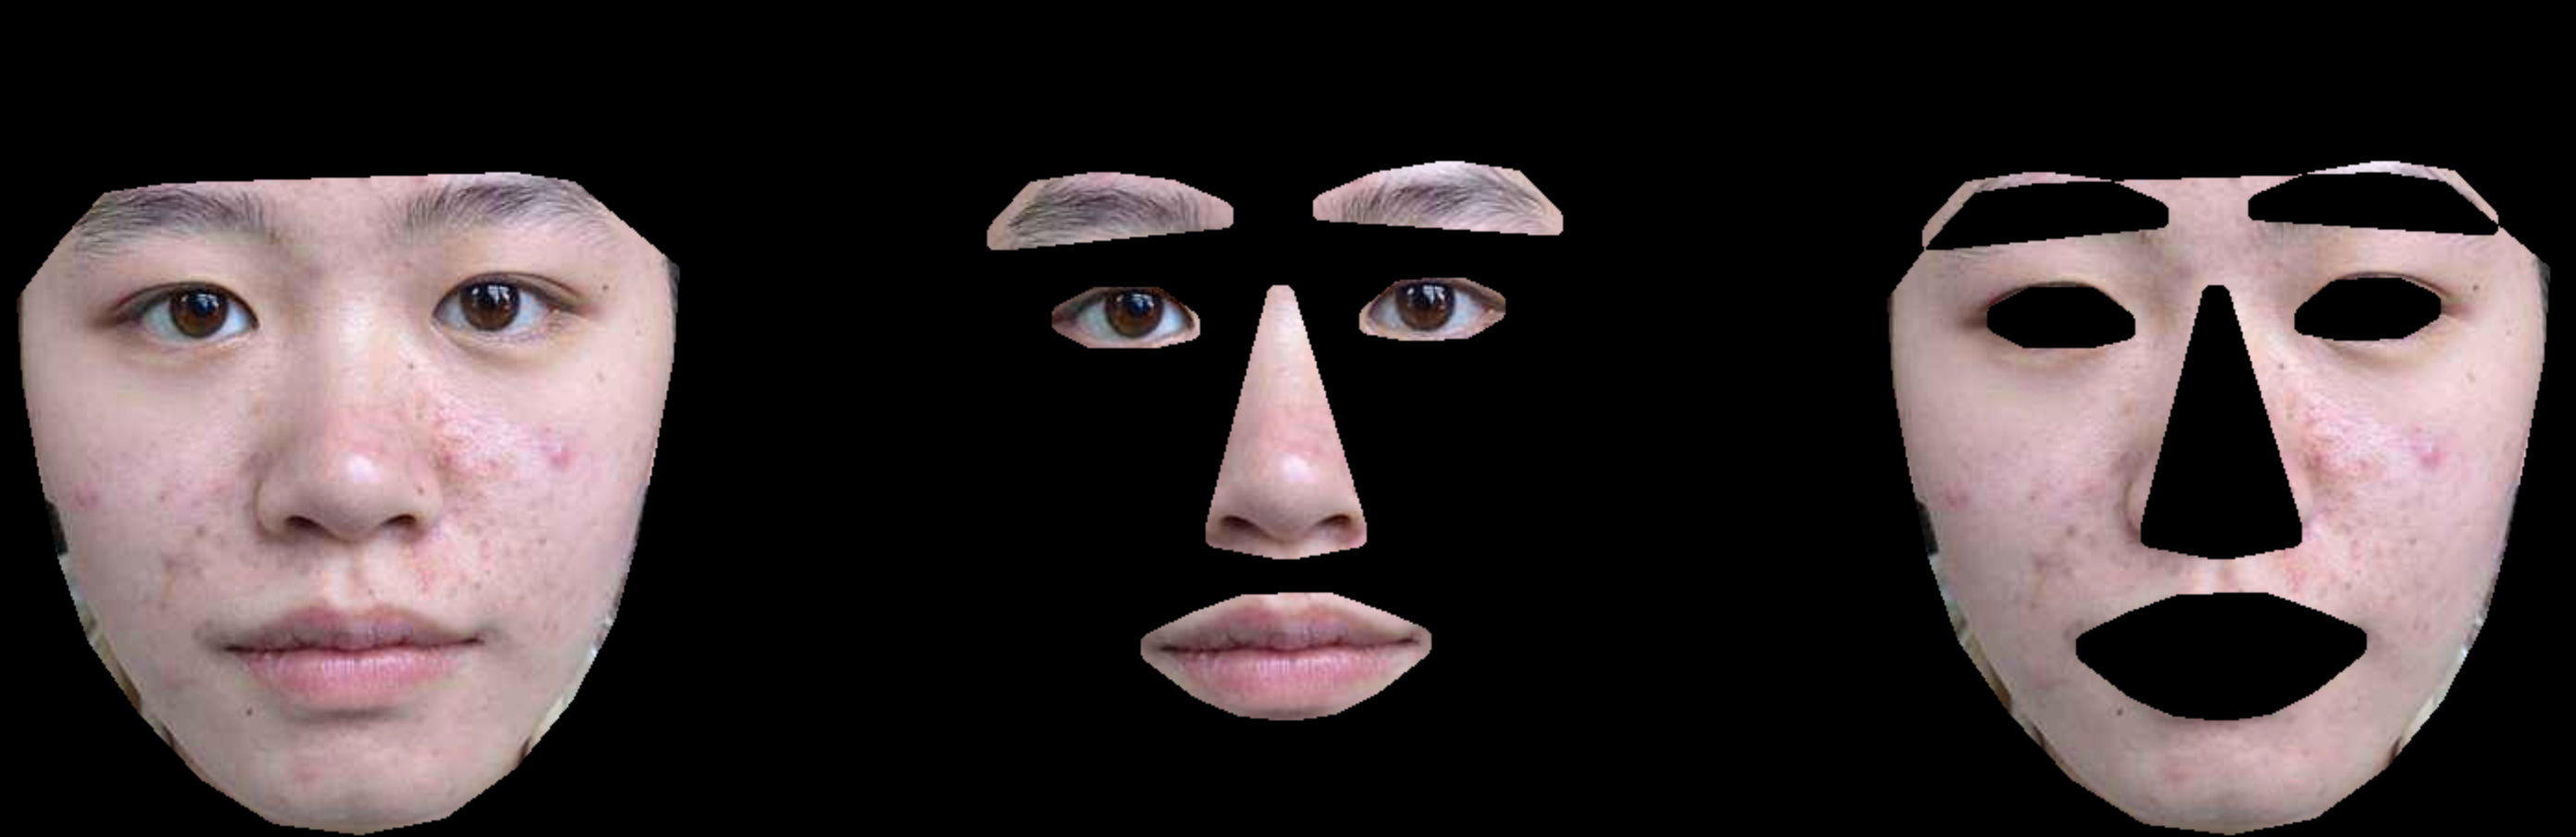
\includegraphics[width=12cm]{images/roi.png}
    \caption{兴趣区域提取}
    \label{fig:roi}
\end{figure}
本文在后续的系统实现中,主要使用了基于GMM方法进行兴趣区域提取,因此本小节将对其做简单介绍。

% 介绍单高斯模型

\subsubsection{混合高斯模型}
高斯分布也成为正太分布,是自然界大量存在的最为常见的分布模式。

\begin{equation}
    \mathcal{N}(x | \mu, \Sigma) = \frac{1}{(2\pi)^{D/2}}\frac{1}{|\Sigma|^{1/2}}exp\{-\frac{1}{2}(x-\mu)^T\Sigma^{-1}(x-\mu)\}
\end{equation}
% \begin{figure}
% \includegraphics[width=200pt]{Guassian.png}
% \end{figure}

混合高斯模型是对高斯的模型的拓展,假设数据的分布为多个高斯分布的叠加组成,相比简单高斯分布对复杂数据的刻画能力更强。
\begin{equation}
p(x) = \Sigma^K_{k=1}\pi_k\mathcal{N}(x|\mu_k,\Sigma_k)
\end{equation}
其中
\begin{equation}
\Sigma^K_{k=1}\pi_k = 1
\end{equation}

混合高斯模型在图像处理中经常用来完成图像分割任务:通过对图像中的像素点进行混合高斯模型建模,可以得到图像上每个点属于高斯模型的概率,进而通过概率值将图像分割为多个区域。

\subsubsection{兴趣区域提取过程}

利用混合高斯模型进行兴趣区域提取,可以截取唇部和舌部区域,以截取唇部区域为例,主要步骤如下:

\begin{enumerate}
    \item 使用人脸检测算法检测图片中是否包含人脸,裁剪人脸区域作为下一步输入。
    \item 对人脸上半部分无唇部的区域使用混合高斯模型获取当前图像的肤色概率分布p。
    \item 根据经验值,预先设置好肤色裁剪比例参数列表 it[N]。
    \item 迭代式地判断N次,对于每次迭代i,在人脸下半部分定位唇部:
        \begin{enumerate}
            \item 按照预先设置的参数it[i],通过比较每个像素点的肤色概率p[x]和参数t[i], 如果p[x]>t[i], 去除皮肤区域。最终得到去除部分肤色区域的图像。
            \item 在图像中根据唇部的形状与色彩特征,定位到唇部个数:如果个数为1标记为找到唇部区域,继续迭代;否则标记为未找到唇部区域,直接退出。
        \end{enumerate}
    \item 在上一步获取到的有唇部区域的图像中,按照图像中的肤色区域大小变化率绘制曲线,取曲线的局部最小值对应的唇部区域作为最终的唇部裁剪区域。
    \item 对唇部轮廓进行简化平滑处理,截取出唇部区域。
\end{enumerate}

在上述方法中,N为迭代次数,一般设置为14,裁剪比例参数为 \{0.6, 0.5, 0.4, 0.3, 0.2, 0.1, 0.05, 0.01, 0.005, 0.001, 0.0005, 0.0001, 0.00005, 0.00001\}。
该方法相比\cite{rahman2014lip, li2010automatic, li2020tcminet} 等方法相对简单且准确率相对比较高,鲁棒性更强。

% 与面部图像预处理不同,特征提取算法主要关于点在于如何从图像数据中获取量化的基础特征,如面色、唇色、舌苔类型等。

\subsection{诊断模型}

\subsubsection{基于规则的诊断模型}
诊断规则即通过专业的医学知识编写的一系列规则,是通过分析大量的临床医疗数据以及现有的结论,将诊断特征与诊断结果的关系进行量化\cite{牛欣2011中医四诊合参辅助诊断关键技术的数字化、量化研究},如:

\begin{lstlisting}[language={Python}, title=诊断规则]
    if (特征1>阈值1) then 结果=结果3
    if (特征2>特征3) then 特征3无效
\end{lstlisting}

由人工编写的一些固定规则,结合了人工的经验,能提供基本的诊断能力,但由于严重依赖规则、表达能力有限,目前主要用于减少其他模型的训练成本以及修正最终的结果。
目前各类诊所环境中使用的面诊仪,其主要用到的技术是通过上述的人脸检测、预处理和简单分类模型抽取特定特征,如面色、舌苔形状等,
然后系统通过一定规则提示医护人员相关信息,帮助医护人员判断健康情况。
如基于上文提到的颜色模型结合简单的规则,就能完成对慢性肾炎\cite{刘金涛2014基于数字化慢性肾炎湿热证面诊特征研究}、
冠心病\cite{陈聪2019冠心病痰瘀互结证面诊图像特征参数分析}等基本判断。

\subsubsection{基于算法的诊断模型}
随着面诊算法研究的进一步深入,机器学习以及深度学习快速发展,将面诊问题按照期望输出可以简化为分类、回归问题,
从而利用模式识别及深度学习中的方法解决面诊问题。
将面诊问题抽象为回归问题,可使用回归模型判断用户的健康指数以及患有某类疾病风险的概率;
将面诊问题抽象为分类问题,可使用分类模型抽取相关特征以及判断用户的体质类型、五脏特征等,以下简单介绍部分相关技术。

SVM\cite{cortes1995support}是统计学习方法中常用的分类模型,应用非常广泛。
SVM利用核函数将原始数据映射到高维空间,通过EM算法求解一个超平面,完成对原始数据的分类,能够在小样本、非线性的情况下保持优秀的泛化能力。
陈淑华等\cite{陈淑华2016面部颜色空间分析及其在疾病诊断中的应用}使用SVM分类器用于判断用户是否患有糖尿病、乳腺癌、胃炎等五种疾病,
在其数据集上判断健康与非健康能达到70\%的准确率,五种疾病平均准确率能达到79\%左右;

卷积神经网络\cite{li2016survey}是指基于卷积、激活、池化等基本结构组成的神经网络结构,经常用于处理各种图像、文本、音频相关的任务中,具有非常强的泛化能力,
将其用于面诊问题能达到更高的准确率。
Liang\cite{liang2020oralcam} 在移动设备上实现了OralCam系统:
该系统使用深度卷积神经网络判断用户口腔图片是否有口腔疾病的五个特征,从而帮助用户提高口腔健康意识。
端到端(即直接将面部图片进行输入,不做手动特征提取)的模型设计往往需要大量的样本数据支持,而迁移学习能降低模型对数据量的要求。
Jin \cite{jin2020deep}等根据地中海贫血、甲亢病人脸部数据集,将在人脸识别数据集上预训练的卷积分类模型,迁移到面诊场景用于通过面部图片判断地中海贫血、甲亢病等,
其准确率达到90\%, 优于专业医生进行面诊得到的结果;

在本文的研究中主要关注交互与系统如何设计,诊断模型只作为研究系统特点用到的工具,对模型的准确率无过高要求。
考虑到SVM模型在解决特定诊断问题也有不错的效果,使用也相对比较简单,最后本文采用了SVM模型结合诊断规则的方式实现面诊系统。

\section{系统设计相关技术}
微服务是当前发展迅速的服务架构\cite{jamshidi2018microservices},能有效减少系统耦合性,提高系统拓展性等。
根据面诊服务实际需要本文并没有照搬整套微服务设计而是针对性地做了实现,本小节介绍本文在系统设计上用到的方法和相关技术。

\subsection{读写分离设计}
随着系统的吞吐量增加,数据库的读写往往会成为系统的瓶颈。
读写分离将数据库拆分为读库和写库,读库只负责数据的查询操作,写库处理事务性的增删改操作。
读写分离的主要目的是避免数据在更新过程中收到数据的查询请求而导致的行锁,
以提高系统吞吐量。

在数据库层面实现读写分离能提高系统吞吐量,但由于存在主库到从库的数据同步,会导致数据时效性延迟,且增加从库有额外的计算和存储成本。
不依赖数据库的读写分离设计,系统在设计层面也应该尽可能遵循读写分离的设计,如在模块或者方法层面尽可能避免同时读写数据库同一行记录;
对系统进行拆分,将写和读拆分为两个系统,两个系统之前通过消息的方式进行通信,通过缓存提高读服务性能等。

\subsection{主从模式设计}
主从模式设计在处理可分解问题时非常常见,其主要设计思想是为了解决单计算实例处理问题性能有限的问题,
同时也用于实现服务的高可用,目前在多个知名项目中使用,如Redis\footnote{https://Redis.io/}, ElasticSearch\footnote{https://www.elastic.co/}等。
主从模式将系统设计成多个节点,一般分为一到两个主节点和多个从节点,通过主节点将任务进行拆分,拆分成多个可分开执行的子任务,
然后将子任务分配到从节点中运行,运行结束后再将结果汇总返回。

主从模式的优点在于任务的并行处理,提高整体性能,此外多节点的方式具有容错机制,提高系统稳定性。
在实现上,主从模式关注以下两个方面:
\begin{itemize}
    \item 容错管理机制。当从节点崩溃或者上线时,其他节点需要感知,目前主要通过心跳包的方式实现节点鉴活,提供服务发现机制或利用现有的服务注册框架如Consul\footnote{https://www.consul.io/}、 Nacos\footnote{https://nacos.io/}等;
    当主节点崩溃时,其他节点可以完成主节点的选举和更换,目前有大量一致性算法如raft、paxos等。
    \item 服务间通讯方式。多个节点之前如何高效地完成同步、异步的通讯,目前实现方式有http/rpc调用,提供回调接口,消息队列,中心存储等。
\end{itemize}

\subsection{容器化技术}
容器化技术是Linux系统基于Namesapce和Cgroup等机制提供的内核轻量级的虚拟化技术,实现了服务间的资源隔离,方便快速构建部署服务。

\begin{figure}
    \centering
    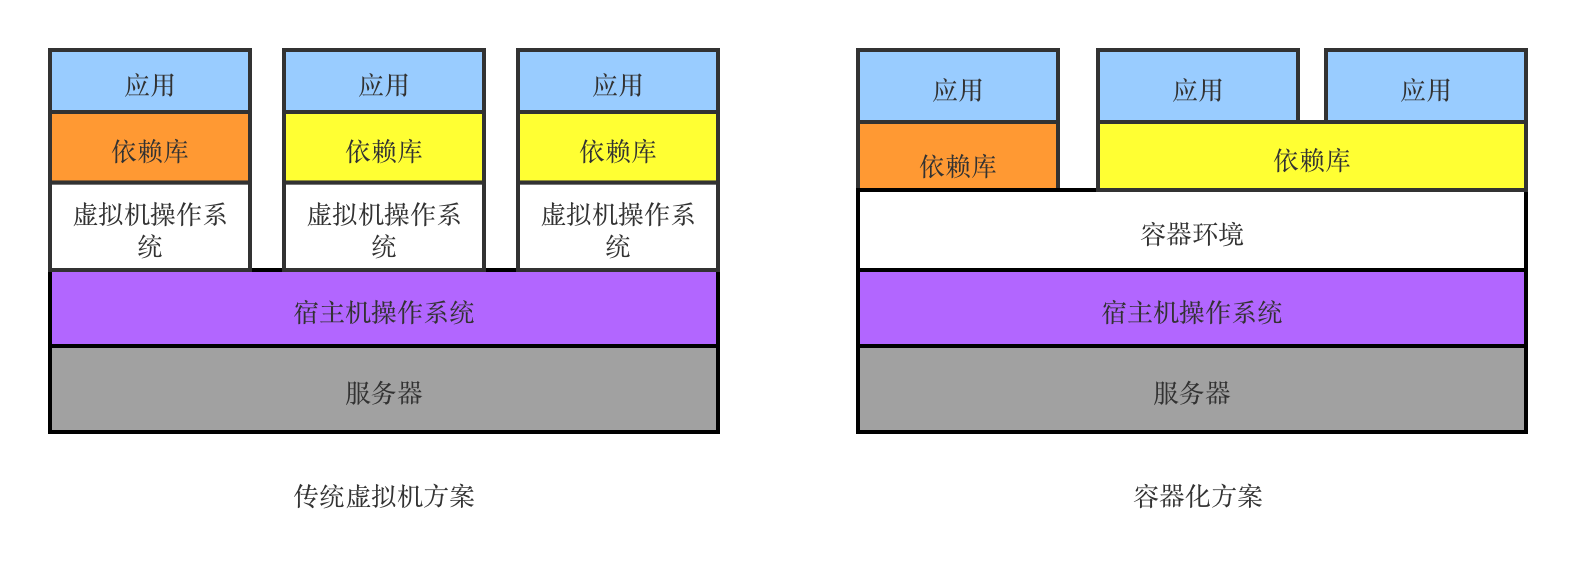
\includegraphics[width=12cm]{images/container.png}
    \caption{容器化vs虚拟机}
    \label{fig:container}
\end{figure}

和传统的虚拟机方式相比,容器化技术启动更快,资源占用更少,性能更好,目前主要的容器化解决方案有Docker及K8s。

Docker\footnote{https://www.docker.com/}是当前最流行的容器化解决方案,其有几个重要概念:镜像、容器、仓库。镜像提供了容器运行时需要的依赖、相关文件和环境变量等;容器与镜像的关系相当于进程与程序文件的关系:镜像成功启动后,就是一个容器;仓库为各类镜像提供了统一的管理平台。
基于以上设计,Docker提供了容器运行、镜像构建、镜像管理等基本功能,方便用户将快速部署代码,将系统服务化。

K8s(kubernetes)\footnote{https://kubernetes.io/}是基于Docker(但不局限于)的容器编排工具,提供对容器集群的部署、拓展、管理等功能,
基于K8s可以快速搭建出一个集群服务。

模型服务化是指将算法和模型等打包成可调用的服务,
目前主流的做法就是利用Docker将模型需要的依赖和环境打包到Docker镜像中,以HTTP Server或者RPC的方式对外提供调用接口。

\section{本章小结}
在本章中,首先介绍了下一章将要用到的技术探针方法,然后介绍了相关人脸检测算法、本文用到的面部兴趣区域提取算法、诊断模型等,
最后介绍了本文在系统设计中用到的容器化技术和相关系统设计方法。
% 3.前期用户调研
\chapter{用户调研}

% 介绍为什么要做这个
为了研究日常使用场景下面诊技术的应用会遇到的问题,本文首先利用技术探针\cite{Hutchinson2003Technology}的方法进行了定性研究,通过分析访谈数据来探索和总结面诊应用在日常场景下的特点和存在的挑战。


\section{技术探针}

% 为什么要用技术探针
在日常场景下,典型的HCI交互设计方法是访问用户的家庭,然后设计并实现一个系统,再测试用户喜欢或者不喜欢。在日常场景下,这种设计方法缺点比较明显:

(1) 没有激发用户的思考,可能无法反映用户的实际需求和掩盖在家庭内部之间“好玩”的设计;

(2) 在设计和实现系统过程中,没有提供真实的长期使用场景,用户缺乏参与性。

% 介绍什么是技术探针
为了避免上述的问题,Hutchinson等\cite{Hutchinson2003Technology}提出了一种利用快速开发出来的、功能并不完善的原型系统,让用户在实际使用原型系统的过程中,鼓励用户大声表达自己异想天开的想法,在草稿上画出自己心中的系统,参与设计过程的研究方法。

基于技术探针的方法经常被用来为日常使用的健康技术的设计提供信息。例如基于技术探针的设计方法,Papi等人\cite{papi2015knee}利用可穿戴式膝关节原型,探索了在家庭环境下如何设计用于骨关节炎患者的康复工具;同样,Singh \cite{singh2017supporting} 等人通过1-2周的用户调研,利用技术探针,研究了如何设计慢性疼痛患者使用的日常可穿戴设备。

\begin{figure}[h]
    \centering
    \subfigure[主界面]{
        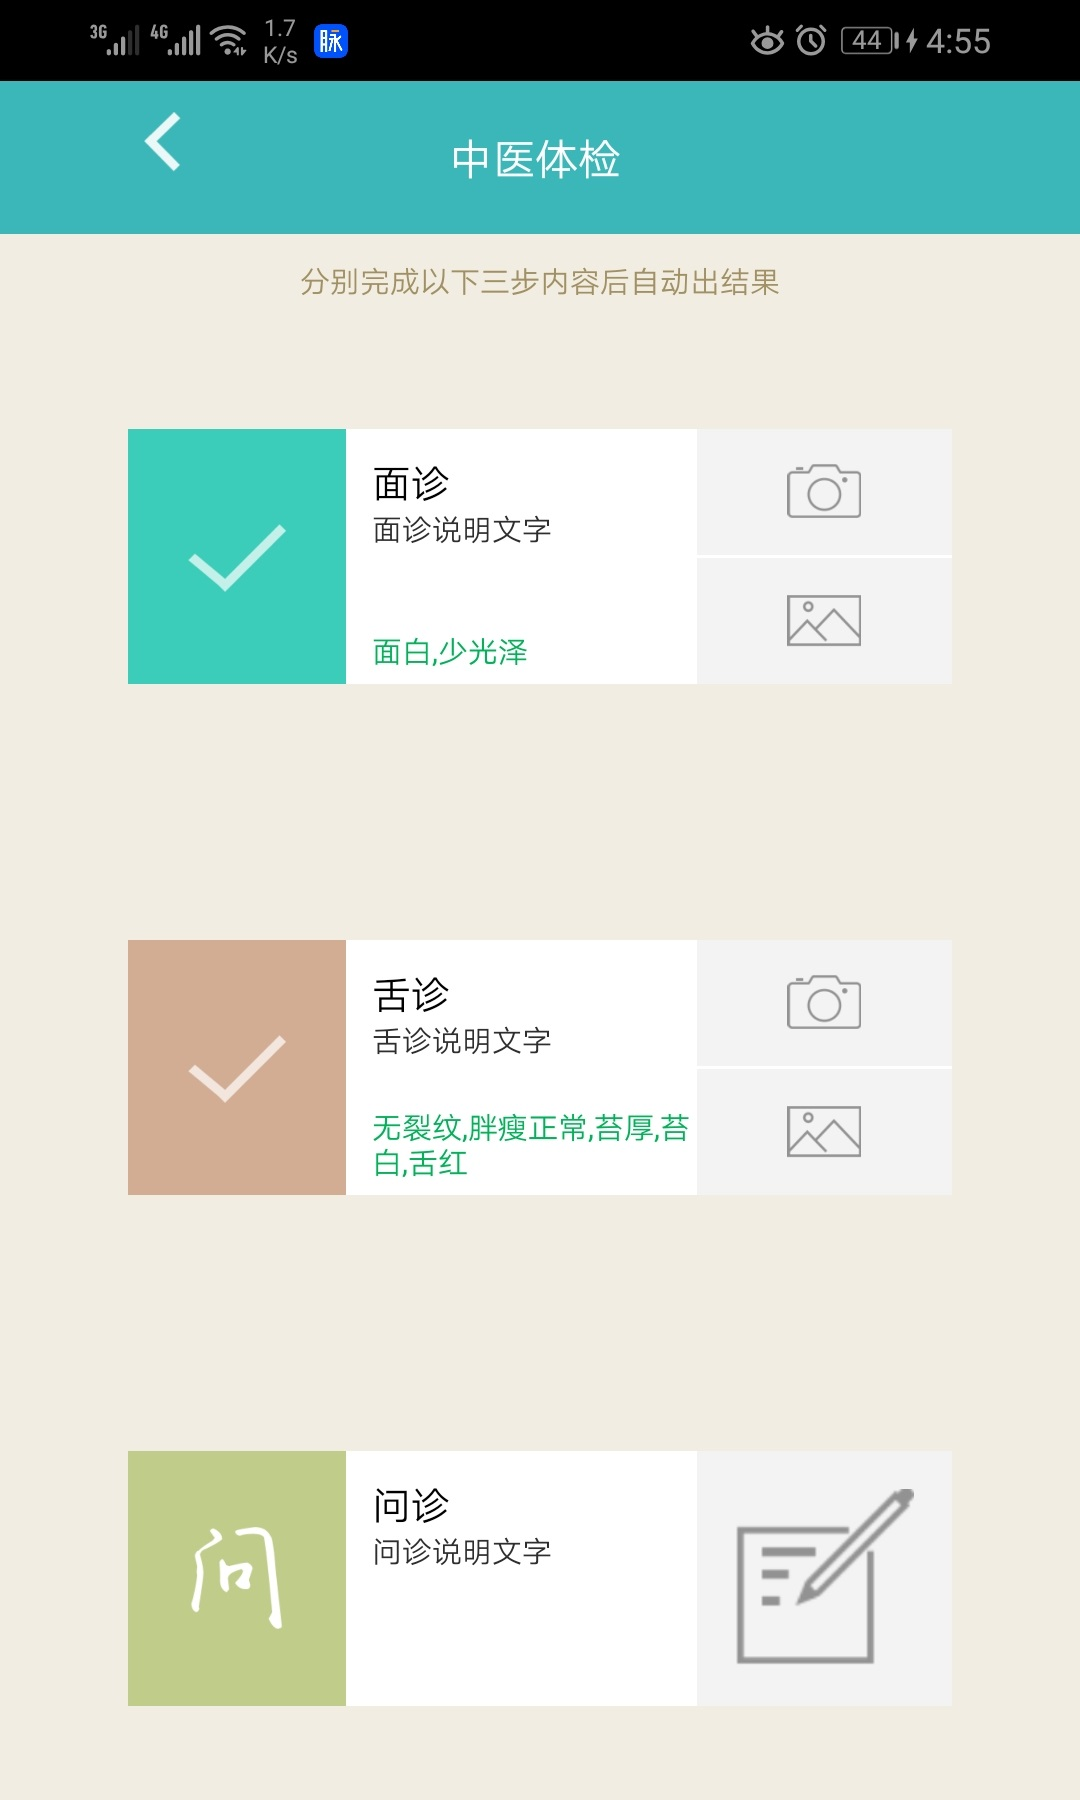
\includegraphics[width=4.5cm]{images/main1.jpg}
    }
    \subfigure[问诊]{
        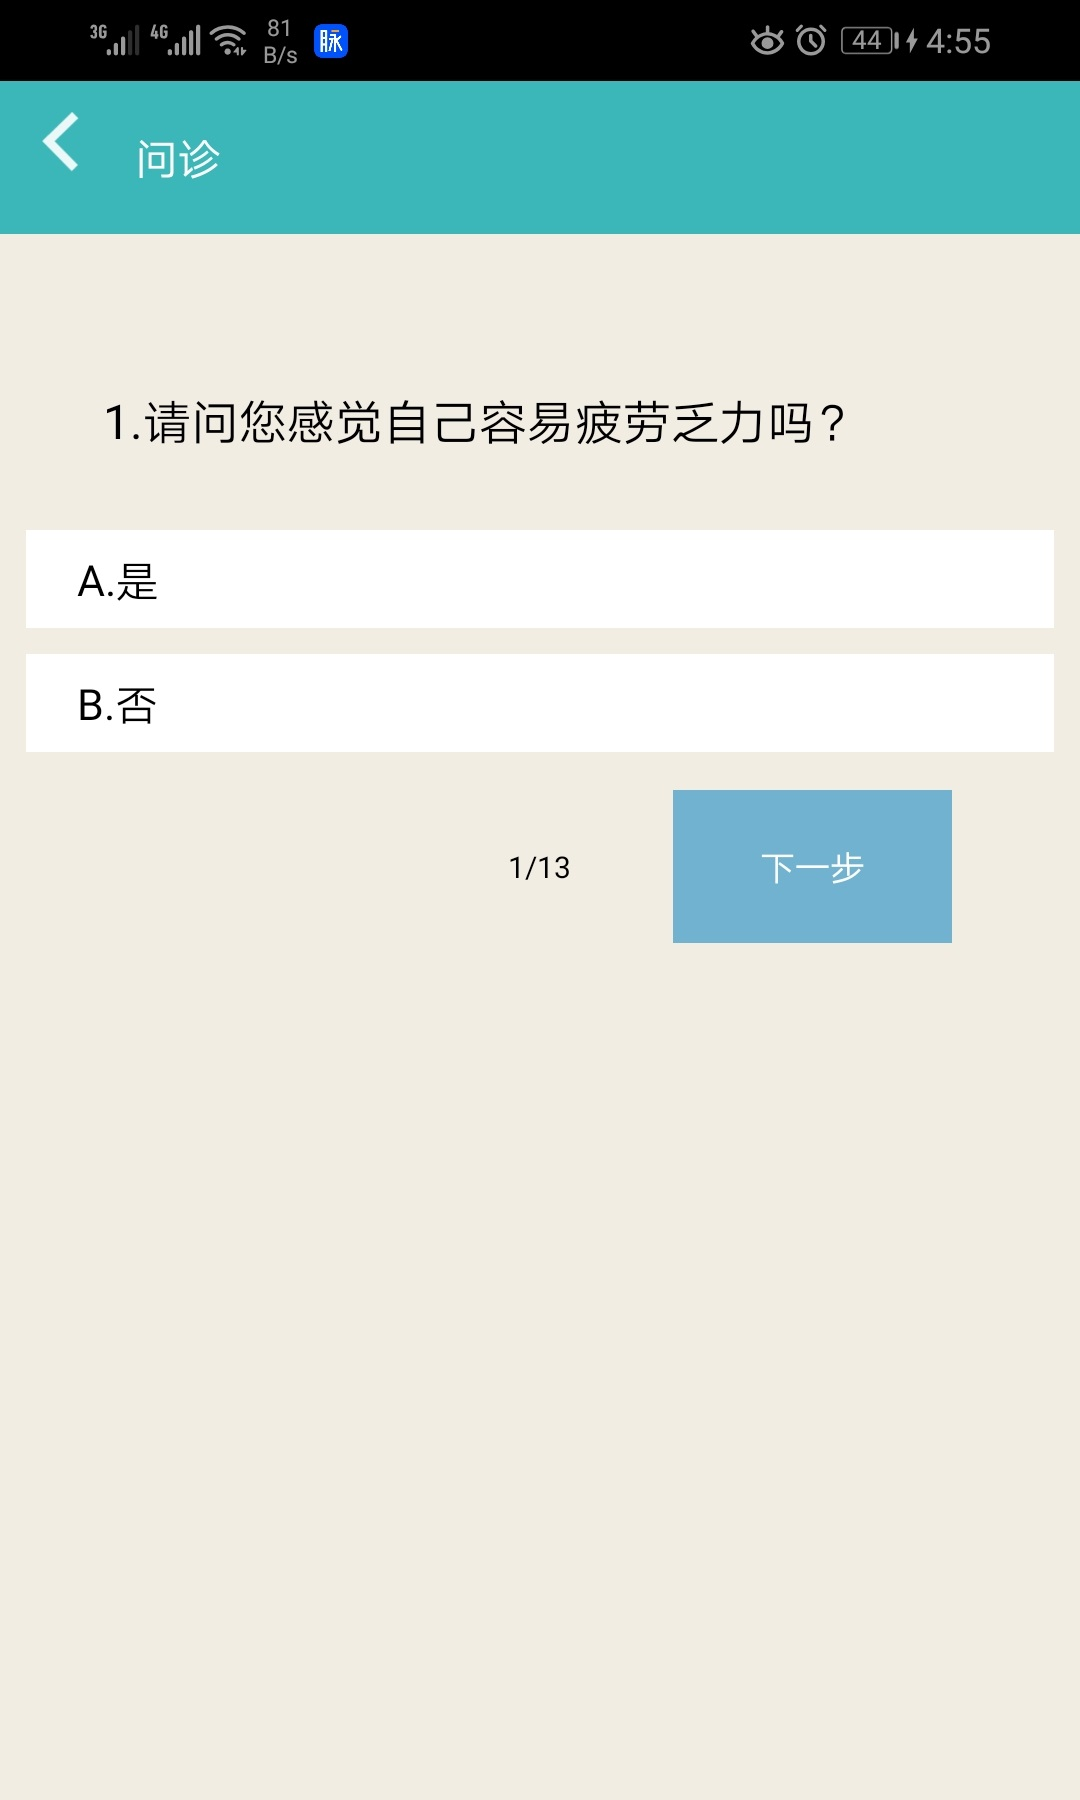
\includegraphics[width=4.5cm]{images/main2.jpg}
    }
    \subfigure[健康报告]{
        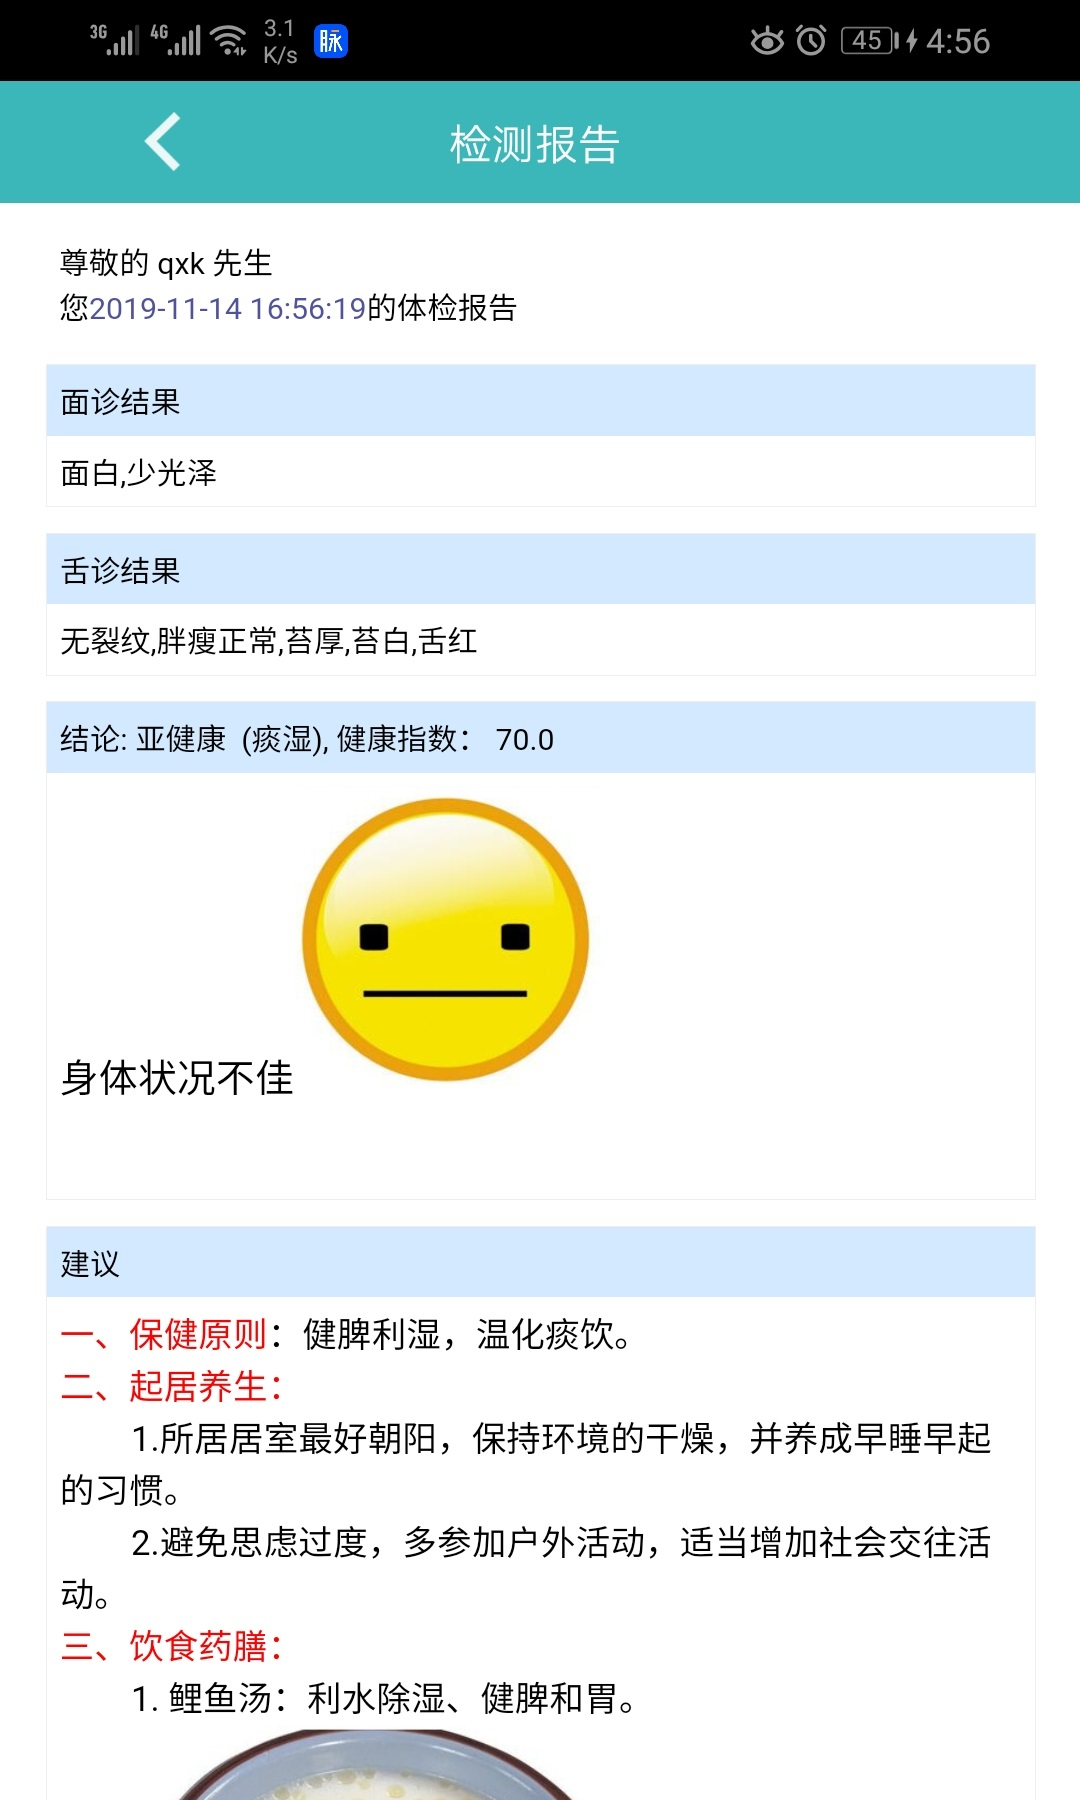
\includegraphics[width=4.5cm]{images/main3.jpg}
    }
    \caption{技术探针}
    \label{fig:main}
\end{figure}

为了方便进行快速用户调研,我们选用了云中医\cite{Zhang2018Study}作为技术探针。
云中医是复旦大学计算机学院张文强老师和上海中医药大学合作开发的一款面诊应用,虽然它的主要应用场景是诊所内,且由于准确率的原因,结果只能做参考,但是它实现了面诊,舌诊和问诊的基本功能,符合技术探针的要求。

云中医是一个手机上的健康诊断应用程序,旨在提供一个方便的平台的自我诊断和健康管理。该应用以中医面诊、舌诊、问诊理论为指导,在手机上模拟实现了诊断的过程:
用户需要依次对自己的面部和舌头进行拍照,回答一些与自己健康状况相关的问题,最终会收到一份完整的健康报告和一些健康建议。

云中医app的主要界面及使用流程如图 \ref{fig:main}所示:用户进入诊断页面之后,会看到三个区域:面诊、舌诊、问诊。面诊和舌诊通过拍照或者上传图片完成,问诊是通过依次回答13个问题来完成。
依次完成面诊、舌诊、问诊之后,系统会给出用户的体质和健康分数,并且给出对应的健康建议。

\section{定性实验}
 
% 介绍定性研究
本实验采用的是定性研究方法。定性研究是广泛应用在用户需求调研、人机交互、心理学等领域的研究方法 \cite{崔岩2011统计分析中的定量与定性研究}, 常见的收集数据的方法包括深度访谈、焦点小组访谈、日记、观察法等 \cite{李晓凤2006质性研究方法}。

% 研究方法 -> 研究过程->数据采集->数据分析->得出结论
为了尽可能详细地理解用户在日常健康场景下使用面诊技术的各种行为和态度,我们采用半结构化的深度访谈来收集定性数据\cite{DiciccoThe}。深度访谈是定性研究领域中收集数据最常用的一种方式,通过开放式、半结构化的面对面访谈,能够深度了解调查者内心的客观想法,避免研究者的主观判断。

\subsection{实验过程}
\begin{figure}[h]
    \centering
    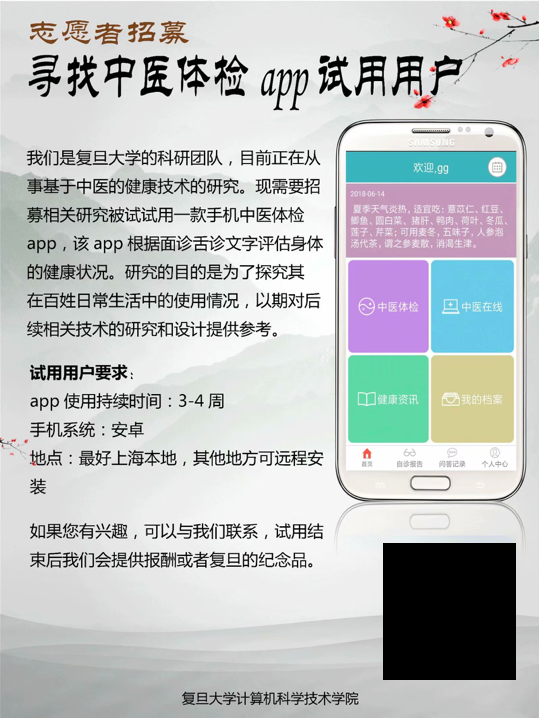
\includegraphics[height=15cm]{images/poster.png}
    \caption{招募海报}
    \label{fig:poster}
\end{figure}

% 人员招募

\begin{table}
    \centering
    \begin{tabular}{llll}
          \toprule
          编号 &	性别 &	年龄 &	职业 \\
          \midrule
          参与者1 &	男 &	20多 &	博士生 \\
          参与者2 &	男 &	20多 &	研究生 \\
          参与者3 &	男 &	20多 &	研究生 \\
          参与者4 &	女 &	50多 &	医院护理工 \\
          参与者5 &	男 &	40多 &	办公室职员 \\
          参与者6 &	女 &	40多 &	小学老师 \\
          参与者7 &	女 &	50多 &	办公室职员 \\
          参与者8 &	女 &	19岁 &	本科生 \\
          参与者9 &	男 &	20多 &	办公室职员 \\
          参与者10 &	女 &	40多 &	办公室职员 \\
          \bottomrule
    \end{tabular}
    \label{tab:Participants}
    \caption{参与者}
  \end{table}
  % 实验过程
  我们通过社交媒体发布海报(如图 \ref{fig:poster}所示)招募志愿者参与实验。通过宣传,我们最终招募到了10位感兴趣的志愿者,志愿者资料如 \ref{fig:Participants} 所示。在招募到合适的用户之后,我们会对每一个用户进行一次采访,主要是为了了解用户信息,介绍技术探针。采访是在征得志愿者的同意下,全程录音的情况下进行的。

% 在被试人员对此应用感兴趣,愿意尝试的前提下,尽量使得招募到的人员在年龄、健康状况、教育背景、工作性质等方面具有多样性。不同的年龄层次可能会导向对健康的不同关注角度(中老年人较为关注的养生知识逐渐在青年群体中流行起来)不同的工作性质使得人们重点关注的身体部位不同(白领普遍关注的肩颈,特殊行业的“职业病”)不同的教育背景使得人们对用技术手段监测健康信息的接受程度也有差异。

接下来两周时间,让用户在日常场景下使用应用。在第一星期,我们不做任何干预;到了第二星期,要求用户每天至少使用一次。

在用户使用结束后,我们会进行一次结束后的回访,了解用户在使用中遇到的问题和他们的想法。

我们希望通过此次调研了解到使用面诊应用的用户群体有哪些?用户期望通过面诊应用来获取哪方面的信息?以及在方便用户日常使用上,有哪些待解决的技术难点?为了回答这些问题,我们通过分析采访数据进行探索。

\subsection{数据分析过程}

\begin{table}[h]
    \begin{tabular}{ll}
        \toprule
        编号 & 问题 \\
        \midrule
        1  & 您的年龄?职业背景?   \\
        2  & 您目前健康状况如何?平时感觉身体哪里不舒服吗(慢性病,容易疲劳,关节疼痛等等)?   \\
        3  &  您有使用健康状况评估的技术吗?若有,都有哪些技术?平时如何使用的?使用体验如何?  \\
        4  & 有看多中医吗?是什么原因看的中医?在哪里看的?效果如何?   \\
        5   & 对中医的面诊、舌诊有了解吗?若有,通过什么渠道了解的?   \\
        6  & 平时会留意自己的面色,舌苔吗?会留意其他人的面色,舌苔吗?\\
        7   & 您对这个APP感兴趣的点主要在哪里?\\
        \bottomrule
    \end{tabular}
    \caption{第一次采访问题大纲}
    \label{tab:inteview_questions}
\end{table}

介绍性的问题大纲如 \ref{tab:inteview_questions}所示,我们会根据访谈的深入不断迭代问题大纲。
我们将每个用户对应的采访和回访的录音转录成文字,最后整理后一共有56页的采访数据。由于采访数据量比较大,本文采用主题分析法(Thematic Analysis)进行数据分析工作,大致分为以下几个步骤\cite{SchwandtQualitative}:

(1) 数据精简(data reduction)。对访谈记录中的数据进行删减,只提取关心的内容。

(2) 数据展示(data display)。对保留的内容进行分类,从中提取关键词。然后再根据关键词提取出新的分类,由新分类返回到第一步循环提取相关的内容。反复迭代步骤(1)和步骤(2), 知道无法提取出新的内容和新的关键词为止。

(3) 归纳主题(conclusion drawing)。主题是对关键词所反映的内容模型的抽象化,在访谈数据中不断重复出现并且具有共通性,通过主题能够将提取出来的关键词联系起来对访谈的内容进行解释。

\section{研究发现}

通过对采访数据进行分析,我们的用户调研发现如下:
\subsection{潜在的使用场景}
通过调研,我们发现面诊类应用在日常使用环境下,用户反馈有两种潜在的使用场景:

\subsubsection{1.了解身体状态}

对于那些已经有健康问题的用户或者日常有养生活动的用户对云中医更加感兴趣,并且知道如何在日常生活中使用它。

参与者1他从小就是一个病骨头,总是生病,所以经常看中医。参与者1说道:\myfont{像我这种生了病或者健康状态不好的人,是可以用云中医应用来日常使用来检测疾病的。}
参与者10对云中医应用也表现出浓厚的兴趣:\myfont{这些诊断结果和建议对我很有用,因为在手机上做诊断很方便,我一有空就会用一用。比如我今天早上有空,我就打开用了一下。}
参与者3是一个对自己健康状态很看重的人,他说道:\myfont{因为它可以进行面诊和舌诊告诉我结果,并且给出了一定穴位按摩的建议,我觉得很有用。}

大多数参与者使用云中医不只是为了了解自己身体的状况,更是为了能够及时调整自己的生活方式。
如参与者3有一次早上感觉非常疲倦,于是他拿出云中医应用对自己进行了诊断,果不其然应用给出的分数是自使用以来最低的65分,他觉得这类应用非常重要:\myfont{作为一名学生,久坐是不可避免的。当我感觉疲倦的时候,我就打开云中医看一下,然后根据结果来决定是不是要去锻炼一下。}
参与者1也提到云中医可以帮助进行健康决策:\myfont{云中医可以帮我了解自己的身体状况,这样我就可以判断自己当天是否可以加班了。}


\subsubsection{2.医患沟通的工具}

正如其他健康跟踪类技术的发现类似,参与者希望云中医能够提供医生和患者沟通的渠道,这样医生可以更好地获取病人的日常健康信息。

参与者8说道:\myfont{这类应用可以和医生合作,这样医生就可以获取患者的健康状况并及时发现问题}, 她进一步建议:\myfont{可以把每次的诊断结果保存到个人档案中,这样医生可以方便地获取到患者的健康信息,这样医生就可以知道患者在就医期间的日常健康状况了。}

\subsection{自适应性}
日常环境和诊所环境不同,日常环境下需要用户长期使用。但是,大部分的参与者在使用云中医一到两次后就不再使用了,其中一个重要的原因就是云中医缺乏自适应性的能力。

比如参与者1在采访中指出:\myfont{无论我什么时候拍照,它都是问我同样的问题,我会感觉很无聊。}
同样,参与者2说:\myfont{每次都重复地检查很枯燥。}参与者6解释了她不继续用云中医的原因:\myfont{一个人的健康状况,在短时间内的变化不会太大,所以我就没一直用了。}
而参与者7虽然在持续使用,但是也不愿意每次看到相同的信息:\myfont{它每次都给我相同的健康结果,我怀疑它的准确性。}

参与者在提出问题的同时,也给了对应提高系统自适应性的建议,主要体现在两个方面:

\subsubsection{1.自适应用户信息}

从调研反馈来看,我们发现因为云中医在问诊的时候,一直问用户同样的问题,而实际情况是短期内来说,大部分问题的答案是不会发生改变的,这样缺乏用户信息的自适应性会让用户使用起来觉得很繁琐。

在这次的用户调研过程中,在诊断应用的场景下,我们发现用户强烈希望系统能够记住他们的用户信息并对下一次诊断进行相应的调整。
比如一些参与者抱怨说每次去回答问诊的问题非常地繁琐, 参与者2说道:\myfont{问诊那一部分设计地不好,每次问题都是固定的,而且太笼统了。},然后他建议这些问题应该更加个性化:\myfont{我认为问诊的问题可以根据之前问的问题更加地具体。}
参与者10则希望系统能够追踪用户的健康状况:\myfont{我希望它有后续的追踪过程,不仅可以评估当天的健康状况,也可以在接下来的几天内,跟踪健康问题并动态地调整建议。}
参与者3也有类似的想法:\myfont{目前系统只有诊断的功能,我希望系统能够接受用户的反馈,比如记录系统给出的健康建议是否有效,这样可以调整健康建议的结果。}

\subsubsection{2.自适应环境信息}

系统给出的养生建议也是固定的,并没有考虑到用户当前的工作状态和环境因素。中医认为,于环境变化和谐相处对于保持健康很重要,特别是在季节变化的时候。

参与者6建议:\myfont{养生建议应该更加丰富一些,比如考虑季节和节气的变化。} 
参与者10希望系统能健康建议和当前天气综合考虑:\myfont{那么热的天气叫我出去运动? 它应该考虑到我个人的健康情况和当前的天气情况。}

\subsection{实用性}
在调研过程中,我们发现并不是所有的参与者都能接受健康报告的结果,主要原因有以下两个方面:

\subsubsection{1.中医术语}

云中医应用是和上海中医药大学一起合作研发出来的,健康报告的文字使用的是标准的中医术语。和平时就医环境不同的是,在日常环境下,用户在使用的时候,周围是没有专业的医生可以询问的,因此通俗易懂的解释中医术语是非常重要的。
在调研过程中我们就发现很多参与者很难理解系统给出的健康报告,特别是在年轻群体中,新一代年轻人对中医的接受程度比较低,这个问题就更加严重。
参与者2是在读研究生对健康报告的里“气”的概念就不是很了解,他提到:\myfont{我对中医知之甚少,它说我气虚,但是什么是气虚我都不知道……}
参与者8也觉得自己对中医知识了解有限,对结果不是很理解:\myfont{分数下面有提到五脏的概念,但是其实我连五脏指的是哪五个器官不是很清楚,可能包括肝脏、心脏和肾脏?}
虽然中医在中国的历史悠久,但是并不是所有的人都清楚中医中的常见概念。 如果系统是设计给普通用户日常使用的话,就需要考虑到用户的中医知识素养了。

解决此类问题的方法之一,是把中医术语和常见的词语进行关联。比如参与者1遇到这样一个例子:\myfont{我今天感冒了,但是系统却没有提示我感冒了,只是说我气血不畅,它为什么不直接告诉我感冒或者风寒呢?}

另一个解决方法则是通过更加生动的方式进行介绍,比如视频图片等。还是参与者1,他说:\myfont{健康建议里的按摩,可能直接给出一个按摩的视频,而不是只有文字和图片,有一个视频跟着做的话会更好。}

参与者还提出可以通过提供学习的机制,让用户了解晦涩的中医术语。
事实上在调研过程中,就有参与者把云中医当作一个学习中医养生的工具,例如参与者10提到:\myfont{我认为系统可以提供更加宽泛的养生知识,而不只是健康建议。我对健康建议中的穴位按摩就很感兴趣。}

\subsubsection{2.养生建议合理性}

不同职业的用户,日常的空余时间是不同的。空余时间是否充裕,是影响用户实践养生建议的关键。因此系统给出的养生建议,特别是需要花费较长时间的按摩熬粥之类大的养生活动,需要合理考虑用户的日常空余时间。

比如参与者2就指出:\myfont{作为一个住在没有厨房的公共宿舍的学生,养生建议中的食疗就是不切实际的。我不会做饭,而且有些食物用的材料太贵了,超出了我的承受范围。}
参与者9是一位刚参加工作的算法工程师,每天8点才下班,他反馈说:\myfont{我基本没有什么时间熬粥或者煎药了。} 参与者7表示:\myfont{每天都进行穴位按摩太费时间了,我坚持不下来。}

\subsection{敏感性}
\subsubsection{1.文化敏感性}

舌诊的时候,需要用户伸出舌头进行拍照,这个过程可能会给用于带来烦恼。
在中国文化中,伸出舌头可以表示厌恶或者无礼,并且大部分中国人是比较传统的。因此在很多情况下,在公众场合伸出自己的舌头被认为是不合适的。大部分参与者表示伸出舌头会让他们感到尴尬,或者是害怕自己因为伸出舌头在无意间冒犯到别人。
如参与者1认为,伸出舌头拍舌头的照片是很不雅的。参与者3表示自己在和别人拍照的时候都会感到紧张,使用云中医时都是私下使用。特别是年轻人来说,参与者8直白地指出伸出舌头这个动作太丑了,她只会在私人空间下使用应用,她甚至调侃说:\myfont{我觉得这个软件是太有意思了,因为它有拍舌头的各种照片,完全就是收集丑照的一大利器。}

不过有趣的是,对于年纪稍大的参与者或者老年人来说,对于伸出舌头进行诊断并不是非常在意。例如参与者10说:\myfont{我并不觉得尴尬,因为这是一种诊断。}, 参与者4对这一现象解释说: \myfont{对于像我这样的年纪的人来说,就不那么在乎了}。 

总而言之,这个发现提醒了我们文化敏感性限制了面诊类应用的日常使用范围。

\subsubsection{2.技术敏感性}

由于模型的计算需要对面部舌部图片进行颜色特征的提取,使其对外部因素如光照和手机摄像头的质量会更加敏感,已经严重影响了部分用户的使用。
参与者7在系统一次又一次提示检测不到照片中的人脸之后选择了放弃:\myfont{照片一直提示重拍,觉得麻烦就不用了。}
参与者8还特别反映了自己用的是vivo手机,拍照会受到相机自带美颜算法的影响: \myfont{但是你需要考虑,我现在用的手机是vivo手机,它的相机自带美颜的功能。你把照片传过去,那准确率不就下降了吗?}

由于目前技术的问题,环境和设备的多样性不仅可能降低最终结果的准确率,甚至会影响用户的正常使用。因此,在离开诊所环境下严格统一的光线和设备条件之后,将面诊应用日常环境下,从技术的层面来讲,需要考虑更多的因素。
或者说,在技术无法改进的前提下,我们应该如何设计系统来屏蔽这些环境因素和设备的差异性,也是一个需要考虑的问题。

\subsubsection{3.社交敏感性}

虽然有几位参与者希望分享它们的健康结果给其他人作为相互学习的机会,但是他们同时也担心因为涉及到面部照片和个人健康信息,可能会导致隐私泄露的问题。
如参与者10讨论了可接受的分享的范围:\myfont{我觉得,比如说有什么症状我可以分享。比如说我今天有哪里不舒服了,得到了哪个专家的帮助,然后经过一段调理,我觉得我有好转了。但是有些可能关系到自己个人隐私的事情,我还是有点不愿意分享的。}

大部分参与者虽然不太愿意分享自己的诊断结果,但是如果将分享的范围限制在家庭或者医生圈子等可信任的人之内的话,他们表示可以接受。不过有趣的是,我们发现和其他社交分享类应用不同的是,对于家人来说,他们更加愿意分享给陌生人,因为分享给家人的话可能会引起家人不必要的担心,如参与者3表示: \myfont{其实我觉得分享的话更倾向的是和一些陌生人分享,如果和亲人分享的话,就觉得反而让他们,但是反而觉得是一种负担,如果和陌生人分享,就会觉得这是一个这一个交流的,就是一个也算是一个社交的一种方式吧,同时也能提高自己的健康知识。}


\subsection{信赖与情绪的问题}
关于用户对于日常面诊技术的态度,我们在本次用户调研过程中也进行了探讨。在调研过程中,我们发现许多参与者对产生的结果持怀疑态度,从而导致他们不信赖系统。
例如当参与者发现系统给出的健康分数较低时,他们不会去反思是不是自己的生活方式不够健康或者其他原因,而是质疑系统的准确性。参与者3认为系统给他的低分数是因为系统的缺陷:\myfont{看到它结果不好的时候,我就第一反应就觉得这个app有问题。就是其实我本身并没有不舒服,但是它打的分很低。我就会想他是不是它面部检测的这个效果不好,还有它这个诊断的这一个整个的正确率也不好。}

在没有其他的评估机制验证结果有效性的前提下,参与者会倾向与根据自己的感觉去判断。一方面,如果结果和自己情况不符合,他们会产生不信任的情绪甚至放弃使用,如参与者2透露:\myfont{也不是很不舒服,我觉得我自己还挺好的,还是就老给我打那么低的分……我就真的我觉得我还没有那么严重,就不想用它了。};另一方面,他们认为结果是可靠地就会促进他们继续使用,如参与者5说:\myfont{基本和我医院看的说法差不多……我觉这个做的很好,符合我的实际情况。}但是我们需要注意的是,调研过程中,参与的的个人感受和看法可能并不能反映他们真实的健康状况。

此外,我们通过分析访谈数据还发现,系统的结果会对使用者的情绪产生影响,特别是分数很低的时候。例如对于参与者8来说,很低的分数对于她来说是不能接受的,因为她已经坚持健康作息很长一段时间了:\myfont{也不是吧,就是感觉受到打击了吧,因为那个时候我还是生活得非常健康的。期末考试那段时间我非常不健康作息的时候都能测到89,现在结果却这么低,真是见了鬼了。} 这也验证了之前的研究\cite{Toscos2013Designing}的结论,健康评测系统会引发用户的消极情绪,特别是当系统给出负面结果的时候需要非常注意。

一些参与者提出,他们需要了解结果背后的原理机制,以便知道如何对结果进行评估。如参与者1认为知道结果是如何得出的很重要:\myfont{它需要告诉我它的数据是怎么来的,否则我不太相信}。而另一位计算机专业的参与者则
希望通过了解背后的算法原理来判断它是否可靠:\myfont{我认为这个背后的模型有些过于简单。通过一些基本的面色、舌苔等指标的规则组合做出对健康的评判,似乎很难让人相信能非常贴切、准确地反映自己的健康状况。在图像方面感觉需要更复杂的模型来对健康状况和面色、舌苔等之间的关系进行发现,这样才使我信服,确实这个系统里的中医有其专业性,能对我的健康提出有益的建议。一个经验丰富的老中医可能需要自己一生的行医积累,才能从表面相同的症状分析出背后不同的病源,有针对性的开方子医治;从计算机专业讲,这可能需要用深度学习的复杂模型才能接近这个过程及达到的效果。} 很明显,将系统背后的原理和数据暴露给用户是帮助用户评估系统可靠性的一种方法。

\section{设计方案}

通过本次用户调研,我们可以发现在日常使用场景下,基于人脸识别技术的健康应用存在着大量待解决的设计方面的问题,而且大多数问题是和使用了面部图片进行面诊相关。为了帮助更好地设计日常面诊应用,我们总结之后认为系统应该遵循以下的设计方案。

\subsection{增加可变性}
在以往鼓励健康生活类交互技术的研究中,用户持续使用一直是一个重要的问题\cite{Clawson2015No} \cite{Epstein2016Beyond}。在本次研究中,也出现过大量的用户不继续使用的情况。
在所有的原因中,最重要的因素是没有出现新的东西,如每次都要拍脸,拍舌头,回答同样的问题,系统给出的也是同样的结果等。

本次实验的环境是要求用户每天使用一次,系统每次都是问同样的问题,然后用户健康状况变化不大的话,也会给出类似同样的结果。本次数据表明,用户很快会失去兴趣。

一方面,基于这个发现,我们建议在设计此类应用的时候,我们对把用户分为两类分别讨论:

(1) 对于健康状况有变化的用户,我们应该允许用户跳过某些步骤,只让用户回答这次不同的地方,或者突出显示出本地和上次记录中出现变化的部分。这样能够减少用户每次诊断的时间,同时用户能追踪自己的健康变化。

(2) 对于健康状况没有变化的用户,可以加入上下文的信息让结果有稍微的变化。例如加入天气和气候的因素,给出用户不同的建议。这样不仅增加了用户对结果的新鲜感,也能让用户学习到天气和气候相关的知识。

另一方面,可以将健康知识以推送的方式显示给用户。如果知识库特别大的话,可以一次推送一部分的健康知识,这样也能增加系统的可变性。

\subsection{系统透明性}

和其他成熟的商业健康产品,如血压计,血糖仪不同,基于人脸的健康诊断技术仍是一项新兴的非常不成熟的技术。因此从相对权威的应用场景如诊所,转移到日常环境下时,系统的可靠性会被经常受到质疑。

本次研究数据表明,系统的可靠性或者说信任度也是影响用户继续使用的关键因素。对于本次定性研究使用的技术探针云中医,虽然它是由复旦大学计算机学院和上海中医药大学的专家使用深度学习,利用大量的数据训练而成,但用户在使用的时候,并不知道它背后的技术原理,只能通过自己的直觉来判断系统的准确性。

基于这个发现,我们建议系统在设计的时候,将背后的技术原理和开发背景透明给用户,从而增加用户的理解度,让用户更好地对结果进行评估。

当然,对于当前的人工智能模型,系统不是万能的,总是会存在误判。此类应用的设计目的,并不是为了取代专业的中医进行诊断,而且很多的因素也会影响最终的结果,如拍照时背景光线的强度,设备相机的分辨率,截取图片的区域等对结果影响很大。我们在进行透明化设计的时候,也可以把系统的局限性告知给用户。

\subsection{日常可用性}
基于人脸的诊断应用的特殊性在于,在这个过程中,用户需要拍脸和拍舌头。对于拍脸来说,在中国比较传统的社会环境下,大部分人是比较害羞的,没有拍脸的习惯,特别是在日常的场景下,在公共场合下拍脸;对于拍舌头来说,在别人面前伸出舌头拍照,是一件很不雅观的事情,影响个人形象。

正如本次实验数据所示,大部分参与者在使用的时候,都是在周围没有人的时候,或者在宿舍中进行。也就是说,让用户去拍脸拍舌头从技术上讲是没有实现难度,但是从社会从文化上来说,有些用户是难以接受的。

此外,在目前的互联网环境下,用户的可能会觉得自己的自拍有可能会导致隐私泄露的问题。用户在使用的时候会考虑到自己拍脸导致隐私泄露而拒绝使用。

基于上面的讨论,我们建议在设计的时候,在不影响系统使用的情况下,尽可能把面诊舌诊设计成系统中可选的选项,允许用户跳过某些步骤。

不过,在本次研究中,也有用户发表了完全不同的想法:有的用户愿意分享自己的面诊照片,认为这是一种和类似人群交流学习的机会。

\section{本章小结}


本章介绍了通过定性研究的方法,招募了一群参与者,设计并对参与者进行了深度访谈。
通过分析访谈数据,发现了日常场景下中医面诊应用的潜在使用场景,以及系统的自适应性、实用性、敏感性等问题,
同时从设计的角度给出了增加可变性、系统透明性,日常可用性等设计方案,为日常场景下的面诊应用的设计提供了设计思路 。



% 可用性(striking a balance, 不需要拍照),透明性  怎么透明性可以提高

% 为了实现这个实现,我们设计了新的系统

% 可用性方面,我们做了以下的设计与实现

% 设计理念,设计方案:

% 把xxx放到一页,不需要强制顺序
% 为什么跨平台,提高

% 再写具体实现,为了方便研究,满足实验的需要。



% 4.系统实现
\chapter{实验平台设计与开发}

上一章介绍了使用定性研究方法进行的一次用户研究,但是,定性研究它只能给出一个大致的改进的思路,并不是一个量化的设计方面的解决方案,
例如具体应该怎么设计系统才能更好的增加系统的透明性,这需要进一步的设计并进行交互实验。
此外,在上一章我们提到了基于技术探针的交互实验流程,它的主要特点如是需要一个快速迭代的原型系统,不断根据用户的反馈进行版本迭代。

在后续的研究中,我们需要对大量线上用户进行批量的研究,为了方便后续的实验,我们需要设计一个全新的系统架构,解决两个方面问题:

(1) 设备多样性带来的系统可用性的问题。
回顾绪论中提到的日常用户使用场景的特点之一是设备多样性。从实地调研的发现中可以知道,因为部分用户设备老旧的问题以及系统平台的差异,设备多样性的问题已经严重影响了大量用户的使用,我们需要从系统设计方面解决这个问题。

(2) 如何提高实验的规模和效率。在类似场景下,我们需要一个可以快速对人脸模型进行人机交互实验的平台,方便后续的具体的交互研究,同时支持大批量地线上开展实验。

% \subsubsection{技术探针实验流程特点}
% 在上一章我们提到了


% 根据上面的调研结果,可以改进的方面有很多。但是从用户日常使用的角度,影响用户持续使用最大的问题是可用性的问题和理解的问题。

% 可用性的解决方案主要分为两块:一个是提高系统的可用性;另一个是重新设计用户友好的交互界面,提升交互的体验。增强用户理解则是通过加入透明性。


\section{基于技术探针的实验平台设计}
% \subsection{技术探针系统设计}
% 作为我们技术探针的云中医只有Android版本,核心诊断和打分算法使用c++编写, 分类模型为OpenCV模型。
% 在具体实现方面,将所有OpenCV格式模型打包到Android安装包中,在Android平台通过Native方法调用动态链接库的方式完成诊断。

% 这种非跨平台的实现,有一个明显的缺点就是系统的稳定性需要考虑的用户各种设备环境。在用户调研过程中,很多用户曾经反馈在使用过程中无法完成诊断或者闪退。

\subsection{设计理念}

% 在这个平台做透明性的研究,通用实验平台的设计和搭建
% 用户操作记录管理,为了实验,
% 开关控制,

% 后续的实验流程 TODO:来一个图

% 为什么只用它的这个?

为了支持后续的交互研究实验,经过调研和讨论,该平台需要提供一下几种特性或者功能:

1. 模型管理

新的人脸相关的模型,需要能够快速接入系统。当前人工智能技术发展迅速,不断有新的模型出现。为了让新的模型能够快速接入,系统需要对模型进行抽象,能够快速将模型应用到系统,以便开展实验工作。

2. 任务分配与调度

从用户面部等信息到得出面诊的最终结果,是一个相对比较复杂的任务,需要经过一系列的处理和模型调用。通过对面诊任务拆分成多个子任务,可以提高系统的稳定性。
任务拆分之后,系统需要实现多任务在多平台上的分配与调度。

3. 用户操作记录管理

用户的操作记录对分析用户行为非常重要,系统需要记录用户在客户端的所有行为,方便之后分析用户的行为。操作记录的在线管理,导出到文件等功能,便于离线和在线查看用户操作记录。

4. 问卷关联

可定制化问卷在交互试验中可以完成个人信息采集,资格测验,前后对比等功能。
我们采用第三方问卷(如问卷星\footnote{https://www.wjx.cn/})的形式完成可定制化问卷,因此系统需要支持第三方问卷系统跳转完成自动登录,以及问卷数据和用户操作记录信息关联的功能。



\subsection{方案比较}
在实现原型的架构方面,经过考虑有以下方案:

\subsubsection{方案一}
Android平台编写一套代码,通过JNI调用动态链接库的方式调用模型; IOS编写一套代码,通过swift语言调用链接库的方式调用模型; Web平台重新编写一套代码,通过接口调用的方式调用模型。

优点: 模型放在客户端本地,没有网络也可以完成诊断。

缺点: 需要重新编写Android、IOS和Web平台代码,需要同时维护三个平台的代码,保持功能界面的一致性。移动端平台模型是本地调用,不方便统一管理。模型本地调用需要考虑客户端的系统平台和设备性能,
这种非跨平台的实现,系统的稳定性需要考虑的用户各种设备环境。

在用户调研过程中,很多用户曾经反馈在使用过程中无法完成诊断或者闪退,这种方式的缺点已经严重影响了部分用户的正常使用,也限制了我们实验招募的用户群体的范围。

\subsubsection{方案二}

采用C/S架构,全部重写。IOS,Android以及Web客户端使用一套H5代码, 处理逻辑在服务端实现,模型独立服务化,通过Http接口的方式调用。

优点: 客户端使用一套H5代码,维护方便。模型部署在服务器,无泄密风险,可以统一管理(统计调用次数,记录错误日志等),方便实现高可用。支持热更新,即H5可以在不更新客户端的情况下更新H5文件完成功能的更新。

缺点: 依赖网络稳定性和模型服务的稳定性,代码编写的工作量稍大, 需要另外实现模型服务化和服务端平台。

为了适应各种类型的交互研究,客户端版本更新的速度会非常快,同时我们希望用户的设备类型不能成为障碍,跨平台是较好的解决方法。
方案一的缺点会导致后续的维护成本过大且系统不稳定,考虑到后续需要实现一个灵活可拓展的实验平台,而方案二更符合前面提到的设计理念,且更方便拓展成分布式的系统,本文最终采用方案二。

\subsection{系统简介}
\begin{figure}[ht]
    \centering
    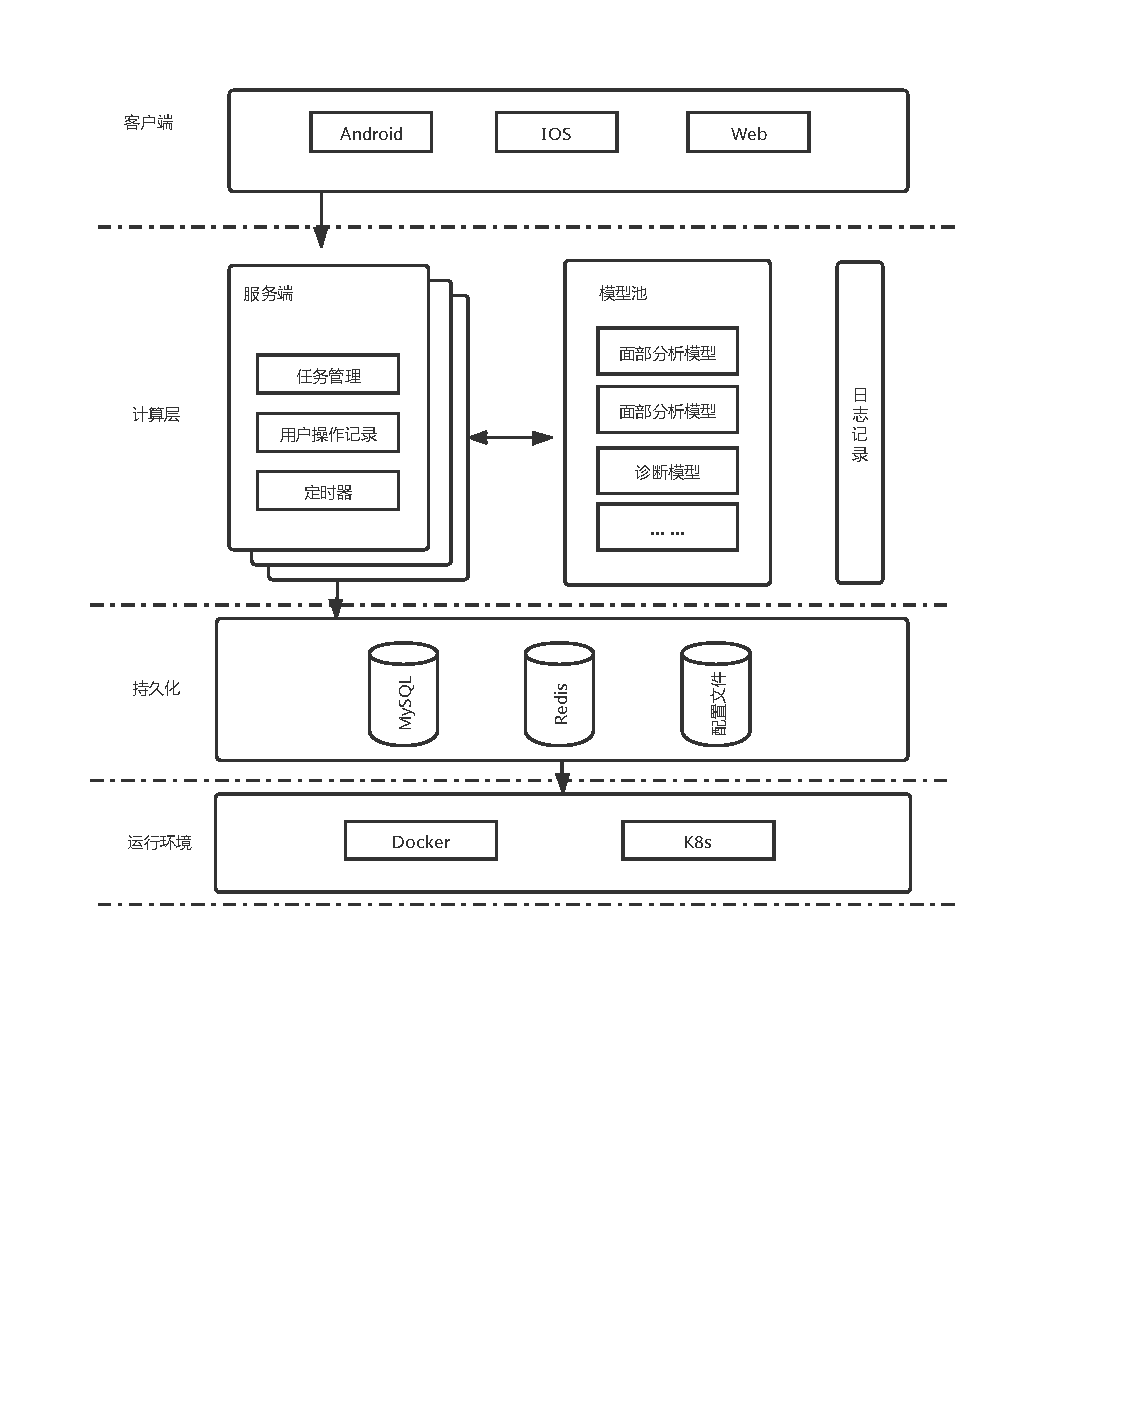
\includegraphics[width=15cm]{images/system2.pdf}
    \caption{跨平台系统设计}
    \label{fig:system}
\end{figure}

如图\ref{fig:system}所示,系统整体运行在容器环境下,使用Redis和MySQL作为持久化工具,主要分为三部分:服务端和客户端,算法模型通过容器的方式(docker\footnote{https://www.docker.com/}、kubernetes\footnote{https://kubernetes.io/})服务化成模型池。

客户端包括Android、IOS和Web平台的客户端,与用户交互密切相关,负责用户面诊的流程已经数据上传,通过请求服务端的接口完成面诊和记录用户的操作信息;
服务端通过调用模型池的相关服务,为客户端提供接口服务。其中静态页面的服务通过nginx提供,服务端则使用Django作为开发框架;
模型池是指在容器环境下通过容器服务化的方式下所有可用的模型服务的统称,为服务端提供计算服务,完成面部图片分析,舌部图片分析等任务。
大多数模型格式为二进制可执行文件或者本地模型文件的形式,为了方便服务端调用,需要对其进行服务化。

服务化指的就是将算法模型,打包成可调用的服务。其中本文的模型服务化通过Flask框架实现,每一个模型的服务都可以对应服务端中的一个计算任务。
服务端在任务管理模块中定义了任务的输入输出格式,模型池中的服务只要保持格式一致就可以保证服务端能够顺利调用对应的模型服务。

一次诊断的大致流程如下:用户通过客户端,上传图片或者回答问题,客户端则向服务端发起请求。
服务端收到请求之后,进行任务分配,对分配到任务的服务端实例,调用模型池中对应的模型完成特征提取或诊断打分,同时将数据持久化到mysql和硬盘中,然后把结果返回给客户端。
客户端收到服务端的结果后,进行结果的展示。

\section{模型池}
% 什么是模型池
本文提出一个模型池的概念,模型池由多个独立可用的模型服务构成, 通过http 接口调用完成和服务端的交互进行任务处理。

% 为什么要模型池
提出模型池的概念,是为了将模型和服务端独立,方便以后添加或删除模型。同时,将模型独立做成服务,可以动态增加模型运行的实例个数,提高计算能力和稳定性。

\begin{figure}[h]
    \centering
    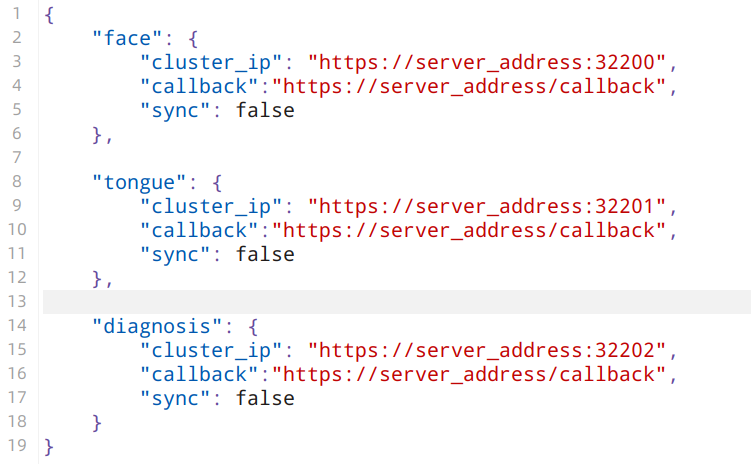
\includegraphics[width=15cm]{images/services.png}
    \caption{模型池配置}
    \label{fig:services}
\end{figure}

% 如何实现的
如图\ref{fig:services}所示,模型池维护一个<模型类型, cluster ip> 的映射,记录可用的模型和调用地址, cluster ip是由k8s(kubernetes)提供的集群调用地址。记录通过json文件的格式,记录在本地文件中。
其中sync参数代表是否同步返回结果,如果设置成异步返回,则通过调用callback地址将结果回调给服务端。


\subsection{模型服务化}
为了方便模型管理,我们需要将模型和客户端服务端独立出来,打包成独立可运行的服务。

docker和k8s是容器化解决方案和容器编排工具,能够很方便地实现这个需求。

模型服务使用docker进行打包,通过k8s管理多个模型高实现可用。服务端通过k8s提供的cluster ip进行调用,这样能保证在大量用户同时请求模型服务时,某个模型服务如果出错,集群中的其他模型服务能够响应请求。

为了减少服务之间读写的竞争,模型池中的服务只进行计算,不进行对mysql和redis的读写,结果的持久化由服务端完成。

服务化的过程是通过Flask\footnote{https://palletsprojects.com/p/flask/}框架建立一个Http的服务,把特征提取模型打包成服务。每个特征提取服务,接受http的请求,对传过来的图片进行特征提取。
模型的计算能力如 表\ref{tab:face-feature}, 表\ref{tab:tongue-feature}, 表\ref{tab:diag-feature}所示。

基于在云中医技术探针工作的基础上, 目前现有两类已实现的模型,特征提取模型(面部和舌部两种)和诊断打分模型,分别有对图片进行特征提取和对特征进行打分的能力。
特征提取模型对用户输入的特征(面部或者舌部图片)进行特征提取,而诊断打分模型,由一系列规则组成,定义了每一个特征对最终的打分输出影响的规则。

由于模型中的算法来自云中医,不属于本文的工作,因此接下来只介绍模型的输入输出的功能,算法的具体实现不多做介绍。




\subsection{脸部特征提取模型}

\begin{table}[h]
    \centering
    \begin{tabular}{lll}
        \toprule
        特征          & 特征描述     & 特征内容 \\ 
        \midrule
        faceDetectRes & 人脸   & 0:未检测出人脸,1:成功检测出人脸  \\
        faceColor     & 面部颜色 & 0:面白,1:面黑,2:面红,3:面黄,4:面青,5:正常 \\
        faceGloss     & 面部光泽 & 0:有光泽,1:少光泽,2:无光泽\\
        lipDetectRes  & 嘴唇   & 0:未检测出嘴唇,1:成功检测出嘴唇\\
        lipColor      & 嘴唇颜色 & 0:淡白,1:淡红,2:红,3:暗红,4:紫   \\
        \bottomrule
    \end{tabular}
    \caption{脸部特征提取模型输出}
    \label{tab:face-feature}
\end{table}

如表 \ref{tab:face-feature} 所示,脸部特征提取模型,输入为面部特征图片,输出有以下几个维度:

1. 是否检测到人脸(faceDetectRes):如果没有检测到人脸,则剩余所有维度无效,且取值为0。

2. 是否检测到嘴唇(lipDetectRes): 如果没有检测到嘴唇,嘴唇颜色的结果无效且取值必定为0。

3. 面部颜色、面部光泽(faceColor、faceGloss) : 面色和光泽是对预处理之后的图片,去除眼口鼻区域的图片进行面色和光泽信息提取的结果。

4. 嘴唇颜色(lipColor): 嘴唇颜色的结果从浅到深分别为淡白,淡红,红,暗红,紫。



\subsection{舌部特征提取模型}

\begin{table}[h]
    \centering
    \begin{tabular}{lll}
        \toprule
        特征 & 特征描述 & 特征内容 \\ 
        \midrule
        tongueDetectRes & 舌体 & 0:未检测出舌像,1:成功检测出舌像 \\
        tongueCrack & 舌裂纹 & 0:未检测到裂纹,1:成功检测到裂纹 \\ 
        tongueFatThin & 舌胖瘦 & 0:正常(瘦),1:胖舌 \\
        tongueCoatThickness & 舌苔厚薄 & 0:薄,1:厚 \\
        tongueCoatColor & 舌苔颜色 & 0:苔白,1:苔黄 \\
        tongueNatureColor & 舌质颜色 & 0:舌暗红,1:舌淡白,2:舌淡红,3:舌红,4:舌紫\\
        \bottomrule
    \end{tabular}

    \caption{舌部特征提取模型输出}
    \label{tab:tongue-feature}
\end{table}

如 表 \ref{tab:tongue-feature} 所示,舌部特征提取模型,输入为舌头图片,输入有以下几个维度:

1. 是否检测到舌体(tongueDetectRes): 如果没有检测到舌体,则剩余所有维度无效,且取值为0。

2. 是否检测到舌裂纹(tongueCrack): 舌裂纹是最终特征,剩余特征是否有效和该标志位没有关系。

3. 舌头特征(tongueFatThin、tongueCoatThickness、tongueCoatColor、tongueNatureColor): 包括舌胖瘦,舌苔的厚薄,颜色和舌质颜色。



\subsection{诊断模型}

\begin{table}[h]
    \begin{center}
        \begin{tabular}{lll}
            \toprule
            特征 & 特征描述 & 特征内容 \\ 
            \midrule
            healthScore & 健康分数 & 0-100 \\
            healthType & 是否包含某种体质 & {[}0, 0, 0, 0, 0, 0, 0{]} \\ 
            questionScore & 各种问题的体质得分 & {[}0, 0, 0, 0, 0, 0, 0{]} \\
            symCount & 各种体质症状个数 & {[}0, 0, 0, 0, 0, 0, 0{]} \\
            symNum & 总体体质症状个数 & 0-13 \\
            baseScore & 基本分数 & 0-100 \\
            phy & 体质结果 & 八种体质中的一种\\
            \bottomrule
        \end{tabular}
    \end{center}
    \caption{诊断打分模型输出}
    \label{tab:diag-feature}
\end{table}

% 原版的云中医应用中,只给用户暴露了健康分数和体质结果。

如表 \ref{tab:diag-feature} 所示,最终诊断打分模型的体质结果输出为 "阳虚","阴虚", "痰湿","瘀滞", "脾虚", "肾虚", "气虚", "健康" 中的一种,具体的特征说明如下:

1. 健康分数(healthScore): 打分的最终健康分数,由baseScore、symNum、questionScore计算而来。

2. 体质类型(healthType): 大小为7的数组,对应 "阳虚","阴虚", "痰湿","瘀滞", "脾虚", "肾虚", "气虚", "健康"。如果包含某个体质,对应位置的值为1。

3. 问题得分(questionScore): 一共有13个问题,每个问题都会影响最终体质的倾向得分, questionScore是所有问题的得分的累加。

4. 症状个数(symCount): 13个问诊问题中,对应有某个体质特征的症状的累加。

5. 总体症状个数(symNum): symCount的求和。

6. 基本分数(baseScore): 诊断任务中, healthScore = baseScore*p + 症状分数*q ,对应不同的症状个数,计算最终得分用的baseScore是不一样的。 
p和q是模型中预设的权重, 症状分数由问题得分计算而来。

7. 体质结果(phy): 和healthType对应,给出用户的体质倾向。

诊断打分模型的最终输出是健康分数(baseScore)和体质结果(phy), 其他的特征输出,是为了后续的算法可解释性做准备。


\section{服务端}

服务端使用基于Python语言的Django框架 \footnote{https://www.djangoproject.com/}实现,允许有多个服务端实例同时运行,共同处理用户发起的诊断任务,使用redis和mysql进行数据的持久化。
Redis \footnote{https://redis.io/}是基于内存的分布式数据库,在本系统中主要保存服务端可用节点的信息。
Mysql \footnote{https://www.mysql.com/} 是当前比较流行一个关系型的数据库,在本系统主要主要保存用户操作信息,任务信息等。       

服务端的主要模块如图 \ref{fig:server} 所示, 其中用户操作记录管理提供了网页端的管理界面,能够在线地对用户操作进行查询导出;任务管理为客户端提供了任务提交和结果查询接口,为客户端的面诊、舌诊、问诊提供支持。

系统通过设置定时器,定期地发送心跳包进行主从竞选,主节点会进行任务分配,主节点和从节点则对分配到的任务进行执行,调用模型池中对应的模型服务完成任务。


\begin{figure}[ht]
    \centering
    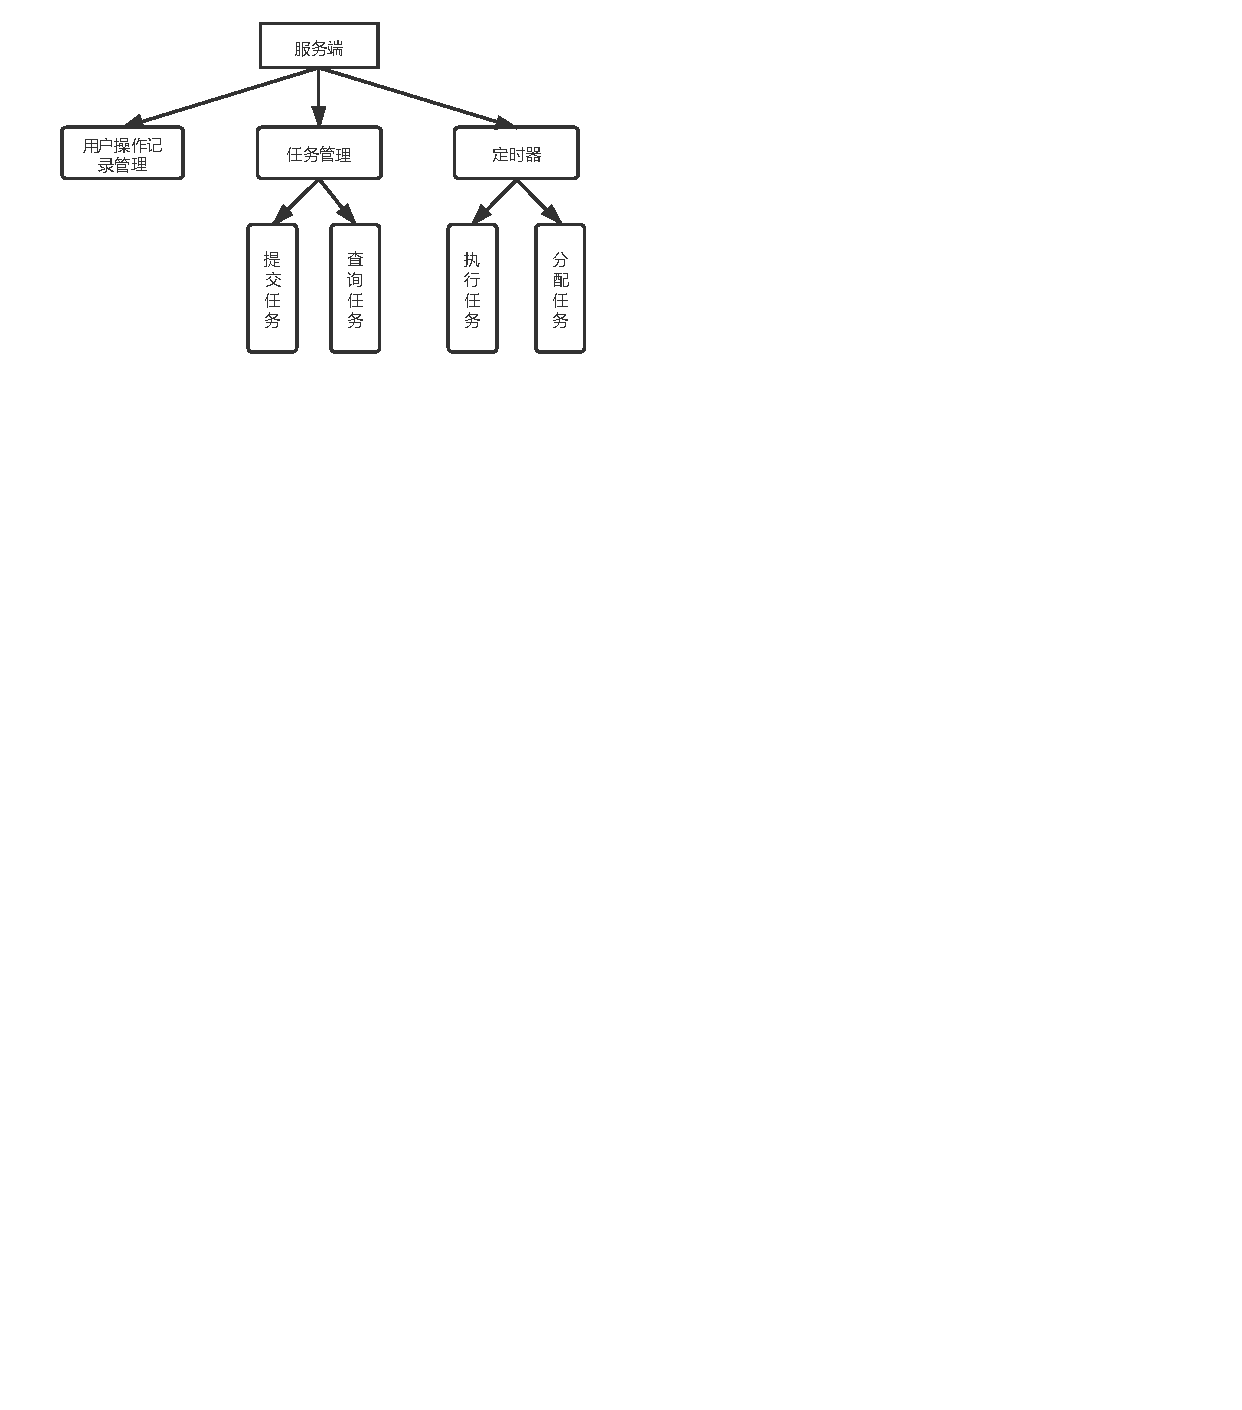
\includegraphics[width=12cm]{images/server.pdf}
    \caption{服务端主要模块设计}
    \label{fig:server}
\end{figure}


\subsection{用户操作记录管理}
为了方便后续的数据分析,我们需要采集用户的所有用户操作记录。客户端通过调用服务端接口将用户操作记录保存在数据库中,用户操作记录的数据库表的主要字段如表 \ref{tab:op_log} 所示:

\begin{table}[]
    \centering
    \begin{tabular}{lll}
        \toprule
        字段 & 类型 & 描述 \\ 
        \midrule
        id & int & 主键 \\
        user, & text & 用户唯一标识 \\ 
        device & text & 所用设备信息 \\
        op & text & 操作名 \\
        info & text & 操作信息 \\
        createTime & datetime & 创建时间 \\
        updateTime & datetime & 更新时间\\
        \bottomrule
    \end{tabular}
    \caption{用户操作记录表}
    \label{tab:op_log}
\end{table}


其中,user字段用于标识用户,默认使用用户手机号作为唯一标识,要求用户进入系统前需要通过手机验证码进行登录。


而在后续的实验环节,为了方便用户跳转完成问卷,不需要用户进行登录,user字段采用的是wjx-问卷星id。

\begin{figure}[ht]
    \centering
    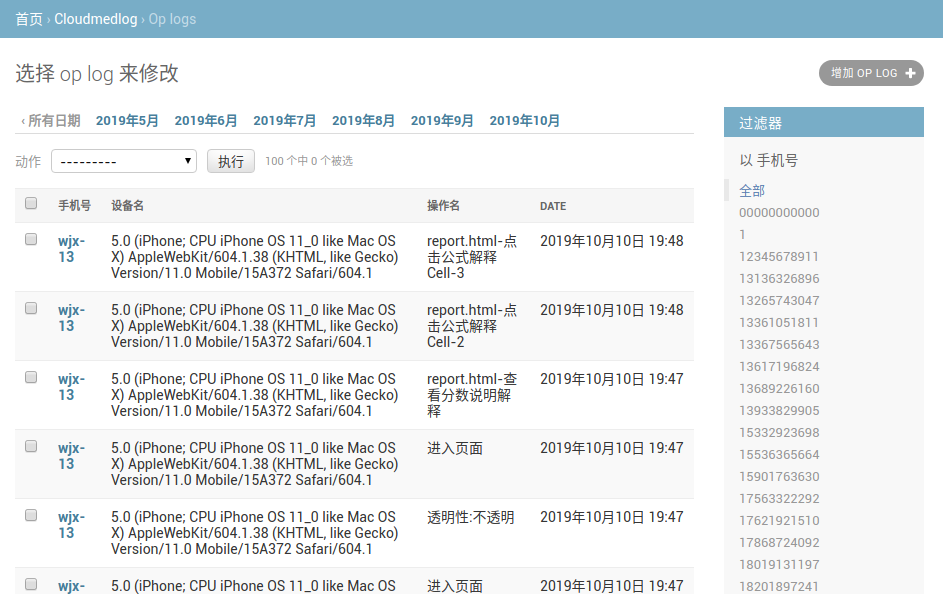
\includegraphics[width=12cm]{images/op_log.png}
    \caption{用户操作记录管理界面}
    \label{fig:op_log}
\end{figure}

\subsection{第三方问卷关联}
每次实验之前,根据实验的需求,可能需要先让用户填写一个问卷,收集必要的用户信息或者对用户进行评测;同样,在实验结束之后,也需要让用户填写问卷,收集用户反馈等。
在服务端重新实现问卷系统增加了工作量,我们通过接入第三方的问卷系统来实现,因此本系统需要对第三方的问卷系统提供对应的支持。


\begin{figure}[h]
    \centering
    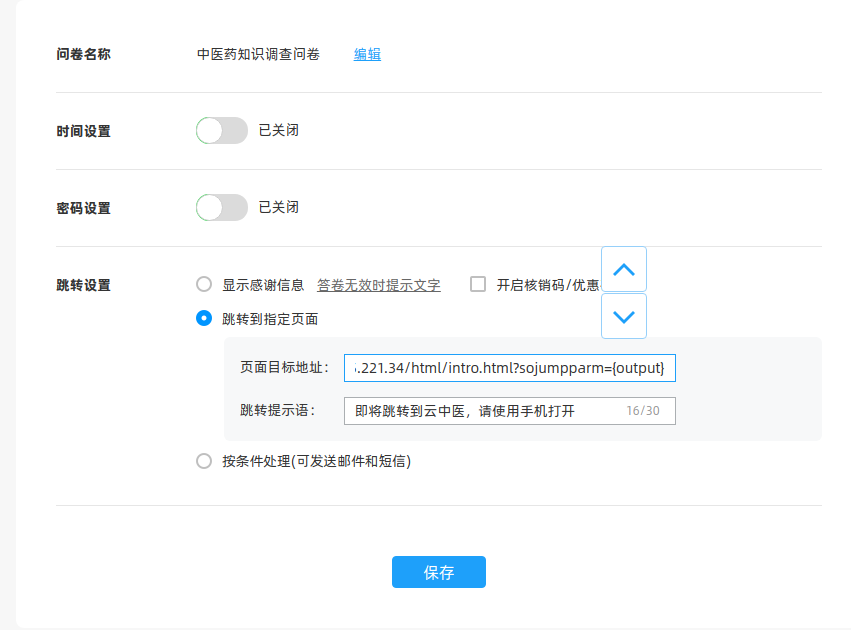
\includegraphics[width=10cm]{images/wjx1.png}
    \caption{第三方问卷系统跳转}
    \label{fig:wjx-ssojump}
\end{figure}

一次大致的实验流程为: 填写实验前问卷->进入实验平台完成实验->填写反馈问卷。在这个过程中,为了方便用户,我们需要通过特定的地址参数完成从问卷到实验平台完成自动登录。

如图\ref{fig:wjx-ssojump}所示,以问卷星为例,企业版的问卷星用户支持问卷完成后跳转到指定地址。指定的地址中可以带模板变量,如问卷的唯一id。
因此我们在系统登录页上只要判断是否存在该变量,如果存在则新建一个平台缩写+唯一id的用户名完成自动登录。


\subsection{任务处理}
一次用户诊断,服务端需要完成多个任务,目前支持的任务可以大致分类两类,计算任务和诊断任务。


\subsubsection{计算任务}
\begin{table}[]
    \centering
    \begin{tabular}{lll}
        \toprule
        字段 & 类型 & 描述 \\ 
        \midrule
        id & int & 主键 \\
        type, & int & 任务类型: 面部,舌部,诊断, 合并 \\ 
        extra & json & 模型相关信息 \\
        in & text & 任务输入 \\
        out & text & 任务结果 \\
        handler & text & 分配的服务端 \\
        status & int & 任务状态: 新建,已分配,处理中,失败,完成 \\
        createTime & datetime & 创建时间 \\
        updateTime & datetime & 更新时间\\
        \bottomrule
    \end{tabular}
    \caption{任务表}
    \label{tab:task}
\end{table}
计算任务对用户的输入进行计算,背后通过模型池中的模型来完成计算,如:面部特征提取任务,舌部特征提取任务,问诊任务。

服务端在收到用户提交的任务之后,会将数据存储到数据库的task表中,task表的主要字段如表 \ref{tab:task}所示:

1. type一共有四种取值,目前对应四种任务类型:面部特征提取任务,舌部特征提取任务,诊断任务和合并任务。

2. in为任务的输入,其中面部特征提取和舌部特征提取任务需要的输入为图片,通过Base64编码序列化为json对象,保存在in字段中。

3. out为任务的执行结果,在模型池的服务完成计算之后,服务端将任务执行结果保存到out字段,同时更新任务的状态。

4. handler保存当前任务是由哪个服务端在负责处理。

5. extra通过json格式存储模型相关信息,如分类任务,如体质判别,输出的7中体质的中文名称,保存在extra中。


\subsubsection{诊断任务}
% 合并任务只有前置任务,没有后置任务,它是整个任务调度流程中的最后一个任务。合并任务的主要功能是在所有计算类型的任务完成后,对计算出来的结果进行合并。

% 合并任务的触发时机,是在合并任务的所有前置任务完成之后。合并任务的合并流程如下:

诊断任务的执行逻辑在服务端实现,不在模型池中有对应的模型。 诊断算法的输入为每个任务的结果,输出为体质得分,健康分数。

在各类任务完成之后,诊断任务通过从redis或者mysql中获取当前已完成任务的结果作为输入,完成最终的诊断。 
诊断任务的内部实现是有一套规则系统组成,定义了每一个任务的输入,会对最终的输出产生怎么样的影响。

在该模式下,本地系统可以比较方便的添加新的模型: 在一个新的模型添加之后,只需要在规则系统中,添加一条新的规则即可完成模型的接入。

诊断流程具体如图 \ref{fig:sketch} 所示:

\begin{figure}[ht]
    \centering
    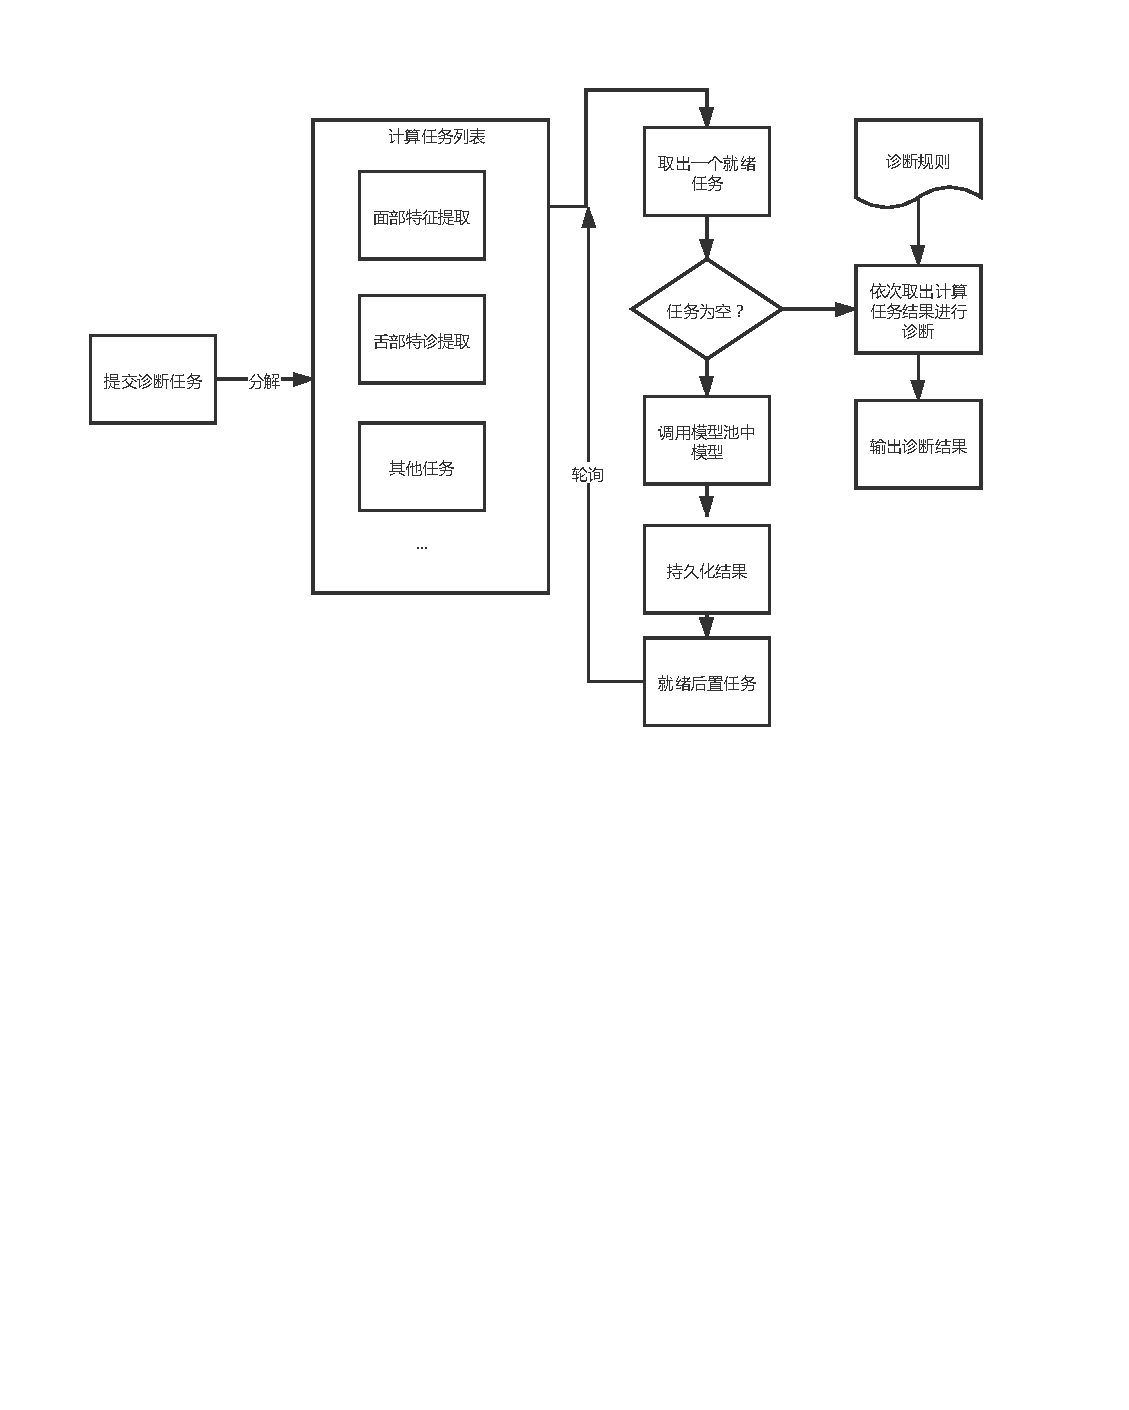
\includegraphics[width=12cm]{images/sketch.pdf}
    \caption{诊断流程}
    \label{fig:sketch}
\end{figure}

用户在提交诊断任务之后,服务端会将诊断任务分解成多个小的计算任务,其中包括面部特征提取,舌部特征提取以及其他相关的任务。任务分解的目的是降低单个服务端实例的计算压力,将任务计算分发到多个服务端,提高计算速度。
同时分解后的任务结果都保存在mysql数据库中,便于后续算法透明性暴露中间结果给用户。
在任务分解之后,通过轮询选出其中一个未完成的任务,调用相关服务完成计算;如果计算任务事先已经完成计算,或者经过轮询已经完成所有的任务,则通过规则系统,取出计算任务的结果进行诊断。



\subsection{任务分配}
%为什么要这样做?
为了实现服务的稳定性,服务端支持同时开启多个实例,即多个服务端同时处理任务。
同时考虑到性能,服务端设计为读写分离的架构:每个实例都可以读取任务列表,处理用户的任务,但只有主节点有任务分配的权限。


\subsubsection{主从节点}
% 为什么要这样做
为了屏蔽用户间的设备差异,让硬件较差的用户设备也能调用模型,本系统采用算法模型和客户端剥离的方案。
模型和客户端剥离则增加了服务端的计算压力,对系统稳定性要求更高。
因此服务端通过实现简单的读写分离和主从竞选的机制,使得服务端支持同时运行多个实例,提高稳定性和性能。


为了实现服务端的高可用,本文将服务端设计成允许多个实例同时运行,如果不做主从节点划分的话,每次有可用的任务时,所有节点都去抢占任务,会有大量锁的竞争的问题。
因此本文将每个实例的角色划分为主节点和从节点进行读写分离,不同节点的具体职责如下:

1. 主节点: 通过任务的id进行哈希,按照哈希进行任务的分配给各个节点,更新task表。分配任务时,只有主节点才有对任务表进行写操作的权限。

2. 从节点: 每个从节点每过一定的间隔时间,就会去读取任务列表,开始执行任务列表里属于自己的任务。

这样就保证了任务分配只由主节点去更新task表,而执行任务时,每个节点只会执行分配给自己的任务。

\subsubsection{角色竞选流程}
\begin{figure}
    \centering
    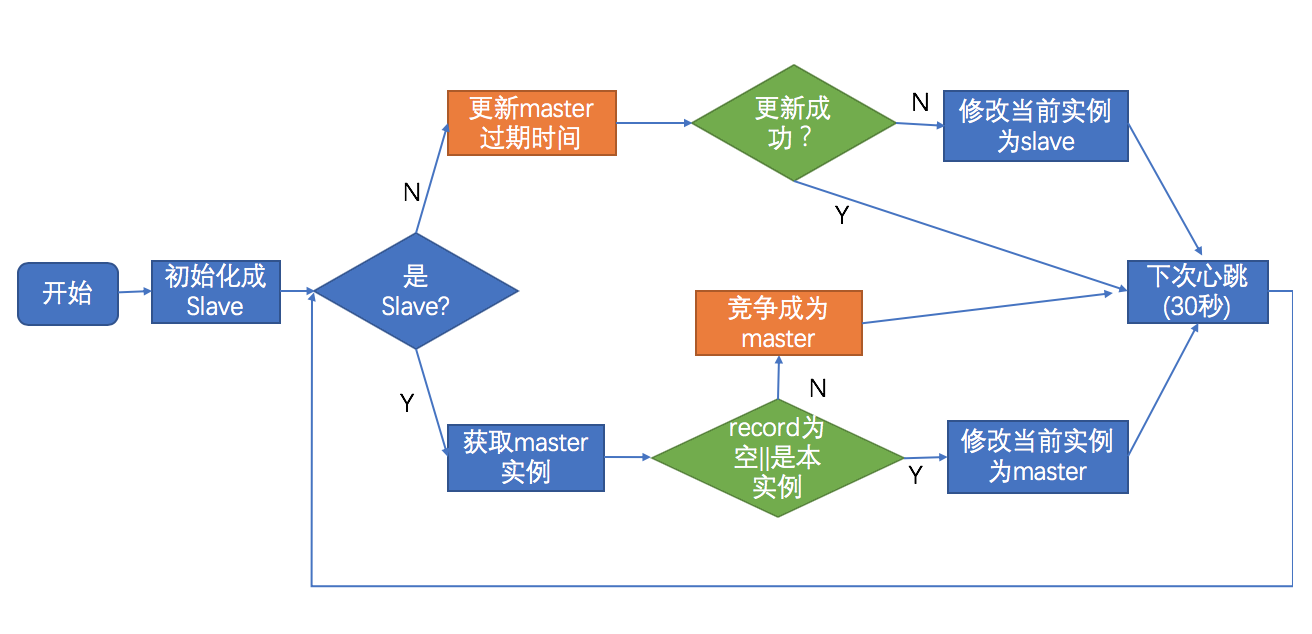
\includegraphics[width=10cm]{images/slave-master.png}
    \caption{服务端角色竞选}
    \label{fig:slave_master}
\end{figure}

服务端通过主从节角色分配的方式,同时运行多个实例来提高系统的响应速度,但多个实例同时运行也带来了系统稳定性的问题,如节点因为网络问题或者其他问题失效时,则需要通过心跳包探测节点存活。

服务端通过心跳包探活,主节点失效时,通过redis的分布式锁实现主节点的竞选。

每个节点在启动之后,会在本地把自己的角色默认设置成从节点。
然后每过一段时间,判断自己节点的类型,主从节点分别执行以下的心跳策略竞选主节点:

(1) 主节点:主节点每次心跳的时候,更新redis中主节点的过期时间。如果更新成功,等待下一次心跳; 
如果更新失败(更新失败可能是自己没有及时更新,导致redis里的主节点过期,主节点的身份被其他节点竞争到了),则把自己的节点类型设置成从节点。

(2) 从节点:从节点每次从redis里获取主节点的信息,如果主节点信息无效或者长时间没有心跳(默认设置为两轮心跳周期),则开始抢占竞选锁,尝试更新redis的信息让自己成为主节点;
如果redis的主节点信息已经是本节点,说明上一轮抢占成功,将本节点的角色更新为主节点。


\section{本章小结}
本章介绍了实验平台的方案选型到具体实现,其中实验平台被划分为模型池、服务端和客户端。
这样,客户端就与模型以及诊断细节实现了独立,只需要关注交互的部分。同时为了方便实验,服务端还提供了用户操作记录管理和问卷关联的功能,方便采集用户信息和后续分析用户行为。
客户端的具体实现和实验内容密切相关,不同的实验中客户端的具体实现不同,所以客户端的内容在下一章具体介绍。

% 5.交互实验
\chapter{交互实现及验证实验}

% todo: 介绍第四章完成之后,有了实验平台之后,可以利用实验平台对按照第三章的设计思路探索具体的设计应该如何实现

在第三章我们通过交互研究,发现了大量待解决的交互问题,并得出对应的设计思路有三条:支持可持续使用、系统可解释性、日常可用性。

% 根据设计思路,我们可以通过上一章实现的实验平台逐一进行交互实验。而通过增加系统可变性来支持用户的持续使用,需要大量相关的医学知识的相关数据库,实现起来需要较长的时间和大量的工作量,本章并没有完全实现支持持续使用的所有设计思路,而是只实现了前后结果对比,具体在后续的增加日常可用性的实验中介绍。

% 基于上一章节的工作,接下来的实验工作只需要利用实验平台的提供接口完成客户端原型便可开始实验。


% 本章的实验分别是探索如何增加日常可用性和系统可解释性的实验。 
基于上一章节的工作,接下来我们可以利用实验平台的提供接口快速完成增加日常可用性和系统可解释性原型的开发和实验。
同时,通过这两次实验,也间接验证了实验平台的稳定性和功能可用性。具体的实验内容如下:

\begin{itemize}
	\item 实验1:日常可用性。去掉了强制的操作流程,基于用户更大的自由度的思想,探索了如何实现解决用户日常可用性问题的新设计。

	\item 实验2:系统可解释性。我们通过添加解释来实现系统可解释性,探索了如何增强日常场景下面诊过程中的可解释及其效果,如面诊、舌诊、问诊、结果的解释,影响权重的解释以及通过实验探索添加解释的作用。
	
\end{itemize}

为了能够让用户顺利完成面诊的流程,原型系统需要提供图片预处理的功能帮助用户选取图片和裁剪图片,同时登录注册功能用于在日志中标识用户信息。其中,用户登录和诊断记录查看及图片预处理是各个原型系统通用的功能,健康诊断和健康报告在不同的原型中实现稍微有不同。因此接下来先介绍各个原型系统的通用功能,然后依次单独介绍两个实验。

\section{实验原型通用功能}
通用功能主要包括用户登录、诊断记录和图片裁剪等,采用MUI+AngularJS作为主要开发框架,结合大量插件完成具体实现。客户端通过调用实验平台提供的模型接口,让用户完成诊断的过程。

\begin{figure}[h]
    \centering
    \subfigure[用户登录]{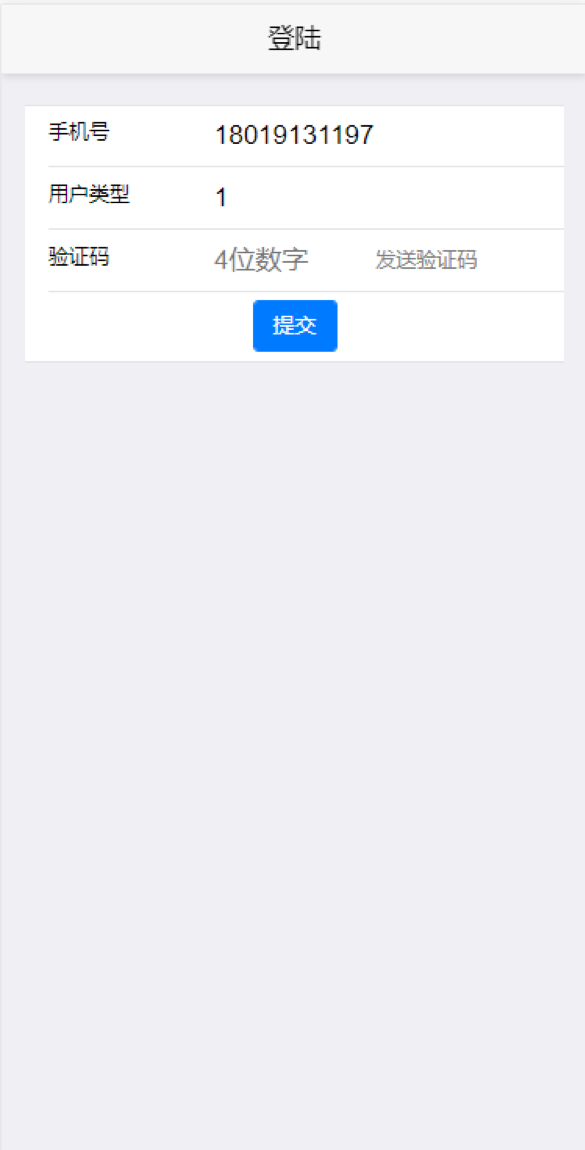
\includegraphics[width=4.5cm]{images/login.png}}
    \subfigure[诊断记录列表]{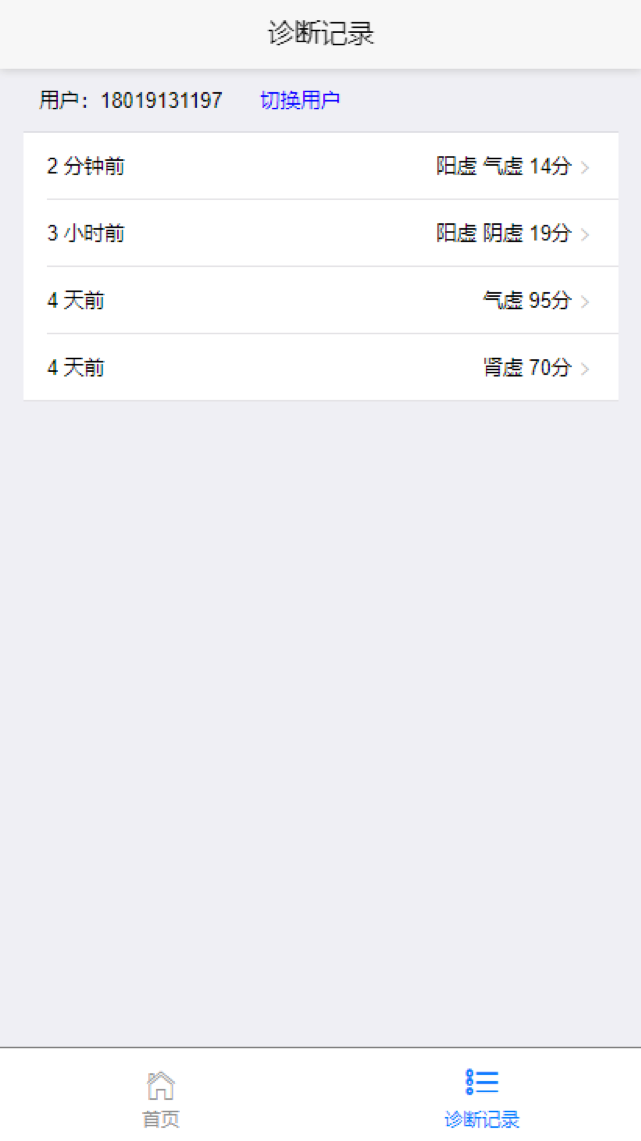
\includegraphics[width=4.5cm]{images/history.png}}
    \subfigure[图片裁剪]{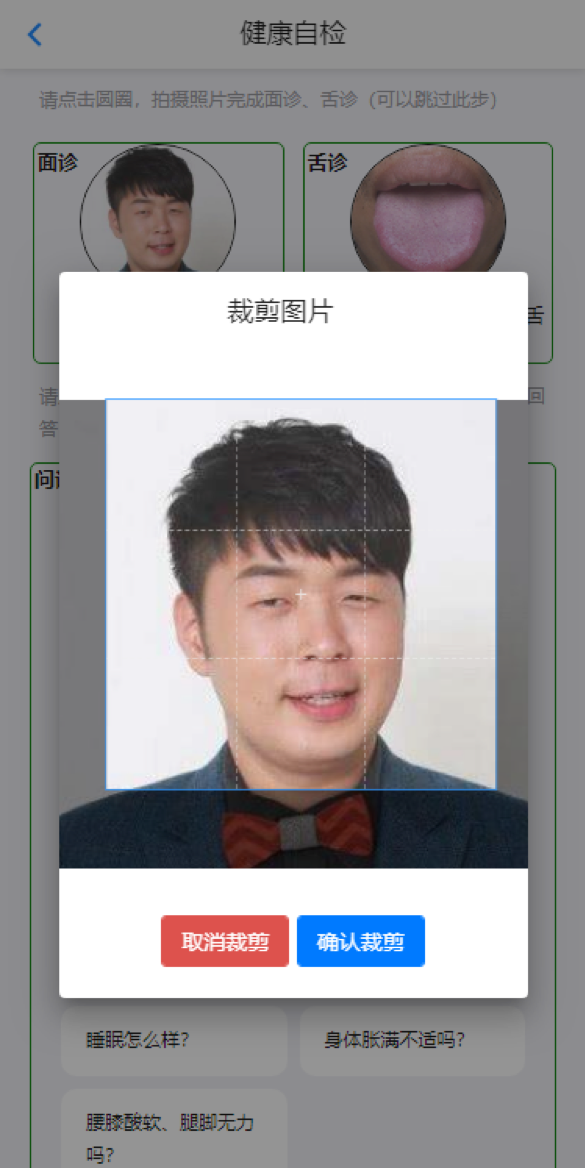
\includegraphics[width=4.5cm]{images/crop.png}}
    \caption{客户端实现}
    \label{fig:client}
\end{figure}

\subsubsection{用户登录}

当用户进入任意页面时,如果发现用户没有登录,会默认跳转到用户登录页面要求用户登录。

如图 \ref{fig:client} (a) 所示,用户登录时,需要输入正确的手机号才能通过手机格式验证发送验证码到手机上。

问了支持第三方问卷系统的跳转登录界面接收一个ssojump参数,用于判断是问卷来源。如果验证通过,则直接跳过登录进入首页。ssojump参数,是问卷星由问卷星平台提供的每一份问卷的唯一标识,是作为实验平台和第三方问卷系统关联的主要依据,因此客户端后续的日志,都需要带上ssojump的参数。

为了支持与第三方问卷系统的数据关联,日志记录时,上传的记录的附加信息为:问卷系统简写字母+问卷系统提供的标识。在本次客户端实现中,采用的是记录标识为wjx-ssojump的方式。

\subsubsection{诊断记录列表}

如图 \ref{fig:client} (b)所示,诊断记录页面,给出用户近期的健康变化的情况。用户可以点击诊断记录,进入当时的详细诊断结果页面。

\subsubsection{图片裁剪}

如图 \ref{fig:client} (c)所示,用户通过点击面诊或者舌诊,可以从相册选择或者通过拍照,上传自己的脸部或者舌头照片。
图片裁剪功能通过调用cropper.js\footnote{https://github.com/fengyuanchen/cropperjs} 实现,用户点击点击确认裁剪后,通过对图片进行base64编码上传到服务器的诊断接口,服务器调用模型池对应模型,拿到子任务结果。

图片裁剪可以帮助用户定位面部和舌头的位置,提高后续诊断的精度。用户点击确认裁剪之后,图片分析结果会直接显示。同时,如果没有识别到人脸或者舌头也会提示用户重新拍照。


\section{实验1:日常可用性设计实现与验证}

% 介绍原设计存在的缺点

% 在之前的研究中我们发现,目前的面诊交互设计在用户日常使用过程中存在以下问题:
在之前的研究中我们发现,目前的面诊交互设计在用户日常使用过程中存在以下具体的可用性问题:
\begin{itemize}
    \item 舌诊、面诊不能可选。与诊所环境不同,由于文化敏感性的问题,大部分中国人认为公共场合伸出舌头是非常不雅观的行为;部分用户也因为各种原因不愿意在非私人空间下拍自己的面部。这种设计对用户的日常使用产生了非常大的阻碍。
    \item 操作繁琐。在用户持续使用的时候,用户每次诊断和上一次通常没有太大的变化。每次让用户重复相同的操作不仅非常费时,而且影响使用的积极性。
\end{itemize}

根据第三章增加日常可用性的思路,本文同样用让用户参与设计过程的设计方法,通过实验平台在线更新设计原型的版本,邀请用户在日常使用的过程中参与迭代过程,最后实现了可用性设计原型。

\subsection{可用性设计原型实现}

\begin{figure}[h]
    \centering
    \subfigure[原型入口]{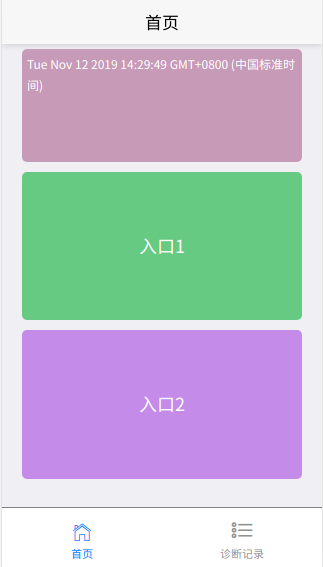
\includegraphics[width=4.5cm]{images/rukou.png}}
    \subfigure[新设计]{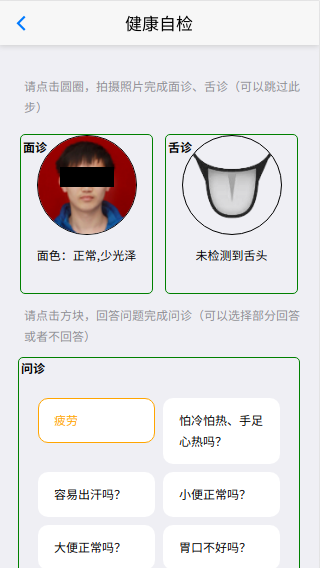
\includegraphics[width=4.5cm]{images/dialog1.png}}
    \subfigure[原设计]{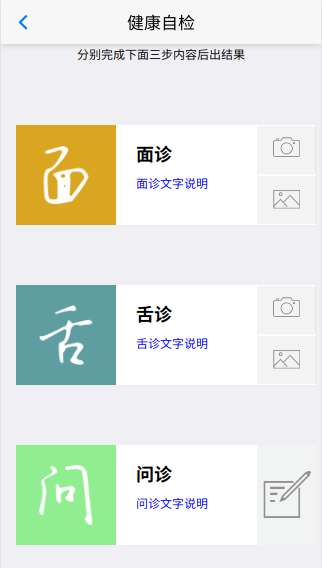
\includegraphics[width=4.5cm]{images/dialog2.png}}
    \caption{日常可用性验证实验}
    \label{fig:interface}
\end{figure}


在原始的云中医的设计中,用户在进行面部舌部拍照后,没有任何提示。具体的结果需要在用户一次回答13个问题之后,点击诊断才能知道面诊是否成功。
本文在实验平台上,实现了一个用于对比的原型系统, 如图\ref{fig:interface} 所示。在该原型系统的首页,有两个入口,新设计和原设计分别对应本文的设计和云中医的设计,两个设计的功能相同。用户在进入实验原型系统的首页之后,可以自由选择入口,进入对应的界面完成诊断。
新设计和之前版本的云中医界面不同的是,诊断界面不仅提供了面诊舌诊问诊的入口,同时会将面诊舌诊的照片和中间结果直接显示在当前页面,用户能对于自己当前身体情况一个直观的感受。

\subsubsection{迭代过程}
\begin{figure}[h]
    \centering
    \subfigure[设计1]{
        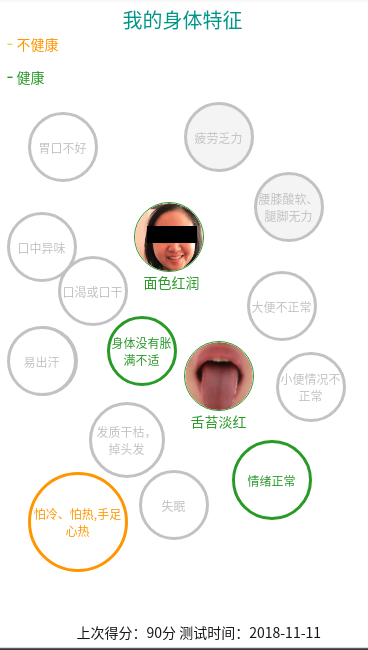
\includegraphics[width=3.5cm]{images/old1.png}
    }
    \subfigure[设计2]{
        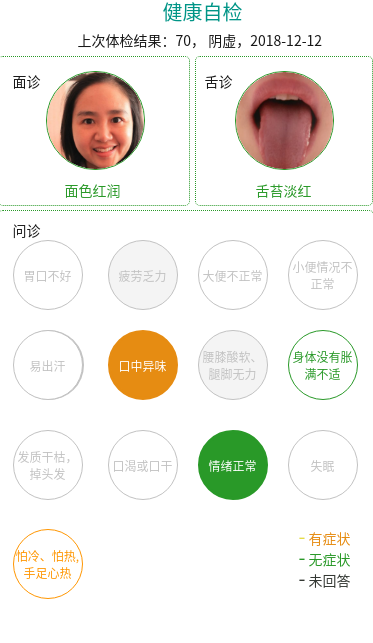
\includegraphics[width=3.5cm]{images/old2.png}
    }
    \subfigure[最终设计]{
        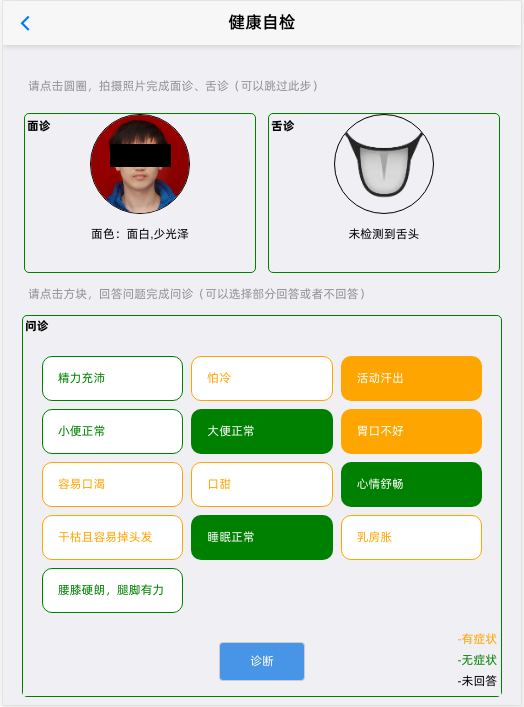
\includegraphics[width=4.5cm]{images/ui-1-1.png}
    }
    \caption{新设计迭代过程}
    \label{fig:diag_new}
\end{figure}
在进行可用性设计的过程中,原型系统经历了多次迭代。每次完成一版之后,我们会邀请小部分用户进行试用收集反馈并及时修改。
图\ref{fig:diag_new} 展示了部分中间的迭代版本和最终设计,其中设计1中的圆圈代表用户需要回答的问题,圆圈的大小代表影响的权重;
设计2简化了界面,统一了圆圈的大小;
最终设计进一步简化了界面元素,并把圆圈改为长方形,方便显示更多的提示信息。

\subsubsection{面诊问诊设计}

\begin{figure}[h]
    \centering
    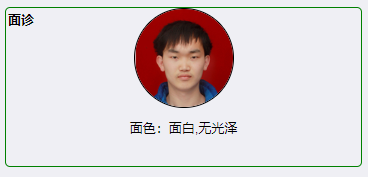
\includegraphics[]{images/diag_design.png}
    \caption{面诊元素设计}
    \label{fig:diag_design}
\end{figure}

根据日常可用性的设计思路,新设计简化了诊断的流程,面诊舌诊问诊在一个页面显示,并且所有的问题和操作都是可选的,不会出现必须要先面诊然后舌诊然后才能问诊的问题。其次,如图\ref{fig:diag_design}所示,新界面对面诊和舌诊进行了中间结果的反馈,面诊在用户拍照确认之后,会立即报告本次照片是否合格已经诊断的结果,用户不需要在点击诊断的时候才被提示照片不合格。

\subsubsection{问诊元素设计}
在问诊方面,新系统实现了最近一次记录保存,由于问题是可选回答的,所以用户只需要回答和自己上次的结果不一致的即可。

\begin{figure}[h]
    \centering
    \subfigure[上次回答有症状]{
        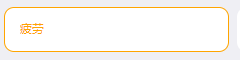
\includegraphics[width=6cm]{images/question/5.png}
    }
    \subfigure[上次回答无症状]{
        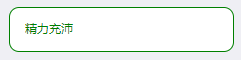
\includegraphics[width=6cm]{images/question/4.png}
    }
    \subfigure[本次回答有症状]{
        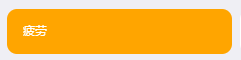
\includegraphics[width=6cm]{images/question/2.png}
    }
    \subfigure[本次回答无症状]{
        
\includegraphics[width=6cm]{images/question/3.png}
    }
    \subfigure[未回答]{
        
\includegraphics[width=6cm]{images/question/1.png}
    }
    \caption{问诊元素的状态}
    \label{fig:question_status}
\end{figure}

同时,如图\ref{fig:question_status}所示,我们对不同问题的回答结果进行了颜色的区分。有色实心代表本次回答,有色空心代表上次回答;橙色代表有症状,绿色代表回答的问题表现良好,没有症状;白色没有填充和边框,为黑字,代表未回答。实心颜色的代表的是用户本次有修改的问诊部分。

在方框内部的问题描述设计上,我们把默认的文字描述,显示为问题描述;一旦用户本次或者上次回答过该问题,则直接显示用户回答的结果。这样做的结果是,第二次用户点进来,就能看到上次的回答结果,这样能够对自己的身体情况有个快速的了解。


\subsection{实验设计}
为了验证本文设计的交互界面的有效性,本文设计了一个交互验证实验,用于验证客户端的实现是否解决了交互的可用性问题。实验流程如下:
\begin{enumerate}


    \item 通过海报(如图 \ref{fig:poster}所示,具体内容有对应的修改)和社交媒体,招募到了12位对中医感兴趣的志愿者参与了本次实验。

    \item 在招募到志愿者之后,我们通过实验平台的问卷关联功能,让每个用户填写一个志愿者的基本信息的问卷,然后单独给每位志愿者介绍我们这次实验的背景和这次实验的整个流程。

    \item 通知用户回家自由使用,我们可以通过实验平台的用户操作记录管理功能观察用户的使用日志,实验期间用户也可以随时反馈使用感受。

    \item 用户持续使用了大概两周之后,单独对每位用户进行深度访谈,通过录音的方式记录访谈数据。

\end{enumerate}

\subsection{实验结果}


\begin{figure}[ht]
    \centering
    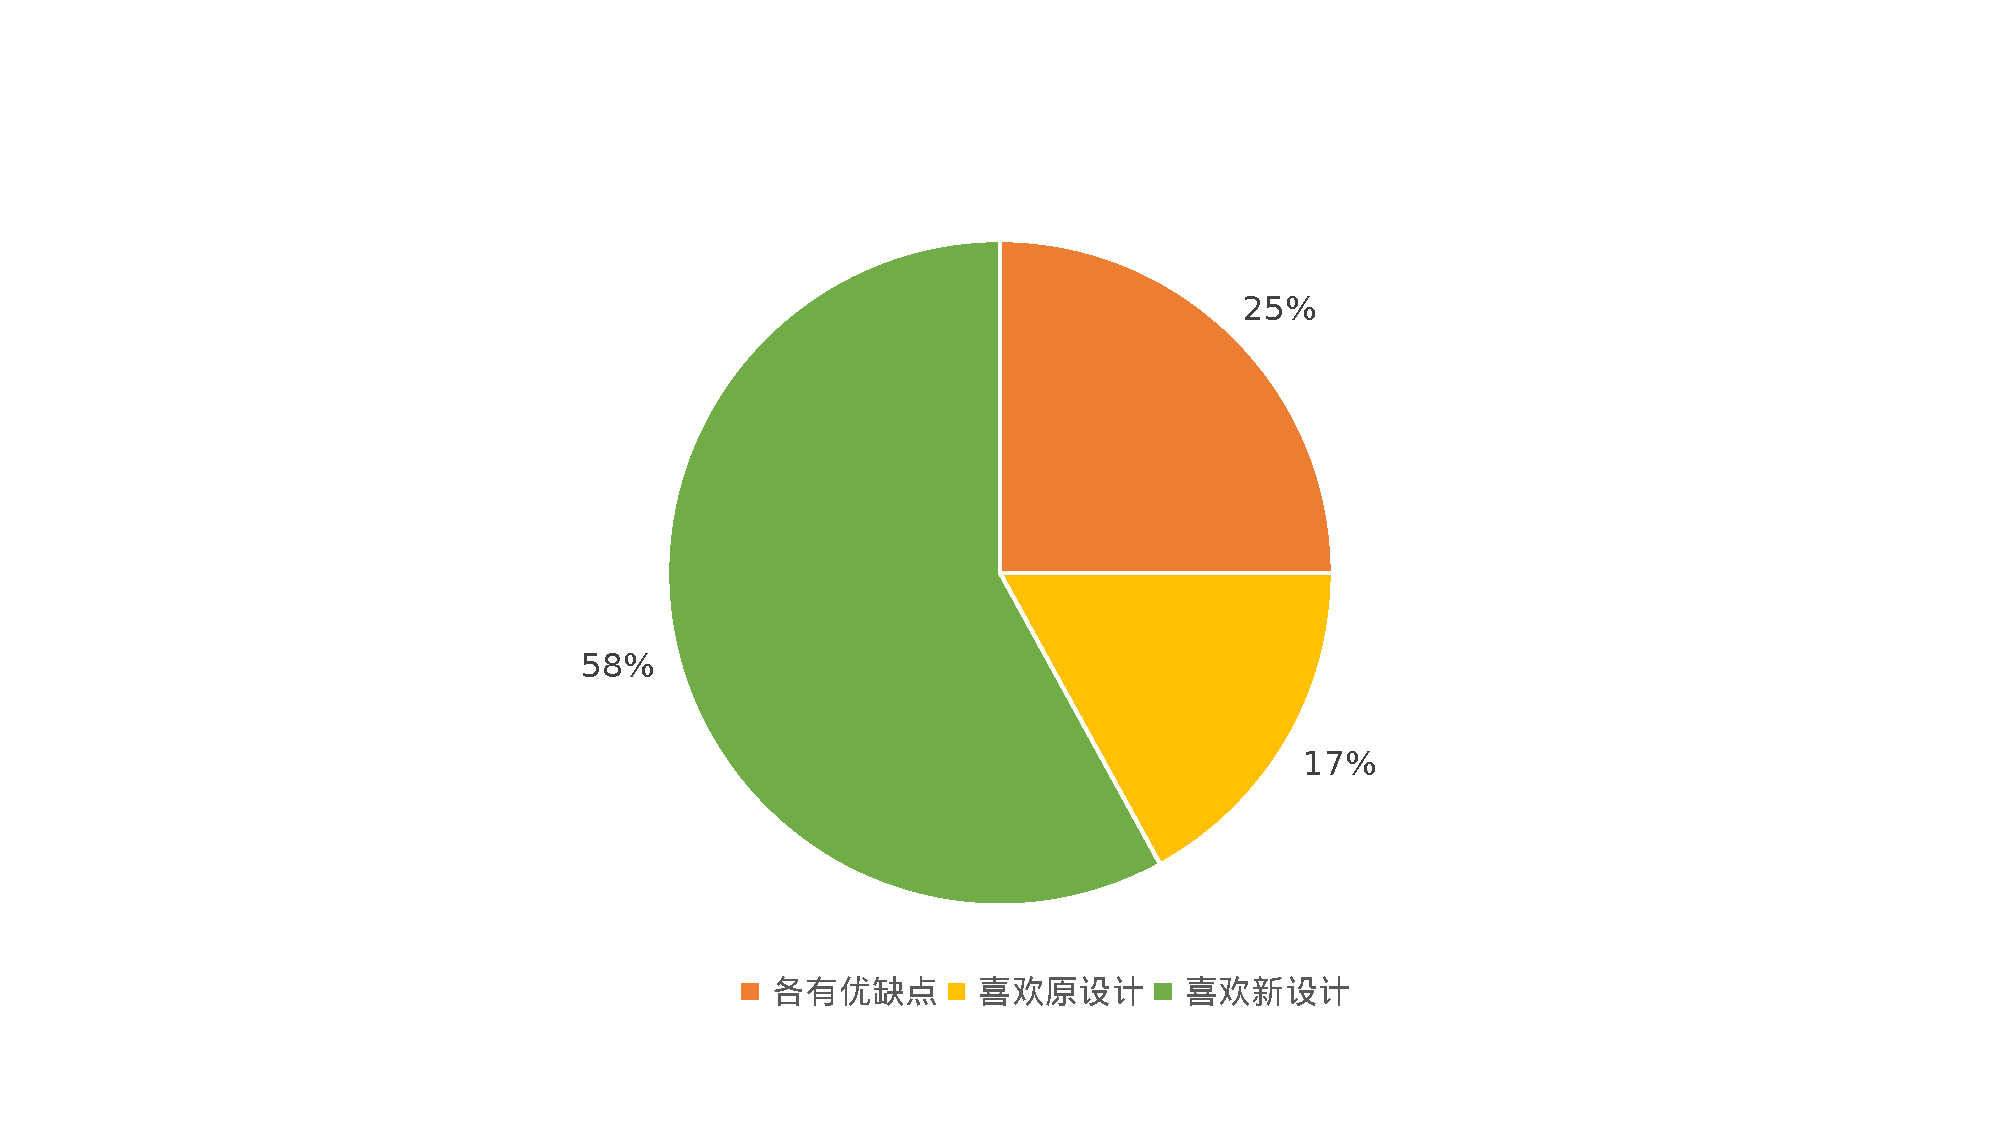
\includegraphics[height=8cm]{images/ui-exp.pdf}
    \caption{界面设计实验结果}
    \label{fig:ui-exp}
\end{figure}

如图 \ref{fig:ui-exp}所示,有少量志愿者选择持续使用原设计完成诊断,大部分用户更喜欢本文的新设计并且原因与用户调研的结果一致,而剩下部分用户觉得两种设计各有优缺点,具体原因如下:


\subsubsection{喜欢新设计}

和之前的用户调研的结果类似,新设计的确能够解决用户的部分日常可用性问题。

根据访谈数据,其中一位参与者认为新设计可以让他在日常使用时只完成自己想做的部分,更加方便:
\myfont{新设计方便,单独做某一块检测;给的指示不空洞;有针对性和选择性。}、\myfont{设计挺好的,感觉更方便一些。}

如我们的预期,新设计带来的可选择性同样在参与者的身上得到了反馈:
\myfont{新设计诊断透彻到位;可以选择性地做诊断,知道健康得分的构成,帮助了解中医知识,省时间。}、
\myfont{新设计操作更简单,有选择性,但是问诊的选项太少,涵盖不全。}

另一部分参与者虽然觉得新设计不好看,但是相对于原先缺乏可用性的设计,新设计基本解决了他的问题:
\myfont{虽然新设计界面丑,但原设计问诊很烦,而且新设计能实时显示舌诊结果。}、\myfont{想按照顺序回答问卷,新设计问诊界面不舒服;但是新设计的选择性检测比较方便。}


\subsubsection{喜欢原设计}
虽然新设计的设计理念是为了方便用户的持续使用,但也同样增加了界面的复杂度。

在选择使用原设计版本的用户中,其中一位参与者就认为新的设计对于他没有帮助而更喜欢一开始有模拟传统中医面诊流程感(先面诊舌诊再问诊)的原设计版本:\myfont{原设计界面好看,问诊流程有完成感,并不想知道具体的症状对应什么细节。}
而另一位参与者则认为问诊应该一次性全部完成,这样在操作上感觉更加连贯:\myfont{原界面设计更符合常规,问诊是连贯的,首页内容很清楚。}

本文提出的设计,虽然能够简化用户的操作,但是会让用户失去自己完成诊断的流程感。
新设计选择了一次性展示用户上次的诊断结果,但是本文的设计在内容丰富度和简单性的取舍下,选择了没有显示原有的问题和所有的选项,用户反馈这种代替用户做选择的方式让用户觉得没有参与感。
当用户希望得到更加准确的面诊结果的时候,繁琐的操作是可以忍受的。

\subsubsection{各有优缺点}
部分用户在实验过程中,两个设计的版本都在交替使用,也难以确定哪一个版本更加喜欢:
\myfont{界面设计更符合常规,问诊是连贯的,首页内容很清楚;新设计圆圈里的不同颜色有提示功能。}、
也有部分参与者反馈新设计并没有符合我们设计的预期,一次性展示所有的选项同样会让用户觉得所有的选项都必须选择:
\myfont{想按照顺序回答问卷,新设计问诊界面不舒服;但是新设计的选择性检测比较方便。}、
\myfont{新设计更方便,但一个一个问题点开很烦;原设计流程顺利,简单。}

\subsubsection{操作耗时对比}

\begin{figure}[ht]
    \centering
    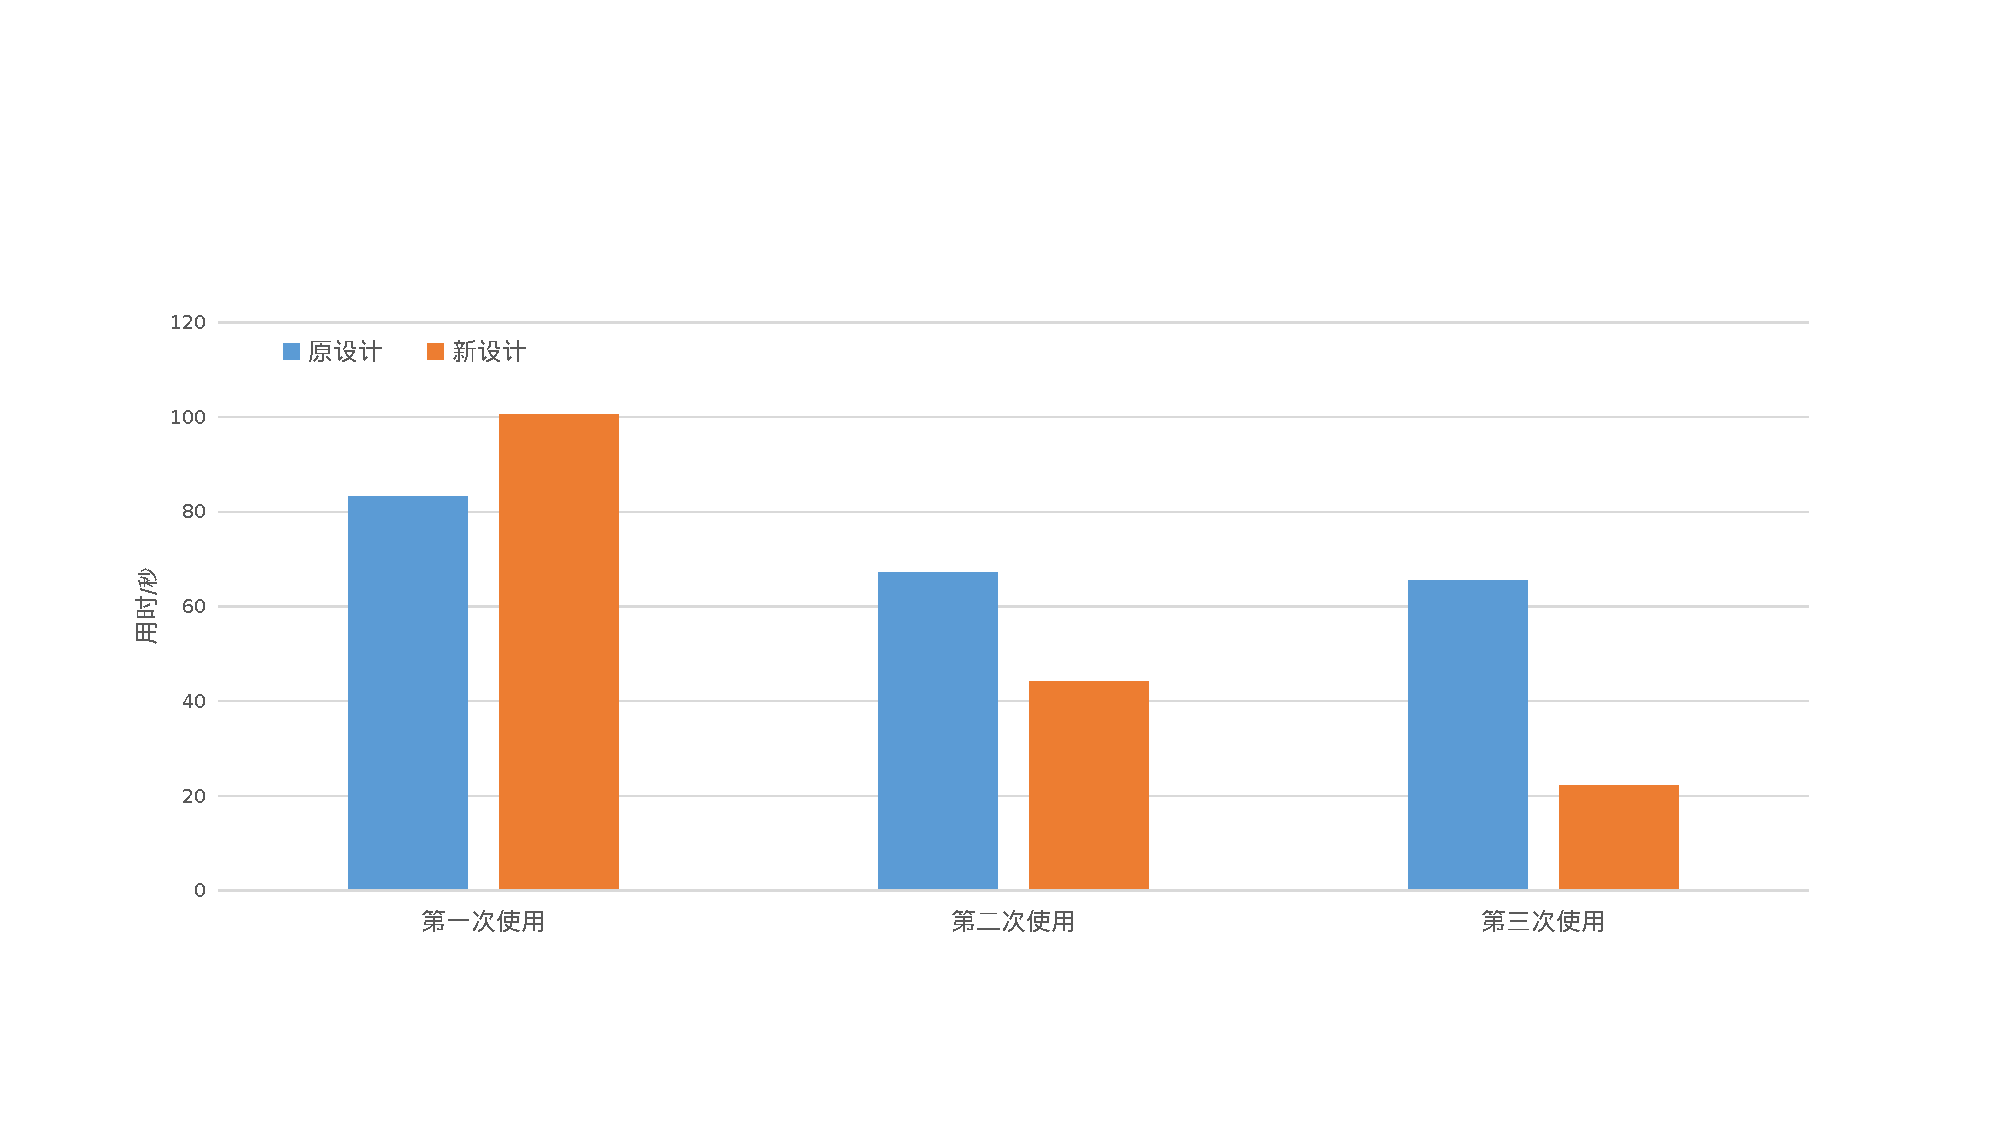
\includegraphics[width=13cm]{images/time.pdf}
    \caption{操作耗时}
    \label{fig:ui-time}
\end{figure}

由于大部分参与者在实验过程中使用系统进行诊断的次数不多,因此本文只通过部分用户的操作日志统计了前三次从进入诊断页面到完成诊断的时间,数据经过处理后的具体结果如\ref{fig:ui-time}所示:

\begin{itemize}

    \item 第一次完成面诊的操作耗时,新设计相比原设计对于用户来说需要更长的时间。如之前的参与者的反馈,新设计没有原设计直观和简单,由于界面相对复杂,因此用户理解后顺利完成诊断需要的时间也比较长。

    \item 在后续的第二次、第三次操作中,旧设计的操作时间在用户熟悉之后稍有降低,但是总体来说变化不大;新设计可以让用户直观的看到自己上次的面诊舌诊数据和问诊的选择,用户可以只选择完成有变化的部分实现快速诊断,完成一次操作时间大大降低。

\end{itemize}

\subsubsection{总结}
通过实验,我们发现新的设计在一定程度上的确解决了本文在之前提到的可用性问题。用户在日常使用的情况下能减少用户在完成诊断操作上花费的时间。
不过值得注意的是也有部分年纪较大的用户反馈新的设计过于复杂。总体来说符合日常可用性设计思路的预期,能够满足用户日常使用的需要。
% 没有依次做完面诊、舌诊、问诊的完成感,没有做到兼顾所有用户的需求。

\section{实验2:系统可解释性设计实现与验证}

% \cite{wang2019designing, lim2009and}

根据之前的用户调研的结果来看,当前系统存在以下问题:

\begin{itemize}
    \item 由于当前诊断和打分模型存在改进的空间,部分的用户对结果产生了怀疑或者对结果不理解的问题。
    \item 日常场景下,没有专业医护人员的帮助,普通用户由于缺乏对应的专业知识,对应用的理解还有很大的提升空间。
\end{itemize}

目前主要对提高用户对系统理解程度的方式一般是通过文字、可交互式元素或者可视化的方法描述来暴露算法置信度、暴露中间结果、提供当前数据和原始数据对比等实现\cite{wang2019designing, kocielnik2019will},其中文字化的描述适合对系统的背景、或者专业名词进行解释;暴露算法的中间结果以及置信度,能激起用户探索算法原理的好奇心以及提高对结果的容忍程度。

在这个理论的基础上,我们希望通过将模型的诊断过程对用户可见,并对结果进行解释,来提高用户的交互体验。
但是面诊系统在日常生活中的应用是一个全新的场景,需要解释的对象是什么,通过何种交互元素进行解释,仍是未知的问题。

% 系统可解释性可以通过解释算法置信度、算法中间过程等方式实现。因此我们在尝试系统中加入算法的解释性,提升用户的体验。

% 在这个基础上,我们希望通过将模型的诊断过程对用户可见,并对结果进行解释,来提高用户的交互体验。

% 虽然目前已有相关的对系统进行解释的方法\cite{wang2019designing, lim2009and},如通过解释算法的可信度,暴露原始数据和中间结果,以及通过图表等方式实现结果对比等,增加系统可解释性,可以提高用户的交互体验。

\subsection{可解释设计原型实现}

在第四章中本文详细介绍了目前技术探针中可用的模型,根据本文系统和模型的特点,解释在呈现的时候,实现的解释方法大致可以分为以下几种:

\begin{enumerate}
%  为什么要解释,文字解释的作用。
    \item 如图\ref{fig:face_diags}所示,结果中文字结果有提示、可以进行点击。如果用户点击了健康报告的分数,会通过弹窗通过文字描述进行详细的解释。

    \item 如图\ref{fig:question_weight}所示,通过雷达图的可视化方式直接显示对结果的影响,交互性比较强。 
    
    \item 如图\ref{fig:report_expalin_score}所示,通过可交互元素折叠列表对不同条件下的计算公式进行解释。
\end{enumerate}

用户在使用系统的过程中,需要经过面诊、舌诊、问诊等流程,最终得到诊断的结果。为此我们根据交互研究中用户反馈的问题,对用户完成一次诊断的中间流程以及最终的结果都进行了解释。

\subsubsection{面诊舌诊的解释}

\begin{figure}[htbp]   
    \centering
    \subfigure[不解释]{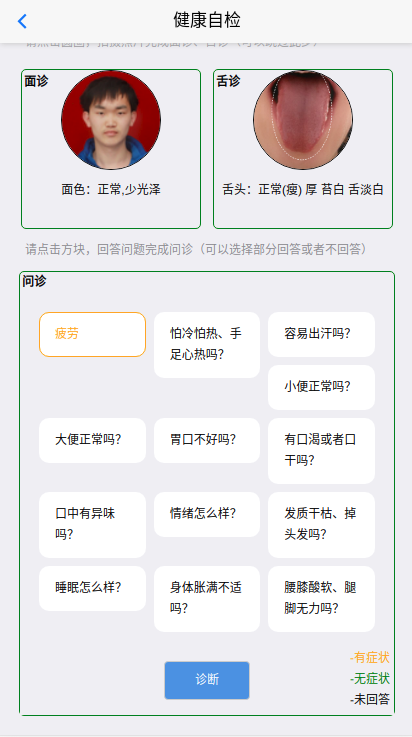
\includegraphics[width=4.5cm]{images/face_tongue.png}}
    \subfigure[解释]{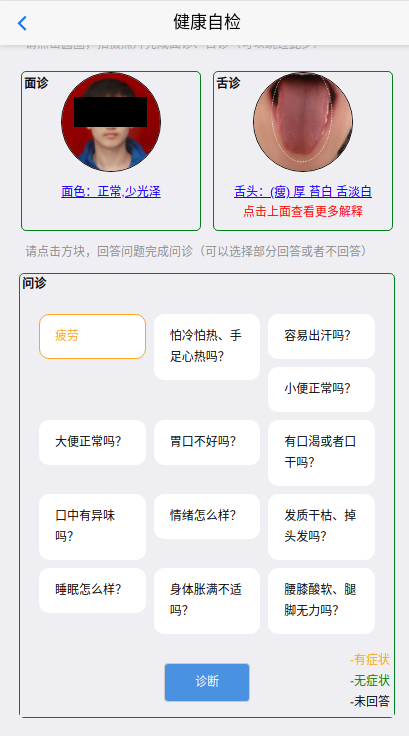
\includegraphics[width=4.5cm]{images/exp_face_tongue.png}}
    \subfigure[详细解释]{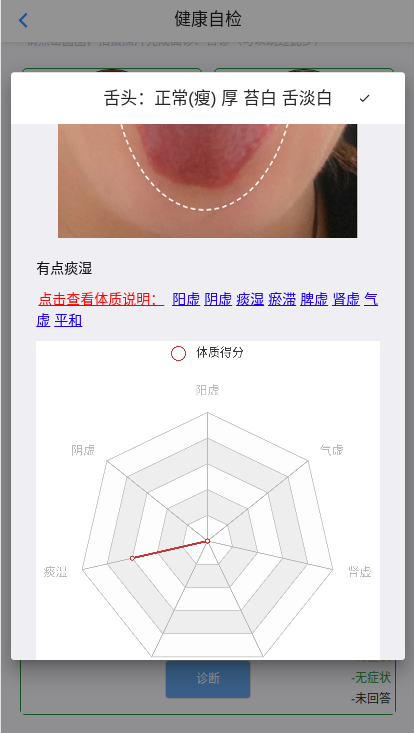
\includegraphics[width=4.5cm]{images/exp_tongue.png}}
    \caption{面诊舌诊的解释}
    \label{fig:face_diags}
\end{figure}

面诊和舌诊流程比较类似,都是通过分析面部或者舌部图片,得到分析结果,因此这两部分合并放到一起解释。
面诊和舌诊断添加解释主要体现在结果的解释,包括中间结果和对各种体质倾向的影响。
用户查看解释之后,能够大致了解本次拍照是否成功,并且知道目前面诊的结果,以及可能会对最终的健康报告造成哪些影响。具体如图 \ref{fig:face_diags} 所示:

(a) 没有解释的设计,只能看到结果。

(b) 有解释的设计,通过点击面诊或者舌诊结果,查看对结果的解释。

(c) 点开解释之后,系统会弹窗进行详细的解释,不仅可以看到当面诊断的中间结果,也能看到这次诊断的体质倾向得分。

接下来介绍该原型中各个解释的细节具体如何实现。


\subsubsection{问诊的解释}

\begin{figure}[htbp]
    \centering
    \subfigure[不解释]{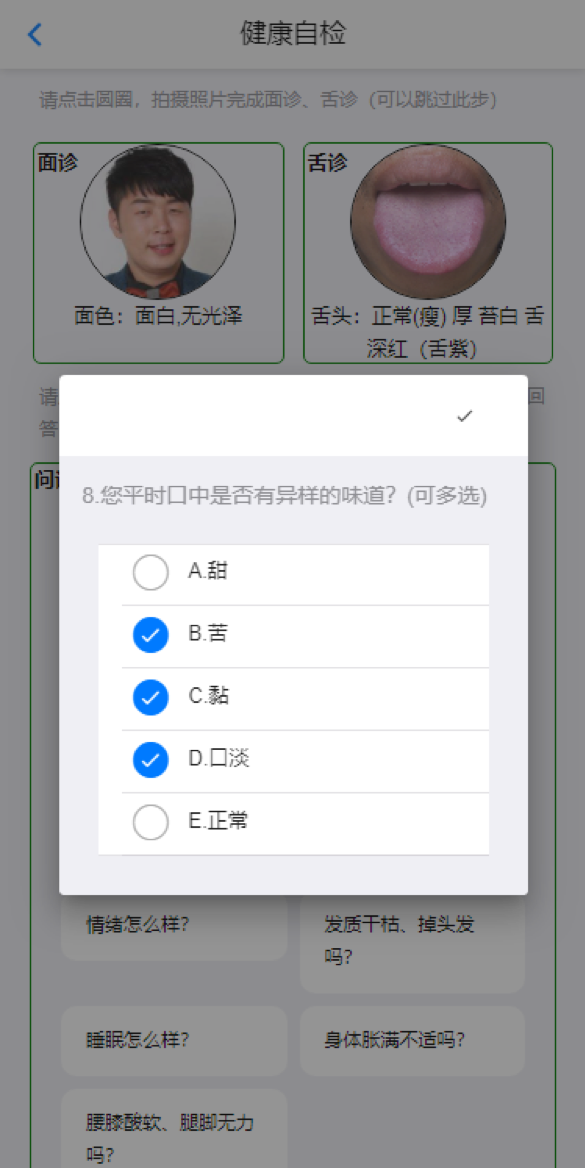
\includegraphics[width=5cm]{images/questions.png}}
    \subfigure[解释体质术语]{
        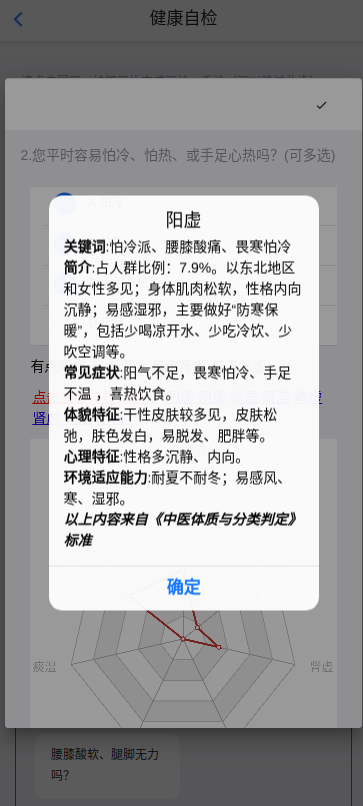
\includegraphics[width=5cm]{images/exp_phy.png}
    }
    \caption{问诊的解释}
    \label{fig:questions}
\end{figure}

问诊的过程中解释的主要实现,是通过对体质的专业术语和每个答案对结果的影响进行解释,具体实现如图 \ref{fig:questions} 所示:

(a) 不解释的设计,用户回答问诊问题之后,没有任何提示或者解释。

(b) 有解释的设计,用户在进行问诊过程中,可以立即看到每个答案对结果的影响,通过下方的雷达图显示了影响的体质倾向类型和具体的数值。
雷达图的更新是实时根据用户的选择进行更新的,用户可以通过点击不同的选项查看不同选项对应的雷达图。

(c) 点开体质的解释之后,会通过弹框的方式,对中医术语中,各种体质的解释。对于体质内容的解释文字引用自 《中医体质分类研究》标准\cite{王琦20099}。


\subsubsection{诊断结果的解释}
\begin{figure}[htbp]
    \centering
    \subfigure[不解释]{
        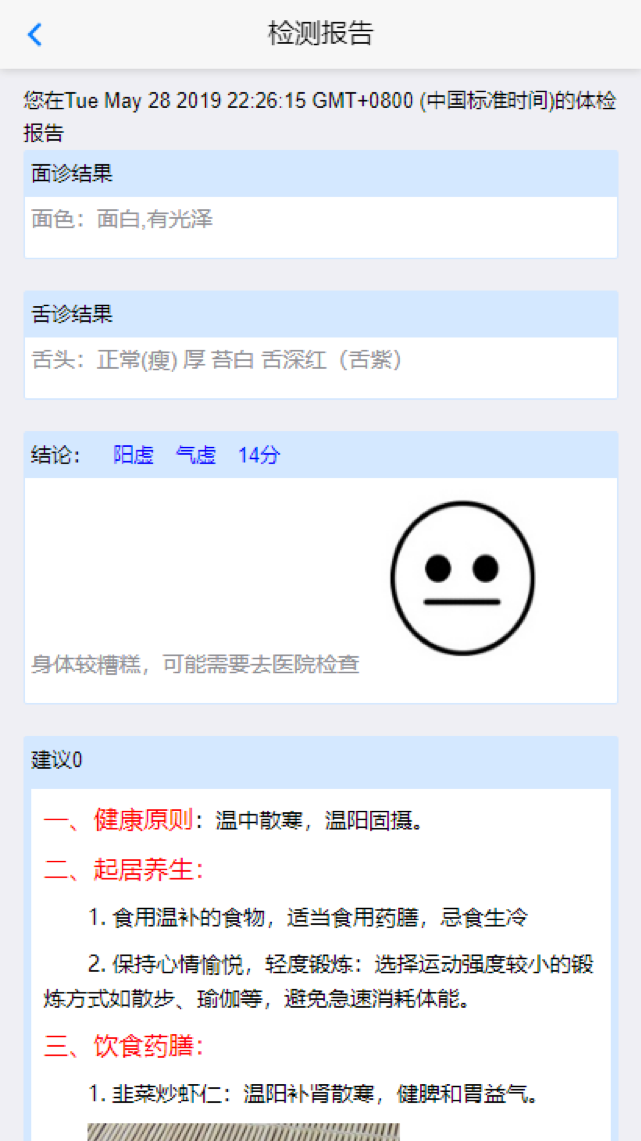
\includegraphics[width=4.5cm]{images/report.png}
    }
    \subfigure[解释]{
        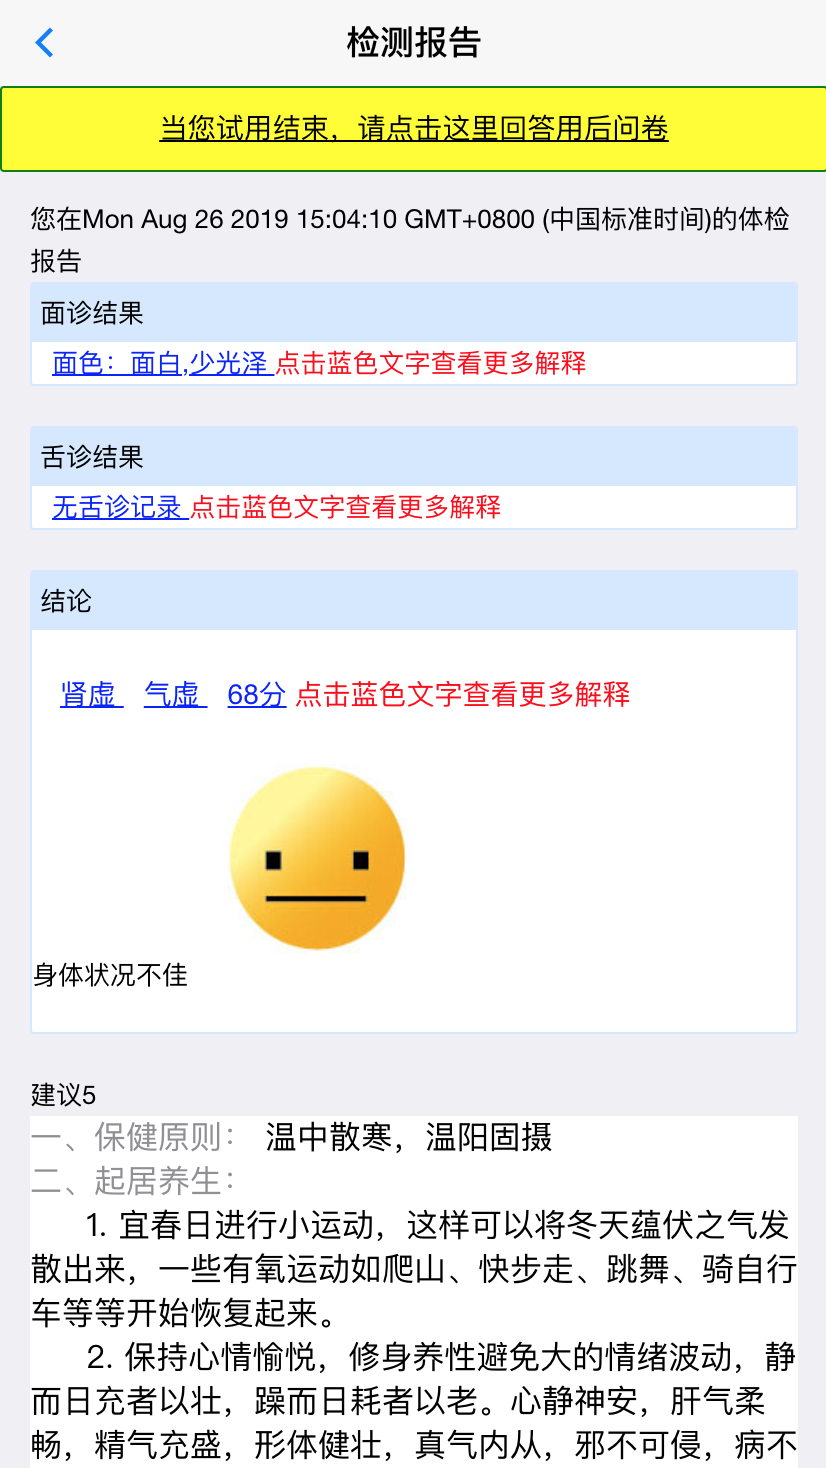
\includegraphics[width=4.5cm]{images/report3.png}
    }
    \caption{诊断结果的解释}
    \label{fig:exp_result}
\end{figure}

诊断结果的解释主要是对结果的判断依据和相关原理进行解释,具体如 \ref{fig:exp_result} 所示:

(a) 在没有解释的设计中,用户在诊断结果页面,可以看到自己的健康分数和体质结果,并且会在后面给出对应的养生建议和实践,但是给出的结果是不可点击的;

(b) 在有解释的设计中,用户可以点击诊断结果,包括面诊结果、舌诊结果,体质、健康分数。用户点击之后,可以通过之后的弹框,看到详细的解释,如点击健康分数之后,可以了解这个分数是根据哪些指标,通过哪一个算法计算过来的。

从\ref{fig:exp_result} 中我们可以看出有解释的设计中,用户点击结果后,会通过弹框解释结果。可以点击查看的结果的解释有:面诊舌诊结果的解释,健康分数的解释,体质的解释,接下来分别介绍如何实现。



\subsubsection{健康分数的解释}
问诊结果的解释主要是对用户解释诊断结果是如何计算,以及那些问诊的问题对结果有影响,影响程度多少。

\begin{figure}[htbp]
    \centering
    \subfigure[相关问题]{
        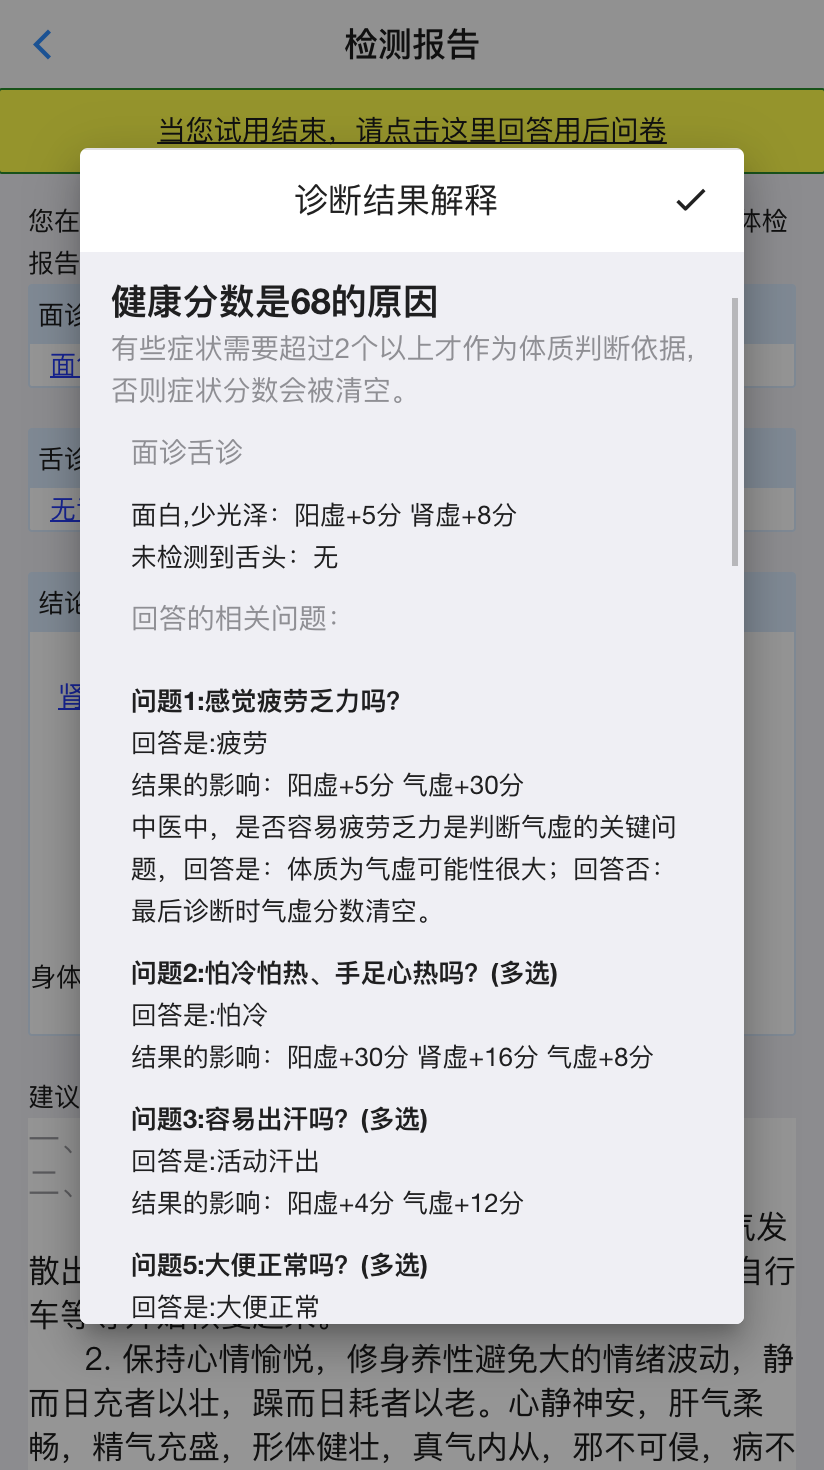
\includegraphics[width=4.5cm]{images/report7.png}
    }
    \subfigure[雷达图]{
        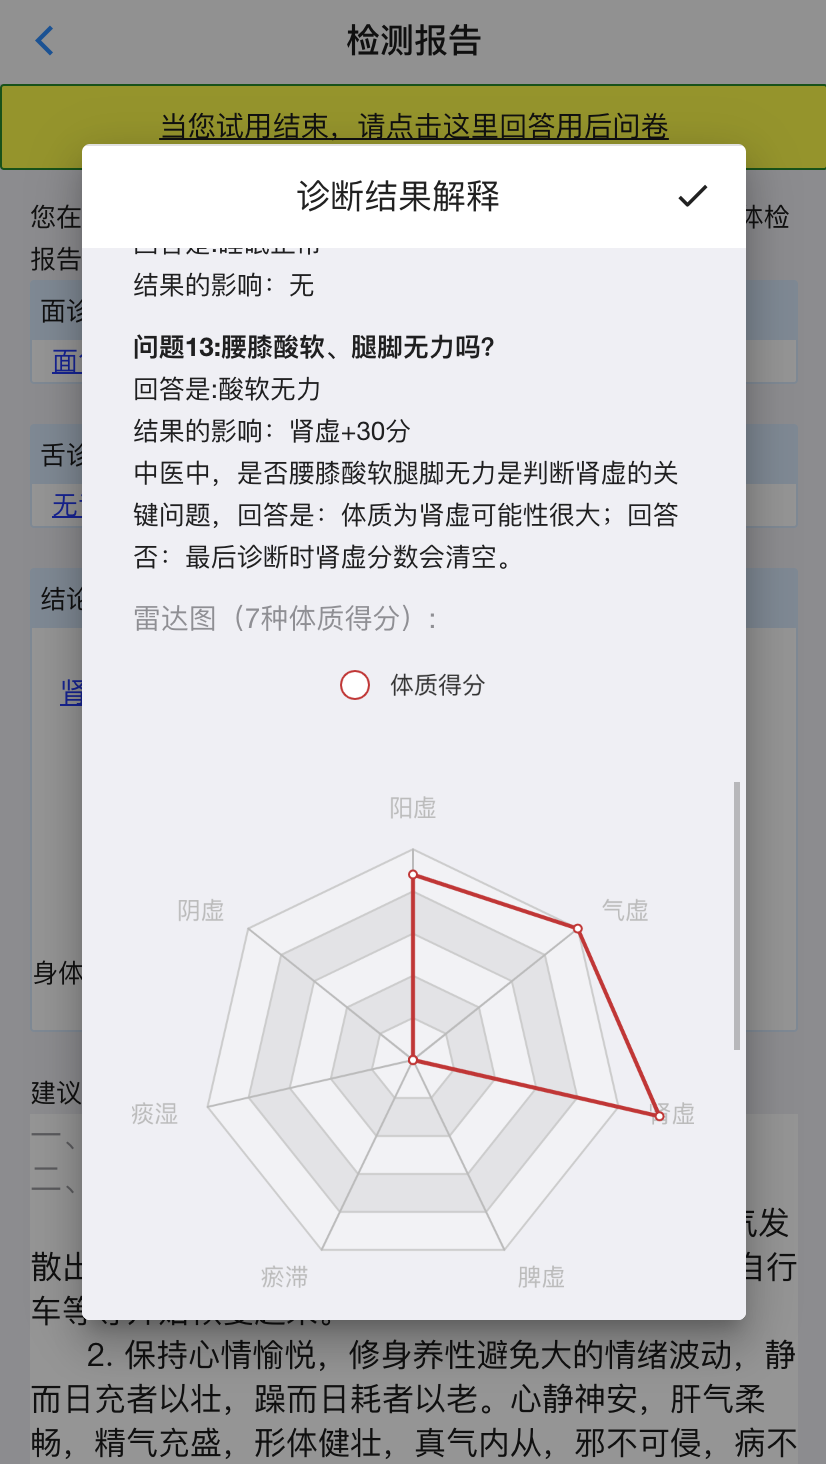
\includegraphics[width=4.5cm]{images/report8.png}
    }
    \subfigure[计算公式]{
        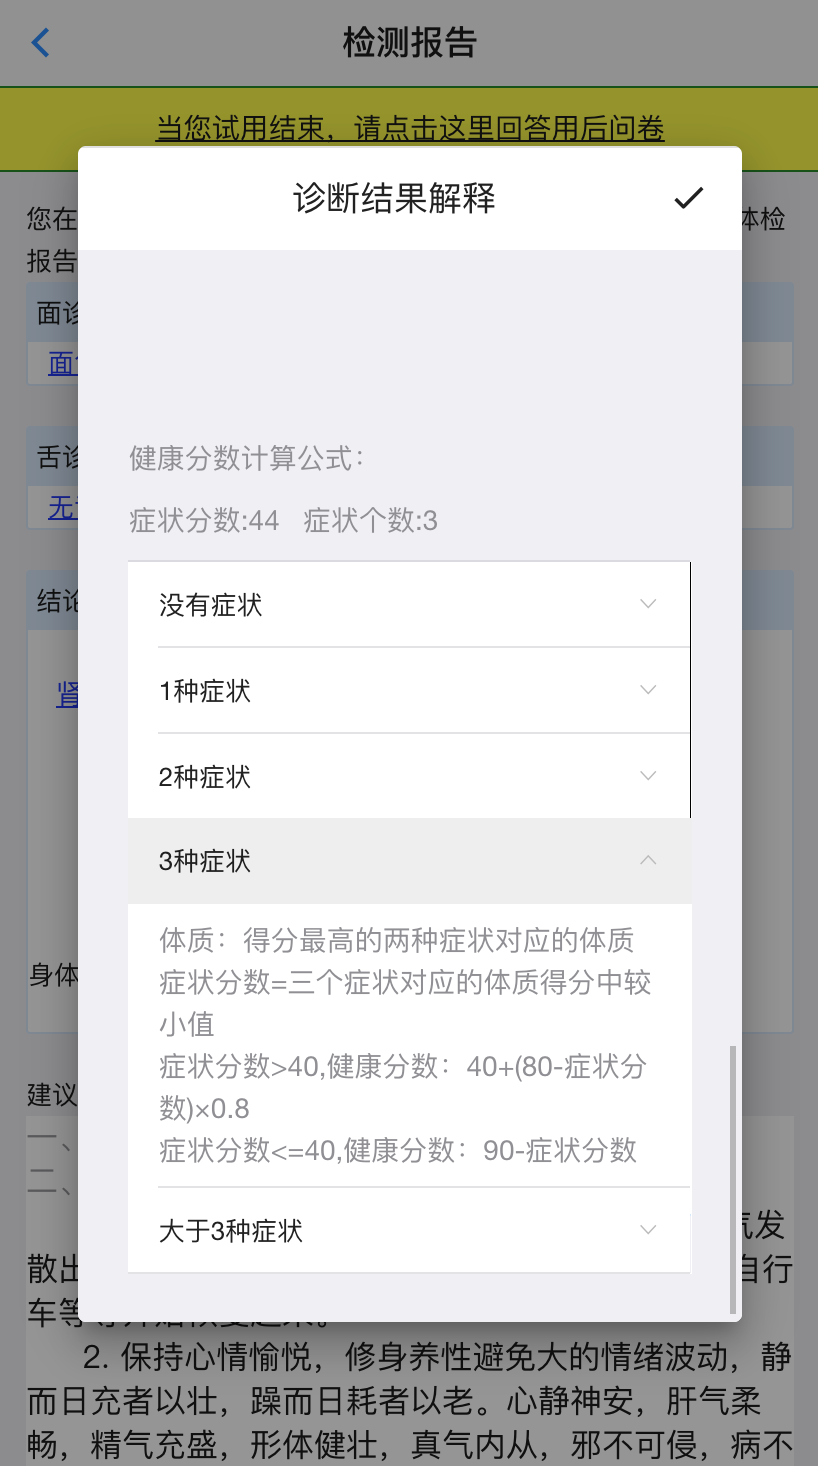
\includegraphics[width=4.5cm]{images/report9.png}
    }
    \caption{健康分数的解释}
    \label{fig:report_expalin_score}
\end{figure}

如图\ref{fig:report_expalin_score}所示,用户点击诊断页面的分数之后,弹窗里会显示分数相关的问题、雷达图和分数计算公式。

分数相关问题,展示了面诊舌诊对体质分数的影响和问诊对体质分数的影响,无影响的问题则不会显示。

用户每次回答一个问诊的问题,或者进行面诊舌诊断,都会对体质的倾向分数产生一定的影响。在规则系统中,体质倾向分数的变化分两种,一个是分数的累加,另一种是体质倾向分数的清空。

雷达图对体质分数进行了汇总,给用户展示最终个人的体质倾向的结果。

根据规则系统,解释页面的计算公式一共有5种类别。用户具体属于哪个类别,使用哪一套计算公式,是由用户当前的症状的个数来决定的。

我们使用选项卡的方式,将所有的打分计算公式全部暴露给用户,并且默认打开当前计算公式的选项卡。

\subsubsection{体质的解释}

\begin{figure}[htbp]
    \centering
    \subfigure[概念的解释]{
        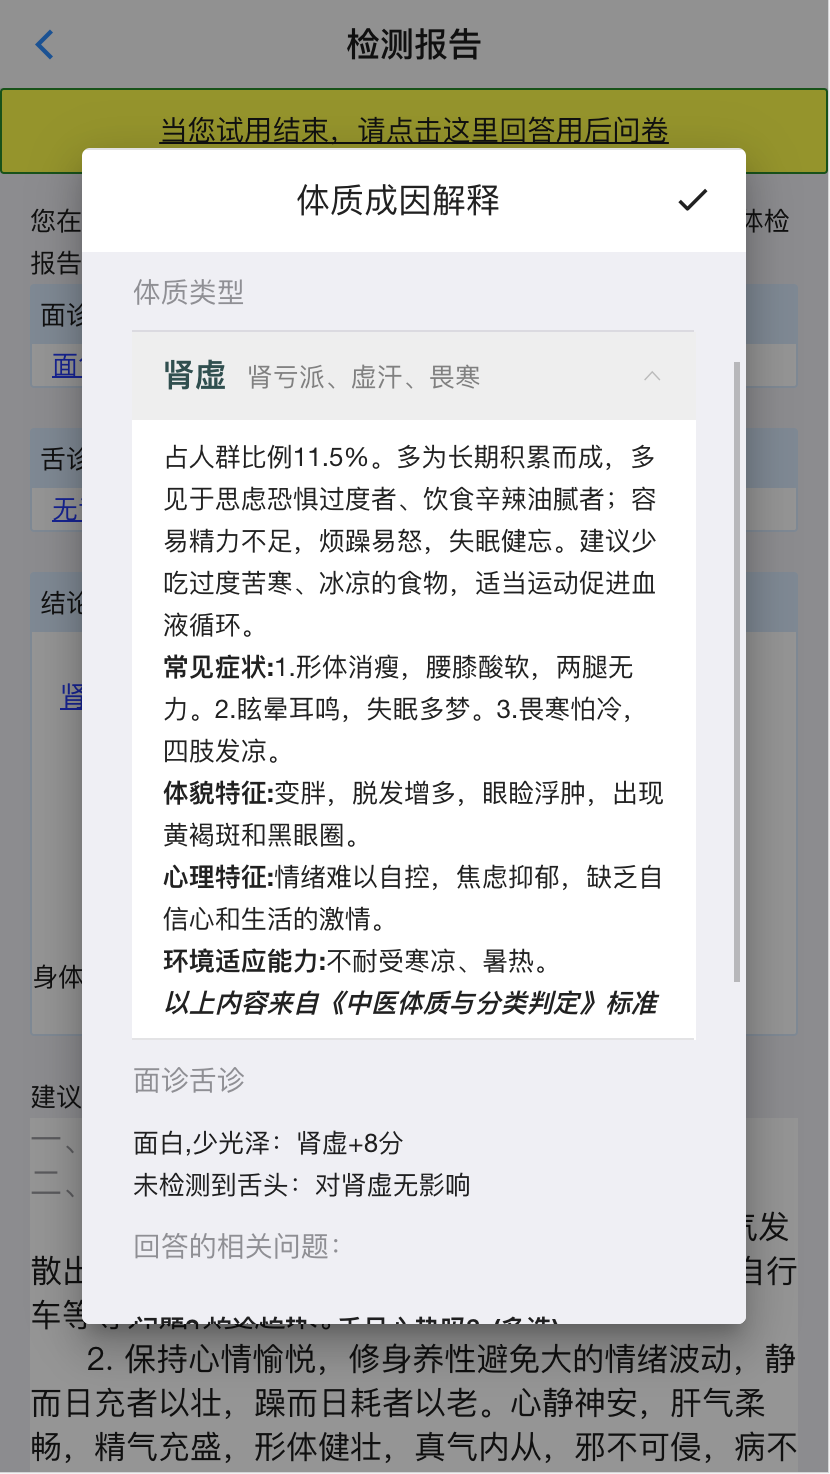
\includegraphics[width=4.5cm]{images/report5.png}
    }
    \subfigure[影响结果相关问题]{
        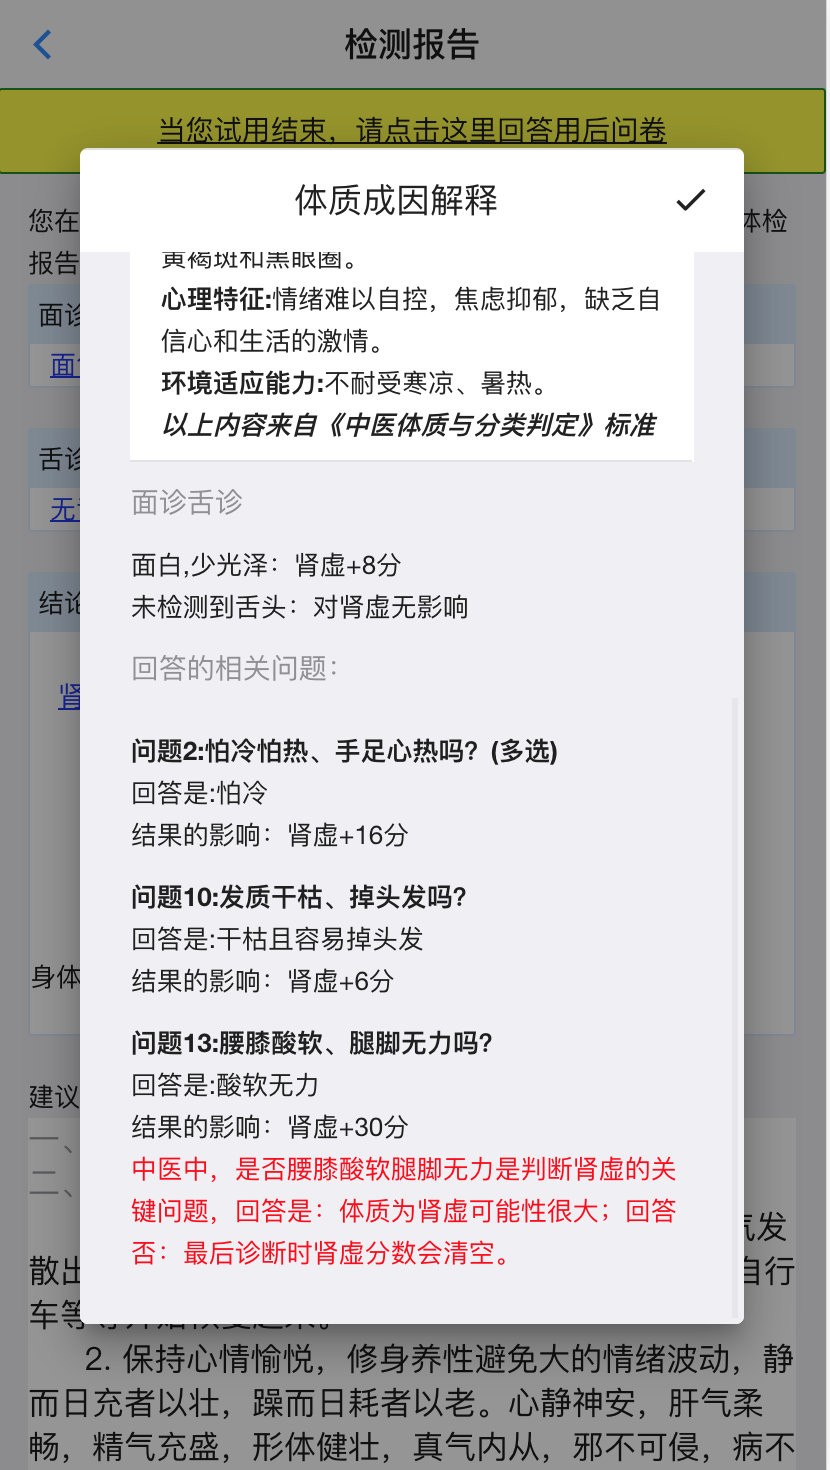
\includegraphics[width=4.5cm]{images/report6.png}
    }
    \caption{体质的解释}
    \label{fig:report_explain_phy_1}
\end{figure}

如图 \ref{fig:report_explain_phy_1} 所示:

(a) 在解释体质结果之前,我们首先对该体质的特征进行了说明,对体质的概念进行了解释。

(b) 后续,我们将规则系统判断时用到的相关的问题暴露给了用户。用户可以看到自己舌诊、面诊或者问诊中回答的某一个问题,对于该结果的影响。
% \section{反馈调研}
% 在新系统完成之后,我们采访了16名用户。
% 在本次调研过程中,用户试用的是同时有新旧界面的版本,除了第一次介绍使用的时候,我们会让用户两个版本都是使用一下,后续不做限时。用户具体使用的时候可以根据自己的喜好选择。
% 经过回访,新设计的界面达到了预期,大部分用户觉得使用起来更加地方便。
% 不过值得注意的是,也有少部分的用户喜欢原设计的将面诊,舌诊,问诊分开为三步进行的方式,因为这样比较符合日常生活的习惯。


\subsection{实验设计}

为了研究如何对面诊系统进行解释,我们设计了一个交互实现,通过线上实验结合深度访谈的形式进行。

\subsubsection{线上实验}
通过在各大社交平台发布海报,以及使用问卷星的样本服务招募志愿者, 经过筛选之后,我们一共招募了60位左右的用户。

每个用户的实验流程如下:

(1)用户通过扫描二维码,或者通过我们给定的链接,进入问卷星的调查问卷。

(2) 完成调查问卷之后,跳转到原型系统。通过调用问卷星提供的企业用户接口, 同时把问卷星的问卷id通过ssojump传给云中医在线应用。
通过ssojump中的问卷id, 完成自动登陆, 登陆的用户id为wjx-{问卷星id}。

(3) 在用户完成一次面诊之后,会在健康诊断页面下,看到一个跳转链接,可以选择填写用后问卷。

在实验过程中,用户会被随机分配到有解释的原型系统和无解释的原型系统。

\subsubsection{深度访谈}

定量的数据分析,我们无法得出哪些因变量如对结果的信任与是否有解释的相关性。为了继续研究解释的影响,同时理解为什么实验数据会呈现上述的特点,我们补充了一次深度访谈。

本次实验,我们同样实现了一个原型系统,界面和流程与上一个实验完全相同,但是去掉了用户登录时的随机分配用户角色,而是添加了一个开关。
当开关关闭的时候,系统不会对结果进行解释;当开关打开的时候,系统会对诊断过程和诊断结果进行详细的解释。

在使用过程中,我们首先让用户试用有解释或者没有解释的版本,鼓励用户在使用过程中随时自己内心的想法。然后我们切换开关,让用户再一次使用。最后对用户进行一次深度访谈。

\subsection{实验数据}
每个用户在参与实验之后,我们可以得到调查问卷的数据,云中医的使用日志,已经用后问卷的数据。

\subsubsection{可用数据}
本次实验可分析的数据来自调查问卷,用后问卷和实验平台的日志三个数据表,对应的可用数据如下:

调查问卷:序号,提交答卷时间,所用时间,来源,来源详情,IP,个人信息,我相信中医养生,了解中医养生,平时注重养生,经常去看中医,希望自己的生活方式更健康,对学习相关中医养生知识感兴趣,认为中医面诊可以了解健康情况,认为中医舌诊可以了解健康情况,认为智能系统可以自动评估健康情况,随机顺序的中医知识问题。
其中个人信息包括性别,年龄段,受教育水平,职业,城市,健康状态等。

用后问卷:序号,提交答卷时间,所用时间,来源,来源详情,IP,云中医的诊断结果,结果的信任程度,对结果的理解程度,是否愿意使用类似应用,随机顺序的中医知识问题。

用户使用日志: 序号,用户名,设备信息,操作名,操作信息,日期 。

\subsubsection{信息提取}
对于同一个用户在一次实验过程中,若调查问卷的ssojump参数为ID, 则此次用户操作记录的用户名为wjx-ID, 用户问卷的来源详情为wjx-ID。 
通过这个对应关系,我们就可以利用实验平台提供的问卷关联的功能,把三个表的信息,合并到一个表中,实验平台通过表格插件导出下载,最终得到特征如表\ref{tab:exp_data}所示。


\begin{table}[h]
    \centering
    \begin{tabular}{ll}
        \toprule
        字段 & 描述 \\ 
        \midrule
        序号 & 调查问卷序号 \\
        性别 & 男/女/未知 \\
        教育程度 & 本科以下/本科/本科以上 \\
        工作类型 & 计算机相关/计算机不相关 \\
        用户类型 & 解释/不解释 \\
        健康得分 & 云中医应用给出的分数 0-100 \\
        信任 & 对结果的信任程度 1-5 \\
        理解 & 对结果的理解程度 1-5 \\
        前健康知识得分 & 使用云中医之前的健康知识得分 \\
        后健康知识得分 & 使用云中医之后的健康知识得分 \\
        查看了哪些解释 & 使用过程中查看的解释类型 \\
        \bottomrule
    \end{tabular}
    \caption{实验数据汇总}
    \label{tab:exp_data}
\end{table}

经过处理之后,我们最终得到的数据图表 \ref{tab:exp_data}所示,对应的字段说明如下:

\begin{itemize}
  \item 工作类型: 根据调查问卷的数据,用户自由填写的职业类型有很多,为了便于分析,我们把 IT经理,IT软件设计, hr, it, 互联网, 技术研发, 技术研发人员, 技术经理, 电脑工程师, 研发, 科研, 程序员, 计算机, 软件工程师, 软件开发工程师, 通信, 通讯等归为it相关。

  \item  信任、理解: 这两个字段来自用后问卷调查表,取值范围为1-5的整数。

  \item  健康知识得分: 使用云中医应用前后的健康知识得分,使用的是用户回答正确中医知识的个数。

  \item  用户类型:用户使用的版本,包括原始版本或者添加了解释的版本。

  \item  查看了哪些解释: 通过检索日志中关键字获取,包括面诊过程,舌诊过程,体质术语介绍,诊断报告的:面诊结果,舌诊结果,健康分数,体质,分数计算公式等。
\end{itemize}

\subsection{实验结果}

\subsubsection{影响权重的解释方式}
在面诊舌诊和问诊中,都会涉及到本项的诊断对最终体质影响的权重。我们通过实验发现相对于柱状图的方式,雷达图更加适合该场景。

在权重解释这部分,用户不仅可以看到自己目前的舌相或者面相对应的特征,还能看到对每个体质影响的权重,该原型将最后诊断的规则系统部分规则暴露给了用户。
向用户解释这个权重的时候,我们使用了图表的方式向用户解释权重。如图 \ref{fig:question_weight} 所示,实验迭代的过程中我们先后实现了使用柱状图和雷达图的方式来展示权重。

\begin{figure}[htbp]
    \centering
    \subfigure[柱状图方式]{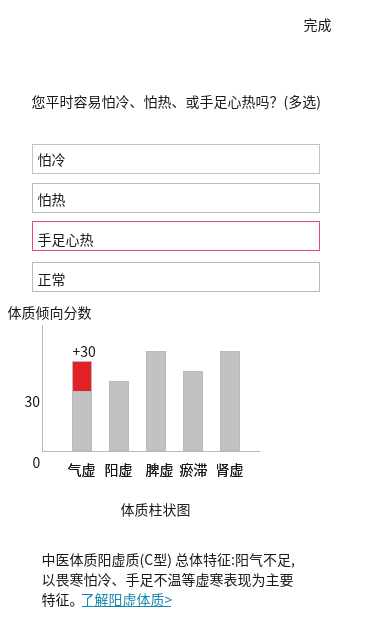
\includegraphics[height=10cm]{images/old3.png}}
    \subfigure[雷达图方式]{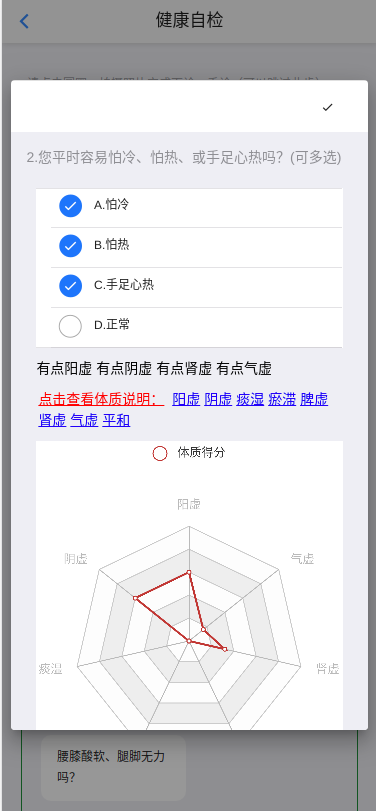
\includegraphics[height=10cm]{images/questions2.png}}
    \caption{影响权重的解释}
    \label{fig:question_weight}
\end{figure}

如图\ref{fig:question_weight}(a)所示,我们在设计中采用柱状图的方式向用户解释该问题对体质倾向影响的权重,其中通过红色突出显示本次出现变化的部分。
但是在实验过程中,经过用户反馈,我们发现在和用户自己健康相关的场景下,柱状图不适合用来解释影响权重。柱状图在权重差距较大的情况下可能会有一部分\myfont{突出}的比较高,有一个明显的缺点就是柱状图容易引起用户对自己身体情况的焦虑感。部分用户的反馈如下:
\myfont{然后他那个柱状图是太让人心慌了,那么片面的每道题给你一个那么高的值。}、
\myfont{下面那个柱状图非常吓人的,弹出来很高,让我有一种我的脾脏已经不行了的感觉。}

为了避免在解释影响权重过程中引起用户不必要的恐慌,我们需要一种相对"温和"的方式对影响权重进行解释,于是最终选用了雷达图的方式来解释影响权重。
如图\ref{fig:question_weight}(b)所示,雷达图从外观上来看会让数值的峰值不那么明显。

\subsubsection{日志分析结果}

通过对在线实验数据变量间的相关性分析,结果并没有体现出各个变量和是否看了解释的有强相关性,当前的解释方式对用户吸引力还不够。

根据日志数据,发现本次实验数据中,大多数参与者的完成质量非常差,具体有以下几个特点:

\begin{enumerate}
    \item 虽然我们在线上收集数据的时候,过滤了完成实验用时较短的样本,但是整体的完成实验的时间也是偏短,说明用户在填写问卷的时候没有认真思考。

    \item 日志数据中用户点击了解释的比例不到1/3,点了解释的用户中大部分也只点了面诊、舌诊、体质解释、结果解释中的一种,剩下的大部分用户并没有去点击去查看解释。
\end{enumerate}

% 同时实验分析,我们可以得出,增加解释可以提高用户对应中医知识的理解。

% 和看解释有关, 用 二元逻辑回归

% 把用户进行筛选,看了解释和没有看解释的

% 有解释的,看了没没看的(为什么看了,为什么没看), 

% 相关性分析,用于分析自变量

% 挑选相关性比较低的,放到后续的模型中 , 不加*,是很弱的 0.4-0.6比较强

% 了解中医养生,平时注重养生,了解中医养生
% 相信中医,了解中医

% 有没有看解释和it相关性不高

% 看了解释的影响:
% 独立样本t检验,差异性分析,没有显著差异

% 找最相似的不看解释的用户和看了解释的用户对比: 
% 对结果的信任和理解程度,两个样本没有显著差异



% 量化结果
\subsubsection{深度访谈结果}



通过深度访谈,我们发现日常面诊环境下,几乎所有的用户都更喜欢添加了解释的版本:\myfont{因为第一个版本其实和第二个版本得出来的诊断结果是一样的,它并不会说给我分数提高让我感觉更健康了,它只是说让我看清楚到底是什么问题,我觉得对我来说我是更喜欢第二个版本。}、
\myfont{喜欢有解释的,因为它有详细的解释啊。因为可以直接看到你的问题所在,就是可以解释这个症状对应什么问题。}

在验证了设计思路有效性的同时,我们也发现了添加可解释性的影响有以下结论:

\subsubsection{1.忽略解释的原因}
(1) 文字提示的形式不明显,不知道可以点击。

参与者被问到为什么没有点开解释查看时,他们的回答是:\myfont{直接看到图形界面了,没有注意到有文字解释。},\myfont{感觉文字不像是可以点的}、\myfont{对,不是很明显,我没注意}、\myfont{好像不太明显,因为我一开始以为是一个什么东西,注意力都在面诊}。
有参与者建议可以做成消息提醒的小红点的形式,利用用户的“强迫症”心理,吸引用户打开解释。

(2) 看到解释的提示,但是自己对结果没有疑惑。

两位参与者明确表示自己看到了解释,但是就是没有点,其中一位说道:\myfont{我觉得并不是说你所有的有显示可以点,我就一定要点},而另一位参与者则表示:\myfont{你像面白无光泽,就很直白的这个意思,我就能理解,为什么还要点进去看无光泽是什么意思?}


(3) 想尽快完成本地诊断的流程。
 另外一个让用户忽略实验原型中解释的原因是因为本次实验设置的实验流程过于繁琐,部分用户想尽快结束实验的流程,其中一位参与者解释说:\myfont{因为我想快点结束。};
 而另一位参与者也看到了解释,但是并没有选择点开:\myfont{我不会想去打开,因为我想要做下一题。}

\subsubsection{2.提高用户对诊断结果的接受程度}

(1) 用户知道背后的原理之后,如果结果不符合自己的预期,会尝试从自己方面的原因解释为什么不是这个结果。

当采访者知道自己的个人判断和系统给出的不一致时,他的反应是对于自己的判断产生怀疑而不是质疑系统给出的结果:\myfont{问题在我们吧,我也不知道。} 而其他的参与者在之后其背后原理之后,也表示对系统的错误可以接受:
\myfont{但你如果你说列出来三个可能的结果,你说你都有这三种结果都有可能。 我觉得这种我是可以去接受,里面如果有某一个和我的匹配就行了}、
\myfont{深度学习模型尽管它可能它训练的效果可能没有很完善,但是你加了模型进去以后,它确实是能反映出来个人健康一定的问题。}


(2) 提高对错误结果的接受程度。

在参与者知道深度学习需要大量的数据后,即使当前结果不太符合预期,也能理解目前数据量可能不足,有一定的错误率是正常的:
\myfont{也不能说完全不能接受,就像你前面也说了, 他说根据大数据样本去得出来的, 而且但这个可能并不符合每个人的情况很正常。}、
\myfont{等训练数据足够大了也许效果就会好很多。}

\subsubsection{3.增加对系统的信赖程度}

参访者认为系统用到了实际的深度学习的技术, 觉得更加可信赖:\myfont{但是你加了一个是深度学习模型进去,不管怎么样,它至少用到了一定的科学技术。}
另一位采访者觉得因为研发的机构比较权威,系统比较可靠:\myfont{我信当然信,你不觉得人们很容易有这种名牌效应,觉得牌子在这放着就不错。},而另一个参与者在知道本系统用到了中医药大学提供的诊断规则之后也表示:\myfont{我觉得你们比较权威。}

\subsubsection{4.对于提高中医的理解的帮助}
和我们预想的想法,虽然在第一次线上实验的时候,我们发现用户在使用系统之后的中医知识得分相较于使用系统之前的中医知识得分有稍微提高,但是经过访谈我们得到的结果是:
本文所使用的添加解释的方法,对于提高中医的理解帮助不大。

经过总结之后,用户反馈为解释文字太多,很难有学习兴趣:\myfont{因为像这种它给我诊断结果,包括它跟我说了什么东西,我只是一扫而过,我不会去刻意向去学习这个东西,因为只有我需要的话,我是做这一行的,或者说我对这很感兴趣,我肯定会去了解的,但我其实对中医什么的并不是多感兴趣,我只是大致看一下到底是什么东西,但我不会刻意去记去学这些东西。}、
\myfont{我觉得中医,但这种方式就是全是文字,我看的就是而且比较宽泛的文字,我看着就感觉没太有兴趣}、
\myfont{我觉得文字有点太多了,太密集了,找不到重点。}


\subsubsection{5.需要更合适的解释方法}
(1) 解释的形式。

除了通过文字的方式,参与者建议通过讲故事的形式,图文并茂,配上视频提高用户的学习兴趣:
\myfont{如果比较有兴趣的,像之前看过有一个老师做说那种形式,它可能做成一种游戏的形式,或者一种或者是一种讲故事的形式,它是有图画有文字的,会让你感觉更生动形象更加有趣。 }

(2) 解释的内容。

内容太多,太复杂,参与者建议只需要解释关键部分,判决依据就可以了:
\myfont{它写的有点复杂,感觉内容有点多啊}、
\myfont{但是我觉得他有点过于多了,比如问诊那里,感觉每一个下面不需要解释这么多。最终结果理解是充分解释就OK了。}



\section{本章小结}

本章分别介绍了客户端的实现以及利用实验平台进行的两个交互实验。两个实验分别介绍了原型系统的实现,实验的设计,最后介绍了实验的结果。
通过分析实验结果,我们发现本文提出的增加系统可用性的设计能够提高用户的交互体验;在可解释原型的实验过程中,我们发现对和健康相关的权重进行解释是,柱状图会引起用户的反感和恐慌,而雷达图能够避免出现这一情况。总的来说,增加系统的可解释性,对系统中的概念和结果进行解释,能够提高用户对结果的理解程度和对系统的信赖程度。



% 6.总结
\chapter{总结与展望}
\section{总结}
随着移动设备硬件水平的提高,各种日常场景下的健康应用随之出现;而在健康诊断信息化方面,人工智能的发展让许多健康诊断技术也能应用在实际生活中,其中就包括基于面部信息的健康诊断技术。我们针对日常场景下的面诊交互这一场景,发现虽然目前已有大量的日常健康的交互技术和大量的面诊信息化方法,但是主要都是针对专业人士或者在医疗诊所环境下使用,缺乏如何将面诊技术应用到日常场景下的研究。本文按照发现问题、寻求解决方案、确定解决方案、系统实现、设计实现并验证的步骤,做了以下的工作:

\begin{enumerate}
	\item 使用云中医作为技术探针,设计了定性实验,通过社交平台发布海报募了参与者参与实验并对在实验过程中及结束后对参与者进行了深度访谈以获取实验数据。
	
	\item 结合实验数据,分析出日常场景下面诊技术潜在的使用场景包括了解身体状态和医患沟通的工具,同时发现面诊技术在日常场景下存在着自适应性、实用性和敏感性的问题,特别的是作为健康诊断工具的时候,可能会影响用户的情绪和对系统的信赖程度。针对这些可能存在的问题,本文同时提出了对应:增加可变性、系统透明性、日常可用性的设计方案。

	\item 为了方便交互实验,设计并实现了支持面诊交互实验的实验平台,跨平台的实验屏蔽了用户不同设备类型可能会遇到的问题,统一的模型管理提高了模型的稳定性,方便新模型的接入和替换;任务管理对一次诊断任务进行了分解,提高多用户请求时的并发度;用户操作记录管理和问卷关联的功能,能够更加方便地设计新的问卷和采集用户信息,对用户细粒度的行为进行分析成为可能。
	
	\item 基于定性研究的设计方案,我们在实验平台上进行,在设计方案的迭代过程中,探索了如何实现可用性的设计、如何对结果影响的权重进行展示、如何对系统进行解释等,最终分别实现了基于可用性和透明性的设计方案的应用原型。

	\item 对本文提出的可用性设计和透明性设计在实验平台上进行了实验,验证了实验平台功能的同时探索了对应的设计方案的效果。
\end{enumerate}


% 不足之处


% 展望
\section{展望}
由于时间和精力有限,本文在后续的实验阶段,只通过实验平台对交互问题中的可用性和透明性的问题进行了验证和探索。未来可进行的交互研究工作如下:

\begin{enumerate}
	\item 设计如何增加系统的自适应。系统的自适应性包括对用户的自适应和对上下文的自适应。用户自适应性设计的实现需要采集用户信息,并分析出用户信息中和个人健康的相关点,上下文则包括短期的天气节气上下文信息和长期的用户使用记录。如何实现系统对用户数据的自适应性,并且如何在养生建议等步骤中加入上下文信息,还需要进一步地探索和设计实验。

	\item 与用户的日常行为融合。日常健康诊断在某些用户中不是一个日常的行为,用户不一定习惯于每天为专门为了检测自己的健康情况打开相机,而大多数用户会有自拍的习惯。面诊技术的特殊性在于它基于面部信息,如何将自拍和健康诊断结合起来,也是一个非常有意思的研究点。

	\item 探索日常诊断的社交功能。在第二章中,我们讨论了面诊信息的分享的特殊性:一方面有的用户考虑个人照片会泄露隐私,另一方面用户希望通过分享和其他人交流健康的知识。同时,在大量相关研究中,添加社交功能也是促进用户持续使用的常用方法之一。那么如何设计一个在不泄露用户隐私信息的情况下,实现用户之间的面部诊断信息分享和交流,还需要进一步地研究。
\end{enumerate}


% 同时,本文提出的实验平台是为了方便面诊交互实验而设计,因此在用户系统的基础上,添加深度访谈数据管理的功能也是非常必要的。

\backmatter
% 后置部分包含参考文献、声明页(自动生成)等


\bibliography{bibliography}
% % 打印参考文献列表

% 致谢
\chapter{致谢}

% 总结这三年的经历


% 感谢导师
感谢丁向华老师一直以来的包容,和工作方面的支持。

% 感谢实验室其他老师
感谢实验室顾老师和卢老师

% 感谢实验室其他同学
感谢宋励师兄,刘鹏师兄,实验室其他同学。

% 感谢家人和公司的同事


\end{document}
